\documentclass[12pt]{article}
\usepackage{amsmath,amscd,amssymb,amsthm,enumerate,verbatim,palatino,parskip,graphicx}
\usepackage{tikz,titlesec}

\titleformat{\section}
  {\newpage\rmfamily\Large\bfseries}{}{0em}{Lecture \thesection:~}
\titlespacing*{\section}{0pt}{3.25ex plus 1ex minus .2ex}{1.5ex plus .2ex}

\usetikzlibrary{matrix,arrows,decorations.pathmorphing}
\usepackage{amsbsy,anysize,tikz-cd}
\marginsize{2.3cm}{2.3cm}{2cm}{2.4cm}

\renewcommand\vec[1]{\ensuremath\boldsymbol{#1}}
\usepackage[T1]{fontenc}
\usepackage{hyperref}

\usepackage{tikz}
\usetikzlibrary{arrows,decorations.markings}

% Structure of irreps of sl(2,C)

\newcommand{\sltwo}{\begin{center}
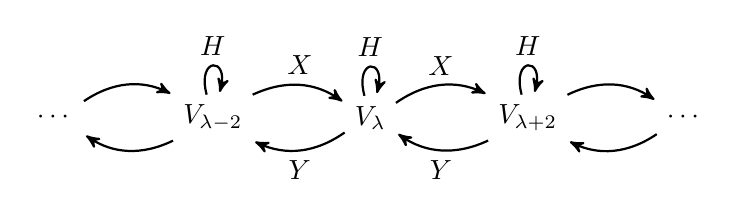
\begin{tikzpicture}[->,>=stealth',shorten >=1pt,auto,node distance=2cm,
  thick]

  \node (1) {$V_{\lambda}$};
  \node (2) [right of=1] {$V_{\lambda+2}$};
  \node (3) [left of=1] {$V_{\lambda-2}$};
  \node (4) [left of=3] {$\cdots$};
  \node (5) [right of=2] {$\cdots$};

  \path
    (1) edge [bend left] node [above] {$X$} (2)
        edge [bend left] node [below] {$Y$} (3)
        edge [loop above] node {$H$} (1)
    (2) edge [bend left] node [below] {$Y$} (1)
        edge [bend left] (5)
        edge [loop above] node {$H$} (2)
    (3) edge [bend left] node [above] {$X$} (1)
        edge [loop above] node {$H$} (3)
        edge [bend left] (4)
    (4) edge [bend left] (3)
    (5) edge [bend left] (2);
\end{tikzpicture}\end{center}}

% The roots of sl(3,C)

\newcommand{\slthree}{\begin{center}
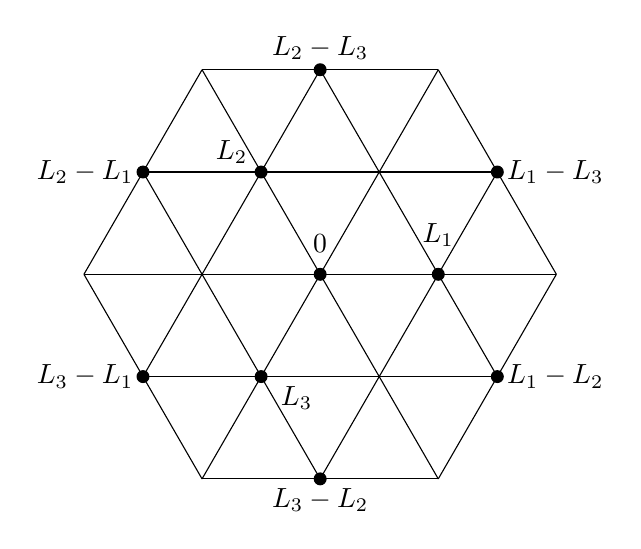
\begin{tikzpicture}[scale=1.5]
  \draw (240:2) -- (60:2);
  \draw (120:2) -- (300:2);
  \draw (60:2) -- (0:2);
  \draw (240:2) -- (180:2);
  \draw (180:2) -- (120:2);
  \draw (0:2) -- (300:2);
  \draw (120:2) -- (60:2);
  \draw (240:2) -- (300:2);
  \draw (180:2) -- (0:2);
  \draw (210:{2*sin{60}}) -- (330:{2*sin{60}});
  \draw (150:{2*sin{60}}) -- (30:{2*sin{60}});
  \draw (150:{2*sin{60}}) -- (270:{2*sin{60}});
  \draw (90:{2*sin{60}}) -- (330:{2*sin{60}});
  \draw (90:{2*sin{60}}) -- (210:{2*sin{60}});
  \draw (30:{2*sin{60}}) -- (270:{2*sin{60}});
  \draw[fill] (30:{2*sin{60}}) circle [radius=0.05];
  \draw[fill] (90:{2*sin{60}}) circle [radius=0.05];
  \draw[fill] (150:{2*sin{60}}) circle [radius=0.05];
  \draw[fill] (210:{2*sin{60}}) circle [radius=0.05];
  \draw[fill] (270:{2*sin{60}}) circle [radius=0.05];
  \draw[fill] (330:{2*sin{60}}) circle [radius=0.05];
  \draw[fill] (0,0) circle [radius=0.05];
  \draw[fill] (0:1) circle [radius=0.05];
  \draw[fill] (120:1) circle [radius=0.05];
  \draw[fill] (240:1) circle [radius=0.05];
  \node [above] at (0,0.1) {$0$};
  \node [above] at (1,0.15) {$L_1$};
  \node [below] at ({cos{120}-0.25},sin{120}+0.35) {$L_2$};
  \node [below] at ({cos{240}+0.3},sin{240}) {$L_3$};
  \node (1) [right] at (30:{2*sin{60}}) {$L_1-L_3$};
  \node (2) [above] at (90:{2*sin{60}}) {$L_2-L_3$};
  \node (3) [left] at (150:{2*sin{60}}) {$L_2-L_1$};
  \node (4) [left] at (210:{2*sin{60}}) {$L_3-L_1$};
  \node (5) [below] at (270:{2*sin{60}}) {$L_3-L_2$};
  \node (6) [right] at (330:{2*sin{60}}) {$L_1-L_2$};
\end{tikzpicture}\end{center}}

% And now for a diagram illustrating the adjoint action of root spaces on one another.

\newcommand{\sladj}{\begin{center}
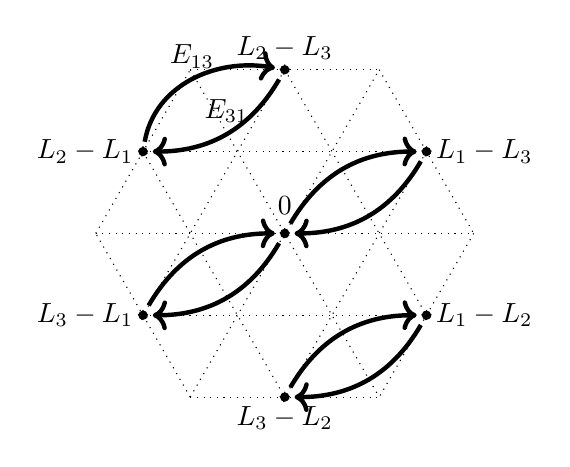
\begin{tikzpicture}[scale=1.2,dotted]
  \draw (240:2) -- (60:2);
  \draw (120:2) -- (300:2);
  \draw (60:2) -- (0:2);
  \draw (240:2) -- (180:2);
  \draw (180:2) -- (120:2);
  \draw (0:2) -- (300:2);
  \draw (120:2) -- (60:2);
  \draw (240:2) -- (300:2);
  \draw (180:2) -- (0:2);
  \draw (210:{2*sin{60}}) -- (330:{2*sin{60}});
  \draw (150:{2*sin{60}}) -- (30:{2*sin{60}});
  \draw (150:{2*sin{60}}) -- (270:{2*sin{60}});
  \draw (90:{2*sin{60}}) -- (330:{2*sin{60}});
  \draw (90:{2*sin{60}}) -- (210:{2*sin{60}});
  \draw (30:{2*sin{60}}) -- (270:{2*sin{60}});
  \draw[fill] (30:{2*sin{60}}) circle [radius=0.05];
  \draw[fill] (90:{2*sin{60}}) circle [radius=0.05];
  \draw[fill] (150:{2*sin{60}}) circle [radius=0.05];
  \draw[fill] (210:{2*sin{60}}) circle [radius=0.05];
  \draw[fill] (270:{2*sin{60}}) circle [radius=0.05];
  \draw[fill] (330:{2*sin{60}}) circle [radius=0.05];
  \draw[fill] (0,0) circle [radius=0.05];
  \node [above] at (0,0.1) {$0$};
  \node (0) at (0,0) {};
  \node [right] at (30:{2*sin{60}}) {$L_1-L_3$};
  \node (1) at (30:{2*sin{60}}) {};
  \node [above] at (90:{2*sin{60}}) {$L_2-L_3$};
  \node (2) at (90:{2*sin{60}}) {};
  \node [left] at (150:{2*sin{60}}) {$L_2-L_1$};
  \node (3) at (150:{2*sin{60}}) {};
  \node [left] at (210:{2*sin{60}}) {$L_3-L_1$};
  \node (4) at (210:{2*sin{60}}) {};
  \node [below] at (270:{2*sin{60}}) {$L_3-L_2$};
  \node (5) at (270:{2*sin{60}}) {};
  \node [right] at (330:{2*sin{60}}) {$L_1-L_2$};
  \node (6) at (330:{2*sin{60}}) {};
  \path[ultra thick,solid,->] 
  (3) edge [out=80,in=170] node [above] {$E_{13}$} (2)
  (2) edge [bend left] node [above] {$E_{31}$} (3)
  (4) edge [bend left] (0)
  (0) edge [bend left] (4)
  (0) edge [bend left] (1)
  (1) edge [bend left] (0)
  (5) edge [bend left] (6)
  (6) edge [bend left] (5);
\end{tikzpicture}
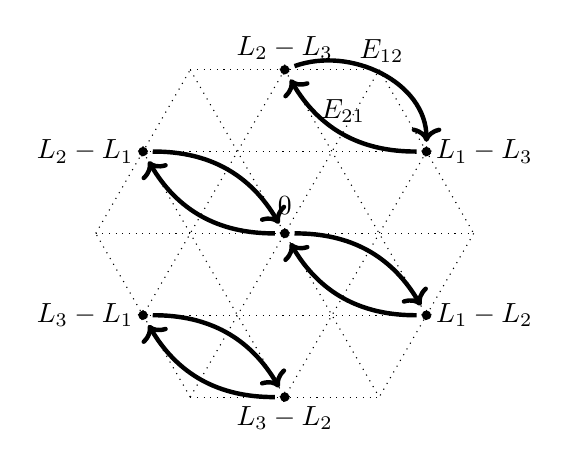
\begin{tikzpicture}[scale=1.2,dotted]
  \draw (240:2) -- (60:2);
  \draw (120:2) -- (300:2);
  \draw (60:2) -- (0:2);
  \draw (240:2) -- (180:2);
  \draw (180:2) -- (120:2);
  \draw (0:2) -- (300:2);
  \draw (120:2) -- (60:2);
  \draw (240:2) -- (300:2);
  \draw (180:2) -- (0:2);
  \draw (210:{2*sin{60}}) -- (330:{2*sin{60}});
  \draw (150:{2*sin{60}}) -- (30:{2*sin{60}});
  \draw (150:{2*sin{60}}) -- (270:{2*sin{60}});
  \draw (90:{2*sin{60}}) -- (330:{2*sin{60}});
  \draw (90:{2*sin{60}}) -- (210:{2*sin{60}});
  \draw (30:{2*sin{60}}) -- (270:{2*sin{60}});
  \draw[fill] (30:{2*sin{60}}) circle [radius=0.05];
  \draw[fill] (90:{2*sin{60}}) circle [radius=0.05];
  \draw[fill] (150:{2*sin{60}}) circle [radius=0.05];
  \draw[fill] (210:{2*sin{60}}) circle [radius=0.05];
  \draw[fill] (270:{2*sin{60}}) circle [radius=0.05];
  \draw[fill] (330:{2*sin{60}}) circle [radius=0.05];
  \draw[fill] (0,0) circle [radius=0.05];
  \node [above] at (0,0.1) {$0$};
  \node (0) at (0,0) {};
  \node [right] at (30:{2*sin{60}}) {$L_1-L_3$};
  \node (1) at (30:{2*sin{60}}) {};
  \node [above] at (90:{2*sin{60}}) {$L_2-L_3$};
  \node (2) at (90:{2*sin{60}}) {};
  \node [left] at (150:{2*sin{60}}) {$L_2-L_1$};
  \node (3) at (150:{2*sin{60}}) {};
  \node [left] at (210:{2*sin{60}}) {$L_3-L_1$};
  \node (4) at (210:{2*sin{60}}) {};
  \node [below] at (270:{2*sin{60}}) {$L_3-L_2$};
  \node (5) at (270:{2*sin{60}}) {};
  \node [right] at (330:{2*sin{60}}) {$L_1-L_2$};
  \node (6) at (330:{2*sin{60}}) {};
  \path[ultra thick,solid,->] 
  (2) edge [in=90,out=20] node [above] {$E_{12}$} (1)
  (1) edge [bend left] node [above] {$E_{21}$} (2)
  (3) edge [bend left] (0)
  (0) edge [bend left] (3)
  (0) edge [bend left] (6)
  (6) edge [bend left] (0)
  (4) edge [bend left] (5)
  (5) edge [bend left] (4);
\end{tikzpicture}
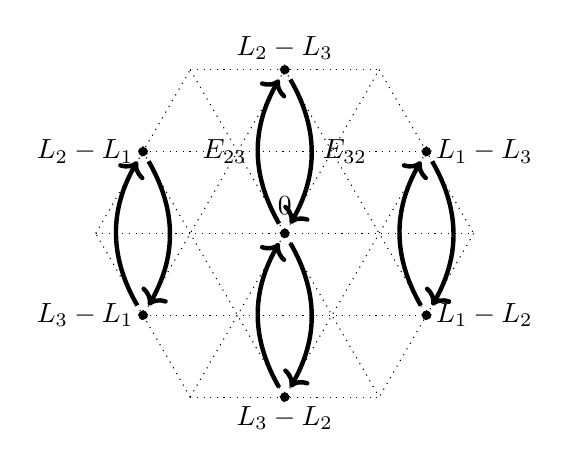
\begin{tikzpicture}[scale=1.2,dotted]
  \draw (240:2) -- (60:2);
  \draw (120:2) -- (300:2);
  \draw (60:2) -- (0:2);
  \draw (240:2) -- (180:2);
  \draw (180:2) -- (120:2);
  \draw (0:2) -- (300:2);
  \draw (120:2) -- (60:2);
  \draw (240:2) -- (300:2);
  \draw (180:2) -- (0:2);
  \draw (210:{2*sin{60}}) -- (330:{2*sin{60}});
  \draw (150:{2*sin{60}}) -- (30:{2*sin{60}});
  \draw (150:{2*sin{60}}) -- (270:{2*sin{60}});
  \draw (90:{2*sin{60}}) -- (330:{2*sin{60}});
  \draw (90:{2*sin{60}}) -- (210:{2*sin{60}});
  \draw (30:{2*sin{60}}) -- (270:{2*sin{60}});
  \draw[fill] (30:{2*sin{60}}) circle [radius=0.05];
  \draw[fill] (90:{2*sin{60}}) circle [radius=0.05];
  \draw[fill] (150:{2*sin{60}}) circle [radius=0.05];
  \draw[fill] (210:{2*sin{60}}) circle [radius=0.05];
  \draw[fill] (270:{2*sin{60}}) circle [radius=0.05];
  \draw[fill] (330:{2*sin{60}}) circle [radius=0.05];
  \draw[fill] (0,0) circle [radius=0.05];
  \node [above] at (0,0.1) {$0$};
  \node (0) at (0,0) {};
  \node [right] at (30:{2*sin{60}}) {$L_1-L_3$};
  \node (1) at (30:{2*sin{60}}) {};
  \node [above] at (90:{2*sin{60}}) {$L_2-L_3$};
  \node (2) at (90:{2*sin{60}}) {};
  \node [left] at (150:{2*sin{60}}) {$L_2-L_1$};
  \node (3) at (150:{2*sin{60}}) {};
  \node [left] at (210:{2*sin{60}}) {$L_3-L_1$};
  \node (4) at (210:{2*sin{60}}) {};
  \node [below] at (270:{2*sin{60}}) {$L_3-L_2$};
  \node (5) at (270:{2*sin{60}}) {};
  \node [right] at (330:{2*sin{60}}) {$L_1-L_2$};
  \node (6) at (330:{2*sin{60}}) {};
  \path[ultra thick,solid,->] 
  (0) edge [bend left] node [left] {$E_{23}$} (2)
  (2) edge [bend left] node [right] {$E_{32}$} (0)
  (0) edge [bend left] (5)
  (5) edge [bend left] (0)
  (1) edge [bend left] (6)
  (6) edge [bend left] (1)
  (4) edge [bend left] (3)
  (3) edge [bend left] (4);
\end{tikzpicture}\end{center}}

\newcommand{\slhwv}{\begin{center}
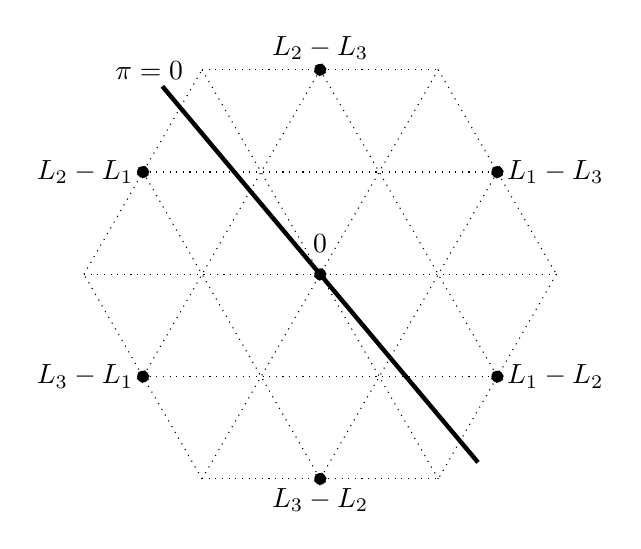
\begin{tikzpicture}[scale=1.5,dotted]
  \draw (240:2) -- (60:2);
  \draw (120:2) -- (300:2);
  \draw (60:2) -- (0:2);
  \draw (240:2) -- (180:2);
  \draw (180:2) -- (120:2);
  \draw (0:2) -- (300:2);
  \draw (120:2) -- (60:2);
  \draw (240:2) -- (300:2);
  \draw (180:2) -- (0:2);
  \draw (210:{2*sin{60}}) -- (330:{2*sin{60}});
  \draw (150:{2*sin{60}}) -- (30:{2*sin{60}});
  \draw (150:{2*sin{60}}) -- (270:{2*sin{60}});
  \draw (90:{2*sin{60}}) -- (330:{2*sin{60}});
  \draw (90:{2*sin{60}}) -- (210:{2*sin{60}});
  \draw (30:{2*sin{60}}) -- (270:{2*sin{60}});
  \draw[fill] (30:{2*sin{60}}) circle [radius=0.05];
  \draw[fill] (90:{2*sin{60}}) circle [radius=0.05];
  \draw[fill] (150:{2*sin{60}}) circle [radius=0.05];
  \draw[fill] (210:{2*sin{60}}) circle [radius=0.05];
  \draw[fill] (270:{2*sin{60}}) circle [radius=0.05];
  \draw[fill] (330:{2*sin{60}}) circle [radius=0.05];
  \draw[fill] (0,0) circle [radius=0.05];
  \node [above] at (0,0.1) {$0$};
  \node (0) at (0,0) {};
  \node [right] at (30:{2*sin{60}}) {$L_1-L_3$};
  \node (1) at (30:{2*sin{60}}) {};
  \node [above] at (90:{2*sin{60}}) {$L_2-L_3$};
  \node (2) at (90:{2*sin{60}}) {};
  \node [left] at (150:{2*sin{60}}) {$L_2-L_1$};
  \node (3) at (150:{2*sin{60}}) {};
  \node [left] at (210:{2*sin{60}}) {$L_3-L_1$};
  \node (4) at (210:{2*sin{60}}) {};
  \node [below] at (270:{2*sin{60}}) {$L_3-L_2$};
  \node (5) at (270:{2*sin{60}}) {};
  \node [right] at (330:{2*sin{60}}) {$L_1-L_2$};
  \node (6) at (330:{2*sin{60}}) {};
  \draw[ultra thick,solid] (310:{2.4*sin{60}}) -- (130:{2.4*sin{60}});
  \node at (130:{2.6*sin{60}}) {$\pi=0$};
\end{tikzpicture}\end{center}}

\newcommand{\sltritant}{\begin{center}
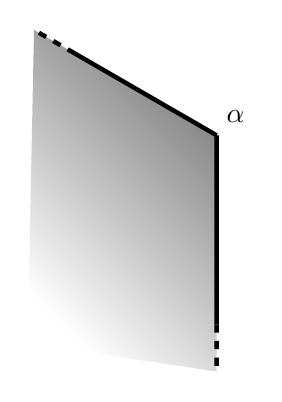
\begin{tikzpicture}[scale=1.2]
  \node at (0.2,0.2) {$\alpha$};
  \shade [shading angle=-45]
      (0,-2.5) -- (0,0) -- (150:2.23205080757) -- (-2,-2.2) -- cycle;
  \draw [ultra thick]
     (0,0) -- (0,-2)
     (0,0) -- (150:1.73205080757);
  \draw [ultra thick,dashed]
     (0,-2) -- (0,-2.5)
     (150:1.73205080757) -- (150:2.23205080757);
\end{tikzpicture}
\end{center}}

% The weight diagram for the standard representation of SU(3)

\newcommand{\slthreestd}{\begin{center}
\begin{tikzpicture}[scale=2,dotted]
  \draw (-1,0) -- (1,0);
  \draw (120:1) -- (60:1);
  \draw (240:1) -- (300:1);
  \draw (240:1) -- (60:1);
  \draw (120:1) -- (300:1);
  \draw (120:1) -- (180:1);
  \draw (180:1) -- (240:1);
  \draw (300:1) -- (1,0);
  \draw (1,0) -- (60:1);
  \draw[fill] (120:1) circle [radius=0.05];
  \draw[fill] (240:1) circle [radius=0.05];
  \draw[fill] (1,0) circle [radius=0.05];
  \node [above] at (0,0.1) {$0$};
  \node [above] at (1,0.15) {$L_1$};
  \node [below] at ({cos{120}-0.25},sin{120}+0.35) {$L_2$};
  \node [below] at ({cos{240}+0.3},sin{240}) {$L_3$};
\end{tikzpicture}\end{center}}

\newcommand{\slthreedual}{\begin{center}
\begin{tikzpicture}[scale=2,dotted]
  \draw (-1,0) -- (1,0);
  \draw (120:1) -- (60:1);
  \draw (240:1) -- (300:1);
  \draw (240:1) -- (60:1);
  \draw (120:1) -- (300:1);
  \draw (120:1) -- (180:1);
  \draw (180:1) -- (240:1);
  \draw (300:1) -- (1,0);
  \draw (1,0) -- (60:1);
  \draw[fill] (60:1) circle [radius=0.05];
  \draw[fill] (300:1) circle [radius=0.05];
  \draw[fill] (-1,0) circle [radius=0.05];
  \node [above] at (0,0.1) {$0$};
  \node at (-1.3,0) {$-L_1$};
  \node [below] at ({cos{60}+0.25},sin{60}+0.35) {$-L_2$};
  \node [below] at ({cos{300}+0.3},sin{300}) {$-L_3$};
\end{tikzpicture}\end{center}}

% The root diagram again, without L_1, L_2, L_3

\newcommand{\sladjwt}{\begin{center}
\begin{tikzpicture}[scale=1.5,dotted,bigger node/.style={fill=black,circle,draw,text=white,inner sep=1pt,font=\boldmath}]
  \draw (240:2) -- (60:2);
  \draw (120:2) -- (300:2);
  \draw (60:2) -- (0:2);
  \draw (240:2) -- (180:2);
  \draw (180:2) -- (120:2);
  \draw (0:2) -- (300:2);
  \draw (120:2) -- (60:2);
  \draw (240:2) -- (300:2);
  \draw (180:2) -- (0:2);
  \draw (210:{2*sin{60}}) -- (330:{2*sin{60}});
  \draw (150:{2*sin{60}}) -- (30:{2*sin{60}});
  \draw (150:{2*sin{60}}) -- (270:{2*sin{60}});
  \draw (90:{2*sin{60}}) -- (330:{2*sin{60}});
  \draw (90:{2*sin{60}}) -- (210:{2*sin{60}});
  \draw (30:{2*sin{60}}) -- (270:{2*sin{60}});
  \draw[fill] (30:{2*sin{60}}) circle [radius=0.05];
  \draw[fill] (90:{2*sin{60}}) circle [radius=0.05];
  \draw[fill] (150:{2*sin{60}}) circle [radius=0.05];
  \draw[fill] (210:{2*sin{60}}) circle [radius=0.05];
  \draw[fill] (270:{2*sin{60}}) circle [radius=0.05];
  \draw[fill] (330:{2*sin{60}}) circle [radius=0.05];
  \draw[fill] (0,0) circle [radius=0.05];
  \node [above] at (0,0.3) {$0$};
  \node[bigger node] (0) at (0,0) {2};
  \node [right] at (30:{2*sin{60}}) {$L_1-L_3$};
  \node (1) at (30:{2*sin{60}}) {};
  \node [above] at (90:{2*sin{60}}) {$L_2-L_3$};
  \node (2) at (90:{2*sin{60}}) {};
  \node [left] at (150:{2*sin{60}}) {$L_2-L_1$};
  \node (3) at (150:{2*sin{60}}) {};
  \node [left] at (210:{2*sin{60}}) {$L_3-L_1$};
  \node (4) at (210:{2*sin{60}}) {};
  \node [below] at (270:{2*sin{60}}) {$L_3-L_2$};
  \node (5) at (270:{2*sin{60}}) {};
  \node [right] at (330:{2*sin{60}}) {$L_1-L_2$};
  \node (6) at (330:{2*sin{60}}) {};
\end{tikzpicture}\end{center}}

% Weight diagram for the tensor square of the standard representation of SU(3)

\newcommand{\sltensq}[1]{\begin{center}
\begin{tikzpicture}[scale=#1*1.5,dotted,bigger node/.style={fill=black,circle,draw,text=white,inner sep=1pt,font=\boldmath}]
  \draw (-1,0) -- (2,0);
  \draw (120:2) -- (300:2);
  \draw (240:2) -- (60:2);
  \draw (120:2) -- (60:2);
  \draw (240:2) -- (300:2);
  \draw (60:2) -- (2,0);
  \draw (300:2) -- (2,0);
  \draw (0,{2*sin{60}}) -- (-1,0);
  \draw (0,{-2*sin{60}}) -- (-1,0);
  \draw (0,{2*sin{60}}) -- ({1+cos{60}},-{sin{60}});
  \draw (0,{-2*sin{60}}) -- ({1+cos{60}},{sin{60}});
  \draw (-1,{sin{60}}) -- ({1+cos{60}},{sin{60}});
  \draw (-1,{-sin{60}}) -- ({1+cos{60}},{-sin{60}});
  \draw[fill] (120:2) circle [radius=0.05];
  \draw[fill] (240:2) circle [radius=0.05];
  \draw[fill] (2,0) circle [radius=0.05];
  \node[bigger node] at (60:1) {2};
  \node[bigger node] at (300:1) {2};
  \node[bigger node] at (-1,0) {2};
  \node at (0,0) {$0$};
\end{tikzpicture}\end{center}}

\newcommand{\slsymsq}[1]{\begin{center}
\begin{tikzpicture}[scale=#1*1.5,dotted]
  \draw (-1,0) -- (2,0);
  \draw (120:2) -- (300:2);
  \draw (240:2) -- (60:2);
  \draw (120:2) -- (60:2);
  \draw (240:2) -- (300:2);
  \draw (60:2) -- (2,0);
  \draw (300:2) -- (2,0);
  \draw (0,{2*sin{60}}) -- (-1,0);
  \draw (0,{-2*sin{60}}) -- (-1,0);
  \draw (0,{2*sin{60}}) -- ({1+cos{60}},-{sin{60}});
  \draw (0,{-2*sin{60}}) -- ({1+cos{60}},{sin{60}});
  \draw (-1,{sin{60}}) -- ({1+cos{60}},{sin{60}});
  \draw (-1,{-sin{60}}) -- ({1+cos{60}},{-sin{60}});
  \draw[fill] (120:2) circle [radius=0.05];
  \draw[fill] (240:2) circle [radius=0.05];
  \draw[fill] (2,0) circle [radius=0.05];
  \draw[fill] (60:1) circle [radius=0.05];
  \draw[fill] (300:1) circle [radius=0.05];
  \draw[fill] (-1,0) circle [radius=0.05];
  \node at (0,0) {$0$};
\end{tikzpicture}\end{center}}

\newcommand{\slbeast}{\begin{center}
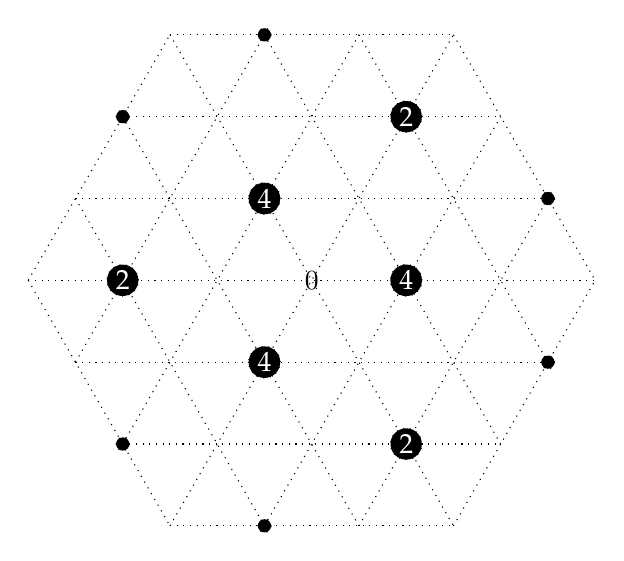
\begin{tikzpicture}[scale=1.2,dotted,bigger node/.style={fill=black,circle,draw,text=white,inner sep=1pt,font=\boldmath}]
  \draw (-3,0) -- (3,0);
  \draw (240:3) -- (60:3);
  \draw (120:3) -- (300:3);
  \draw (-3,0) -- (120:3);
  \draw (-3,0) -- (240:3);
  \draw (120:3) -- (60:3);
  \draw (240:3) -- (300:3);
  \draw (300:3) -- (3,0);
  \draw (60:3) -- (3,0);
  \draw (-2,{2*sin{60}}) -- (2,{2*sin{60}});
  \draw ({-2-cos{60}},{sin{60}}) -- ({2+cos{60}},{sin{60}});
  \draw (-2,{-2*sin{60}}) -- (2,{-2*sin{60}});
  \draw ({-2-cos{60}},{-sin{60}}) -- ({2+cos{60}},{-sin{60}});
  \draw (-2,{2*sin{60}}) -- (2,{2*sin{60}});
  \draw ({-2-cos{60}},{sin{60}}) -- ({-cos{60}},{-3*sin{60}});
  \draw ({-2},{2*sin{60}}) -- ({cos{60}},{-3*sin{60}});
  \draw ({-cos{60}},{3*sin{60}}) -- ({2},{-2*sin{60}});
  \draw ({cos{60}},{3*sin{60}}) -- ({2+cos{60}},{-sin{60}});
  \draw ({cos{60}},{-3*sin{60}}) -- ({2+cos{60}},{sin{60}});
  \draw ({-cos{60}},{-3*sin{60}}) -- ({2},{2*sin{60}});
  \draw ({-2},{-2*sin{60}}) -- ({cos{60}},{3*sin{60}});
  \draw ({-2-cos{60}},{-sin{60}}) -- ({-cos{60}},{3*sin{60}});
  \draw[fill] ({-cos{60}},{3*sin{60}}) circle [radius=0.07];
  \draw[fill] (-2,{2*sin{60}}) circle [radius=0.07];
  \node[bigger node] at (-2,0) {2};
  \draw[fill] ({-cos{60}},{-3*sin{60}}) circle [radius=0.07];
  \draw[fill] (-2,{-2*sin{60}}) circle [radius=0.07];
  \node[bigger node] at (1,{2*sin{60}}) {2};
  \node[bigger node] at (1,{-2*sin{60}}) {2};
  \draw[fill] (2.5,{sin{60}}) circle [radius=0.07];
  \draw[fill] (2.5,{-sin{60}}) circle [radius=0.07];
  \node[bigger node] at (120:1) {4};
  \node[bigger node] at (240:1) {4};
  \node[bigger node] at (0:1) {4};
  \node at (0,0) {$0$};
\end{tikzpicture}\end{center}}

\newcommand{\sltwoone}{\begin{center}
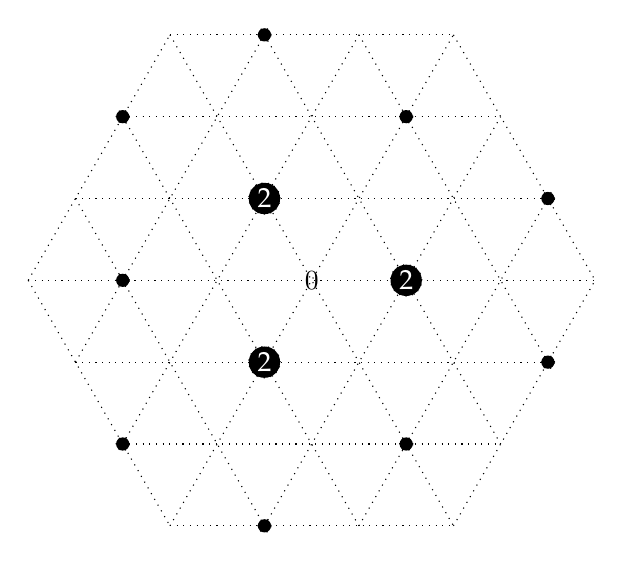
\begin{tikzpicture}[scale=1.2,dotted,bigger node/.style={fill=black,circle,draw,text=white,inner sep=1pt,font=\boldmath}]
  \draw (-3,0) -- (3,0);
  \draw (240:3) -- (60:3);
  \draw (120:3) -- (300:3);
  \draw (-3,0) -- (120:3);
  \draw (-3,0) -- (240:3);
  \draw (120:3) -- (60:3);
  \draw (240:3) -- (300:3);
  \draw (300:3) -- (3,0);
  \draw (60:3) -- (3,0);
  \draw (-2,{2*sin{60}}) -- (2,{2*sin{60}});
  \draw ({-2-cos{60}},{sin{60}}) -- ({2+cos{60}},{sin{60}});
  \draw (-2,{-2*sin{60}}) -- (2,{-2*sin{60}});
  \draw ({-2-cos{60}},{-sin{60}}) -- ({2+cos{60}},{-sin{60}});
  \draw (-2,{2*sin{60}}) -- (2,{2*sin{60}});
  \draw ({-2-cos{60}},{sin{60}}) -- ({-cos{60}},{-3*sin{60}});
  \draw ({-2},{2*sin{60}}) -- ({cos{60}},{-3*sin{60}});
  \draw ({-cos{60}},{3*sin{60}}) -- ({2},{-2*sin{60}});
  \draw ({cos{60}},{3*sin{60}}) -- ({2+cos{60}},{-sin{60}});
  \draw ({cos{60}},{-3*sin{60}}) -- ({2+cos{60}},{sin{60}});
  \draw ({-cos{60}},{-3*sin{60}}) -- ({2},{2*sin{60}});
  \draw ({-2},{-2*sin{60}}) -- ({cos{60}},{3*sin{60}});
  \draw ({-2-cos{60}},{-sin{60}}) -- ({-cos{60}},{3*sin{60}});
  \draw[fill] ({-cos{60}},{3*sin{60}}) circle [radius=0.07];
  \draw[fill] (-2,{2*sin{60}}) circle [radius=0.07];
  \draw[fill] (-2,0) circle [radius=0.07];
  \draw[fill] ({-cos{60}},{-3*sin{60}}) circle [radius=0.07];
  \draw[fill] (-2,{-2*sin{60}}) circle [radius=0.07];
  \draw[fill] (1,{2*sin{60}}) circle [radius=0.07];
  \draw[fill] (1,{-2*sin{60}}) circle [radius=0.07];
  \draw[fill] (2.5,{sin{60}}) circle [radius=0.07];
  \draw[fill] (2.5,{-sin{60}}) circle [radius=0.07];
  \node[bigger node] at (120:1) {2};
  \node[bigger node] at (240:1) {2};
  \node[bigger node] at (0:1) {2};
  \node at (0,0) {$0$};
\end{tikzpicture}\end{center}}

\newcommand{\slstdtensordual}{\begin{center}
\begin{tikzpicture}[scale=1.5,dotted,bigger node/.style={fill=black,circle,draw,text=white,inner sep=1pt,font=\boldmath}]
  \draw (240:2) -- (60:2);
  \draw (120:2) -- (300:2);
  \draw (60:2) -- (0:2);
  \draw (240:2) -- (180:2);
  \draw (180:2) -- (120:2);
  \draw (0:2) -- (300:2);
  \draw (120:2) -- (60:2);
  \draw (240:2) -- (300:2);
  \draw (180:2) -- (0:2);
  \draw (210:{2*sin{60}}) -- (330:{2*sin{60}});
  \draw (150:{2*sin{60}}) -- (30:{2*sin{60}});
  \draw (150:{2*sin{60}}) -- (270:{2*sin{60}});
  \draw (90:{2*sin{60}}) -- (330:{2*sin{60}});
  \draw (90:{2*sin{60}}) -- (210:{2*sin{60}});
  \draw (30:{2*sin{60}}) -- (270:{2*sin{60}});
  \draw[fill] (30:{2*sin{60}}) circle [radius=0.05];
  \draw[fill] (90:{2*sin{60}}) circle [radius=0.05];
  \draw[fill] (150:{2*sin{60}}) circle [radius=0.05];
  \draw[fill] (210:{2*sin{60}}) circle [radius=0.05];
  \draw[fill] (270:{2*sin{60}}) circle [radius=0.05];
  \draw[fill] (330:{2*sin{60}}) circle [radius=0.05];
  \draw[fill] (0,0) circle [radius=0.05];
  \node [above] at (0,0.3) {$0$};
  \node[bigger node] (0) at (0,0) {3};
  \node [right] at (30:{2*sin{60}}) {$L_1-L_3$};
  \node (1) at (30:{2*sin{60}}) {};
  \node [above] at (90:{2*sin{60}}) {$L_2-L_3$};
  \node (2) at (90:{2*sin{60}}) {};
  \node [left] at (150:{2*sin{60}}) {$L_2-L_1$};
  \node (3) at (150:{2*sin{60}}) {};
  \node [left] at (210:{2*sin{60}}) {$L_3-L_1$};
  \node (4) at (210:{2*sin{60}}) {};
  \node [below] at (270:{2*sin{60}}) {$L_3-L_2$};
  \node (5) at (270:{2*sin{60}}) {};
  \node [right] at (330:{2*sin{60}}) {$L_1-L_2$};
  \node (6) at (330:{2*sin{60}}) {};
\end{tikzpicture}\end{center}}

\newcommand{\meson}{\begin{center}
\begin{tikzpicture}[scale=1.5,dotted]
  \draw (240:2) -- (60:2);
  \draw (120:2) -- (300:2);
  \draw (60:2) -- (0:2);
  \draw (240:2) -- (180:2);
  \draw (180:2) -- (120:2);
  \draw (0:2) -- (300:2);
  \draw (120:2) -- (60:2);
  \draw (240:2) -- (300:2);
  \draw (180:2) -- (0:2);
  \draw (210:{2*sin{60}}) -- (330:{2*sin{60}});
  \draw (150:{2*sin{60}}) -- (30:{2*sin{60}});
  \draw (150:{2*sin{60}}) -- (270:{2*sin{60}});
  \draw (90:{2*sin{60}}) -- (330:{2*sin{60}});
  \draw (90:{2*sin{60}}) -- (210:{2*sin{60}});
  \draw (30:{2*sin{60}}) -- (270:{2*sin{60}});
  \draw[fill] (30:{2*sin{60}}) circle [radius=0.05];
  \draw[fill] (90:{2*sin{60}}) circle [radius=0.05];
  \draw[fill] (150:{2*sin{60}}) circle [radius=0.05];
  \draw[fill] (210:{2*sin{60}}) circle [radius=0.05];
  \draw[fill] (270:{2*sin{60}}) circle [radius=0.05];
  \draw[fill] (330:{2*sin{60}}) circle [radius=0.05];
  \draw[fill] (0,0) circle [radius=0.05];
  \node [above] at (0,0.1) {$0$};
  \node (0) at (0,0) {};
  \node [right] at (30:{2*sin{60}}) {$u\bar{s}=K^+$};
  \node (1) at (30:{2*sin{60}}) {};
  \node [above] at (90:{2*sin{60}}) {$d\bar{s}=K^0$};
  \node (2) at (90:{2*sin{60}}) {};
  \node [left] at (150:{2*sin{60}}) {$d\bar{u}=\pi^-$};
  \node (3) at (150:{2*sin{60}}) {};
  \node [left] at (210:{2*sin{60}}) {$s\bar{u}=K^-$};
  \node (4) at (210:{2*sin{60}}) {};
  \node [below] at (270:{2*sin{60}}) {$s\bar{d}=\bar{K}^0$};
  \node (5) at (270:{2*sin{60}}) {};
  \node [right] at (330:{2*sin{60}}) {$u\bar{d}=\pi^+$};
  \node (6) at (330:{2*sin{60}}) {};
\end{tikzpicture}\end{center}}

\newcommand{\baryon}{\begin{center}
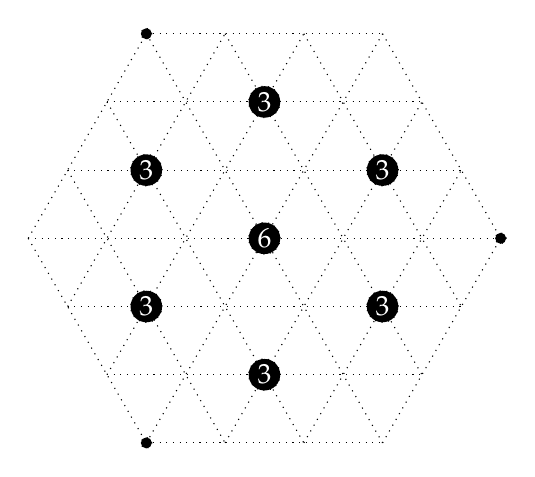
\begin{tikzpicture}[dotted,every node/.style={fill=black,circle,draw,text=white,inner sep=1pt,font=\boldmath}]
  \draw (-3,0) -- (3,0);
  \draw (240:3) -- (60:3);
  \draw (120:3) -- (300:3);
  \draw (-3,0) -- (120:3);
  \draw (-3,0) -- (240:3);
  \draw (120:3) -- (60:3);
  \draw (240:3) -- (300:3);
  \draw (300:3) -- (3,0);
  \draw (60:3) -- (3,0);
  \draw (-2,{2*sin{60}}) -- (2,{2*sin{60}});
  \draw ({-2-cos{60}},{sin{60}}) -- ({2+cos{60}},{sin{60}});
  \draw (-2,{-2*sin{60}}) -- (2,{-2*sin{60}});
  \draw ({-2-cos{60}},{-sin{60}}) -- ({2+cos{60}},{-sin{60}});
  \draw (-2,{2*sin{60}}) -- (2,{2*sin{60}});
  \draw ({-2-cos{60}},{sin{60}}) -- ({-cos{60}},{-3*sin{60}});
  \draw ({-2},{2*sin{60}}) -- ({cos{60}},{-3*sin{60}});
  \draw ({-cos{60}},{3*sin{60}}) -- ({2},{-2*sin{60}});
  \draw ({cos{60}},{3*sin{60}}) -- ({2+cos{60}},{-sin{60}});
  \draw ({cos{60}},{-3*sin{60}}) -- ({2+cos{60}},{sin{60}});
  \draw ({-cos{60}},{-3*sin{60}}) -- ({2},{2*sin{60}});
  \draw ({-2},{-2*sin{60}}) -- ({cos{60}},{3*sin{60}});
  \draw ({-2-cos{60}},{-sin{60}}) -- ({-cos{60}},{3*sin{60}});
  \draw[fill] ({-1.5},{3*sin{60}}) circle [radius=0.07];
  \node at (0,{2*sin{60}}) {3};
  \node at (1.5,{-sin{60}}) {3};
  \draw[fill] (-1.5,{-3*sin{60}}) circle [radius=0.07];
  \node at (0,{-2*sin{60}}) {3};
  \node at (1.5,{sin{60}}) {3};
  \draw[fill] (3,0) circle [radius=0.07];
  \node at (-1.5,{sin{60}}) {3};
  \node at (-1.5,{-sin{60}}) {3};
  \node at (0,0) {6};
\end{tikzpicture}\end{center}}


\newcommand{\decuplet}{\begin{center}
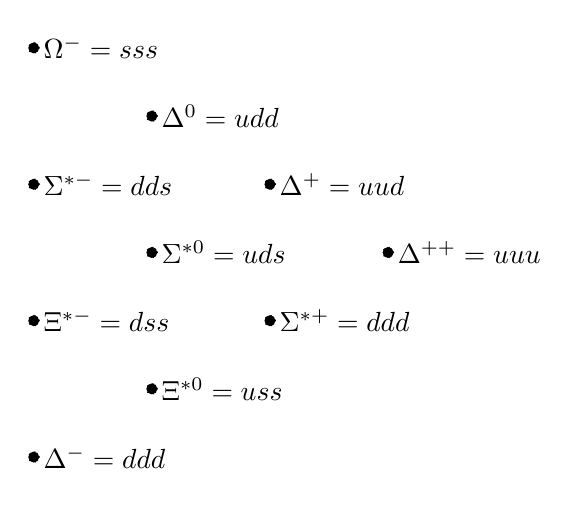
\begin{tikzpicture}[dotted]
  \draw[fill] ({-1.5},{3*sin{60}}) circle [radius=0.07];
  \draw[fill] (0,{2*sin{60}}) circle [radius=0.07];
  \draw[fill] (1.5,{-sin{60}}) circle [radius=0.07];
  \draw[fill] (-1.5,{-3*sin{60}}) circle [radius=0.07];
  \draw[fill] (0,{-2*sin{60}}) circle [radius=0.07];
  \draw[fill] (1.5,{sin{60}}) circle [radius=0.07];
  \draw[fill] (3,0) circle [radius=0.07];
  \draw[fill] (-1.5,{sin{60}}) circle [radius=0.07];
  \draw[fill] (-1.5,{-sin{60}}) circle [radius=0.07];
  \draw[fill] (0,0) circle [radius=0.07];
  \node [right] at (3,0) {$\Delta^{++}=uuu$};
  \node [right] at (0,0) {$\Sigma^{*0}=uds$};
  \node [right] at (-1.5,{-3*sin{60}}) {$\Delta^{-}=ddd$};
  \node [right] at (-1.5,{3*sin{60}}) {$\Omega^{-}=sss$};
  \node [right] at (0,{2*sin{60}}) {$\Delta^{0}=udd$};
  \node [right] at (1.5,{sin{60}}) {$\Delta^{+}=uud$};
  \node [right] at (0,{-2*sin{60}}) {$\Xi^{*0}=uss$};
  \node [right] at (-1.5,{sin{60}}) {$\Sigma^{*-}=dds$};
  \node [right] at (-1.5,{-sin{60}}) {$\Xi^{*-}=dss$};
  \node [right] at (1.5,{-sin{60}}) {$\Sigma^{*+}=ddd$};
\end{tikzpicture}\end{center}}

\newcommand{\baryonoctet}{\begin{center}
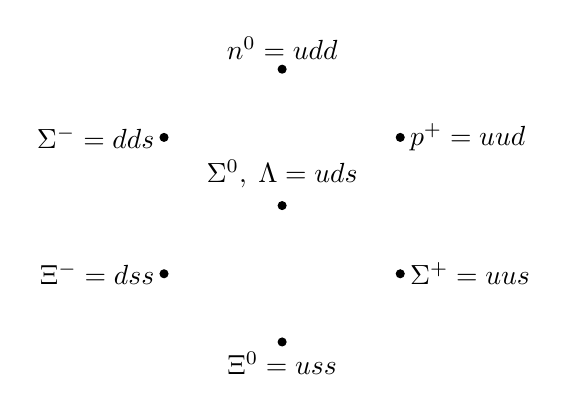
\begin{tikzpicture}
  \draw[fill] (30:{2*sin{60}}) circle [radius=0.05];
  \draw[fill] (90:{2*sin{60}}) circle [radius=0.05];
  \draw[fill] (150:{2*sin{60}}) circle [radius=0.05];
  \draw[fill] (210:{2*sin{60}}) circle [radius=0.05];
  \draw[fill] (270:{2*sin{60}}) circle [radius=0.05];
  \draw[fill] (330:{2*sin{60}}) circle [radius=0.05];
  \draw[fill] (0,0) circle [radius=0.05];
  \node [above] at (0,0.1) {$\Sigma^0,\ \Lambda=uds$};
  \node (0) at (0,0) {};
  \node [right] at (30:{2*sin{60}}) {$p^+=uud$};
  \node (1) at (30:{2*sin{60}}) {};
  \node [above] at (90:{2*sin{60}}) {$n^0=udd$};
  \node (2) at (90:{2*sin{60}}) {};
  \node [left] at (150:{2*sin{60}}) {$\Sigma^-=dds$};
  \node (3) at (150:{2*sin{60}}) {};
  \node [left] at (210:{2*sin{60}}) {$\Xi^-=dss$};
  \node (4) at (210:{2*sin{60}}) {};
  \node [below] at (270:{2*sin{60}}) {$\Xi^0=uss$};
  \node (5) at (270:{2*sin{60}}) {};
  \node [right] at (330:{2*sin{60}}) {$\Sigma^+=uus$};
  \node (6) at (330:{2*sin{60}}) {};
\end{tikzpicture}\end{center}}

% Some more pictures for SU(3)

\newcommand{\slhex}{\begin{center}
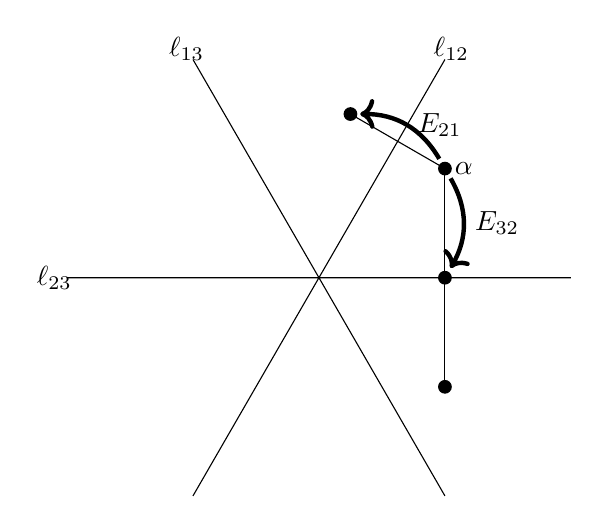
\begin{tikzpicture}[scale=0.8]
  \draw
     (-4,0) -- (4,0)
     (240:4) -- (60:4)
     (120:4) -- (-60:4);
  \node at (-4.2,0) {$\ell_{23}$};
  \node at (60:4.2) {$\ell_{12}$};
  \node at (120:4.2) {$\ell_{13}$};
  \node at (2.3,1.73205080757) {$\alpha$};
  \node (1) at (2,1.73205080757) {};
  \node (2) at (0.5,2.59807621135) {};
  \node (3) at (2,0) {};
  \draw [fill] (2,1.73205080757) circle [radius=0.1];
  \draw [fill] (2,-1.73205080757) circle [radius=0.1];
  \draw [fill] (2,0) circle [radius=0.1];
  \draw [fill] (0.5,2.59807621135) circle [radius=0.1];
  \draw (2,1.73205080757) -- (2,-1.73205080757);
  \draw (2,1.73205080757) -- (0.5,2.59807621135);
  \path[ultra thick,solid,->] 
  (1) edge [bend right] node [right] {$E_{21}$} (2)
  (1) edge [bend left] node [right] {$E_{32}$} (3);
\end{tikzpicture}
\end{center}}

\newcommand{\gtwoadj}{\begin{center}
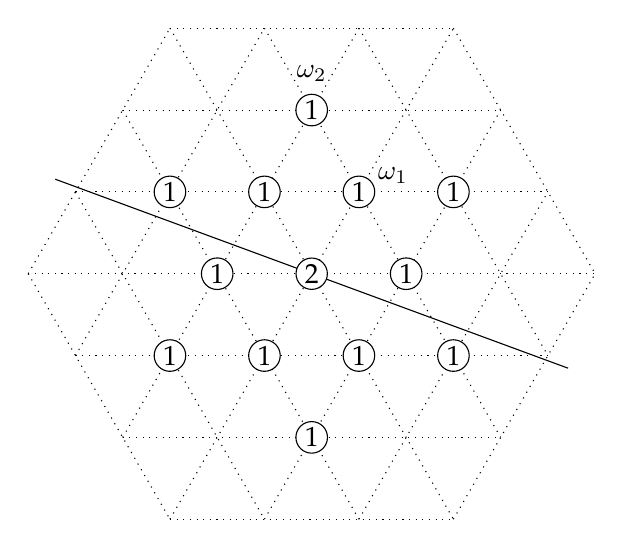
\begin{tikzpicture}[scale=1.2,dotted,bigger node/.style={fill=white,solid,circle,draw,text=black,inner sep=1pt,font=\boldmath}]
  \draw (-3,0) -- (3,0);
  \draw (240:3) -- (60:3);
  \draw (120:3) -- (300:3);
  \draw (-3,0) -- (120:3);
  \draw (-3,0) -- (240:3);
  \draw (120:3) -- (60:3);
  \draw (240:3) -- (300:3);
  \draw (300:3) -- (3,0);
  \draw (60:3) -- (3,0);
  \draw (-2,{2*sin{60}}) -- (2,{2*sin{60}});
  \draw ({-2-cos{60}},{sin{60}}) -- ({2+cos{60}},{sin{60}});
  \draw (-2,{-2*sin{60}}) -- (2,{-2*sin{60}});
  \draw ({-2-cos{60}},{-sin{60}}) -- ({2+cos{60}},{-sin{60}});
  \draw (-2,{2*sin{60}}) -- (2,{2*sin{60}});
  \draw ({-2-cos{60}},{sin{60}}) -- ({-cos{60}},{-3*sin{60}});
  \draw ({-2},{2*sin{60}}) -- ({cos{60}},{-3*sin{60}});
  \draw ({-cos{60}},{3*sin{60}}) -- ({2},{-2*sin{60}});
  \draw ({cos{60}},{3*sin{60}}) -- ({2+cos{60}},{-sin{60}});
  \draw ({cos{60}},{-3*sin{60}}) -- ({2+cos{60}},{sin{60}});
  \draw ({-cos{60}},{-3*sin{60}}) -- ({2},{2*sin{60}});
  \draw ({-2},{-2*sin{60}}) -- ({cos{60}},{3*sin{60}});
  \draw ({-2-cos{60}},{-sin{60}}) -- ({-cos{60}},{3*sin{60}});
  \draw [solid] (-2.7135,1) -- (2.7135,-1);

  \node[bigger node] at (0,0) {2};
  \node[bigger node] at (30:1.73205080757) {1};
  \node[bigger node] at (90:1.73205080757) {1};
  \node[bigger node] at (150:1.73205080757) {1};
  \node[bigger node] at (210:1.73205080757) {1};
  \node[bigger node] at (270:1.73205080757) {1};
  \node[bigger node] at (330:1.73205080757) {1};
  \node[above] at (90:1.93205080757) {$\omega_2$};
  \node[bigger node] at (0:1) {1};
  \node[bigger node] at (60:1) {1};
  \node[bigger node] at (120:1) {1};
  \node[bigger node] at (180:1) {1};
  \node[bigger node] at (240:1) {1};
  \node[bigger node] at (300:1) {1};
  \node[right] at (60:1.2) {$\omega_1$};
\end{tikzpicture}\end{center}}

\newcommand{\gtwoadjpos}{\begin{center}
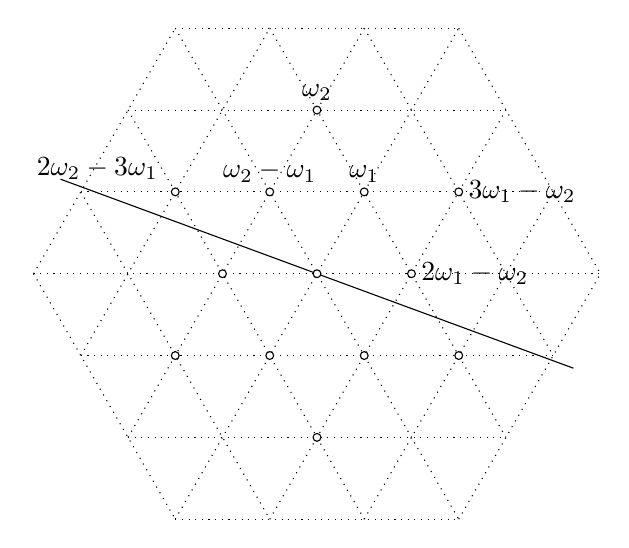
\begin{tikzpicture}[scale=1.2,dotted,bigger node/.style={fill=white,solid,circle,draw,text=black,inner sep=1pt,font=\boldmath}]
  \draw (-3,0) -- (3,0);
  \draw (240:3) -- (60:3);
  \draw (120:3) -- (300:3);
  \draw (-3,0) -- (120:3);
  \draw (-3,0) -- (240:3);
  \draw (120:3) -- (60:3);
  \draw (240:3) -- (300:3);
  \draw (300:3) -- (3,0);
  \draw (60:3) -- (3,0);
  \draw (-2,{2*sin{60}}) -- (2,{2*sin{60}});
  \draw ({-2-cos{60}},{sin{60}}) -- ({2+cos{60}},{sin{60}});
  \draw (-2,{-2*sin{60}}) -- (2,{-2*sin{60}});
  \draw ({-2-cos{60}},{-sin{60}}) -- ({2+cos{60}},{-sin{60}});
  \draw (-2,{2*sin{60}}) -- (2,{2*sin{60}});
  \draw ({-2-cos{60}},{sin{60}}) -- ({-cos{60}},{-3*sin{60}});
  \draw ({-2},{2*sin{60}}) -- ({cos{60}},{-3*sin{60}});
  \draw ({-cos{60}},{3*sin{60}}) -- ({2},{-2*sin{60}});
  \draw ({cos{60}},{3*sin{60}}) -- ({2+cos{60}},{-sin{60}});
  \draw ({cos{60}},{-3*sin{60}}) -- ({2+cos{60}},{sin{60}});
  \draw ({-cos{60}},{-3*sin{60}}) -- ({2},{2*sin{60}});
  \draw ({-2},{-2*sin{60}}) -- ({cos{60}},{3*sin{60}});
  \draw ({-2-cos{60}},{-sin{60}}) -- ({-cos{60}},{3*sin{60}});
  \draw [solid] (-2.7135,1) -- (2.7135,-1);

  \node[bigger node] at (0,0) {};
  \node[bigger node] at (30:1.73205080757) {};
  \node[bigger node] at (90:1.73205080757) {};
  \node[bigger node] at (150:1.73205080757) {};
  \node[bigger node] at (210:1.73205080757) {};
  \node[bigger node] at (270:1.73205080757) {};
  \node[bigger node] at (330:1.73205080757) {};
  \node[bigger node] at (0:1) {};
  \node[bigger node] at (60:1) {};
  \node[bigger node] at (120:1) {};
  \node[bigger node] at (180:1) {};
  \node[bigger node] at (240:1) {};
  \node[bigger node] at (300:1) {};

  \node[right] at (30:1.73205080757) {$3\omega_1-\omega_2$};
  \node[above] at (90:1.73205080757) {$\omega_2$};
  \node[left] at (145:1.93205080757) {$2\omega_2-3\omega_1$};
  \node[right] at (0:1) {$2\omega_1-\omega_2$};
  \node[above] at (60:1) {$\omega_1$};
  \node[above] at (120:1) {$\omega_2-\omega_1$};
\end{tikzpicture}\end{center}}

\newcommand{\gtwolambdaonezero}{\begin{center}
\begin{tikzpicture}[scale=1.2,dotted,bigger node/.style={fill=white,solid,circle,draw,text=black,inner sep=1pt,font=\boldmath}]
  \draw (-3,0) -- (3,0);
  \draw (240:3) -- (60:3);
  \draw (120:3) -- (300:3);
  \draw (-3,0) -- (120:3);
  \draw (-3,0) -- (240:3);
  \draw (120:3) -- (60:3);
  \draw (240:3) -- (300:3);
  \draw (300:3) -- (3,0);
  \draw (60:3) -- (3,0);
  \draw (-2,{2*sin{60}}) -- (2,{2*sin{60}});
  \draw ({-2-cos{60}},{sin{60}}) -- ({2+cos{60}},{sin{60}});
  \draw (-2,{-2*sin{60}}) -- (2,{-2*sin{60}});
  \draw ({-2-cos{60}},{-sin{60}}) -- ({2+cos{60}},{-sin{60}});
  \draw (-2,{2*sin{60}}) -- (2,{2*sin{60}});
  \draw ({-2-cos{60}},{sin{60}}) -- ({-cos{60}},{-3*sin{60}});
  \draw ({-2},{2*sin{60}}) -- ({cos{60}},{-3*sin{60}});
  \draw ({-cos{60}},{3*sin{60}}) -- ({2},{-2*sin{60}});
  \draw ({cos{60}},{3*sin{60}}) -- ({2+cos{60}},{-sin{60}});
  \draw ({cos{60}},{-3*sin{60}}) -- ({2+cos{60}},{sin{60}});
  \draw ({-cos{60}},{-3*sin{60}}) -- ({2},{2*sin{60}});
  \draw ({-2},{-2*sin{60}}) -- ({cos{60}},{3*sin{60}});
  \draw ({-2-cos{60}},{-sin{60}}) -- ({-cos{60}},{3*sin{60}});

  \node[bigger node] at (0,0) {};
  \node[bigger node] at (0:1) {};
  \node[bigger node] at (60:1) {};
  \node[bigger node] at (120:1) {};
  \node[bigger node] at (180:1) {};
  \node[bigger node] at (240:1) {};
  \node[bigger node] at (300:1) {};
  \node[right] at (60:1.2) {$\omega_1$};
\end{tikzpicture}\end{center}}

\newcommand{\gtwolambdatwozero}{\begin{center}
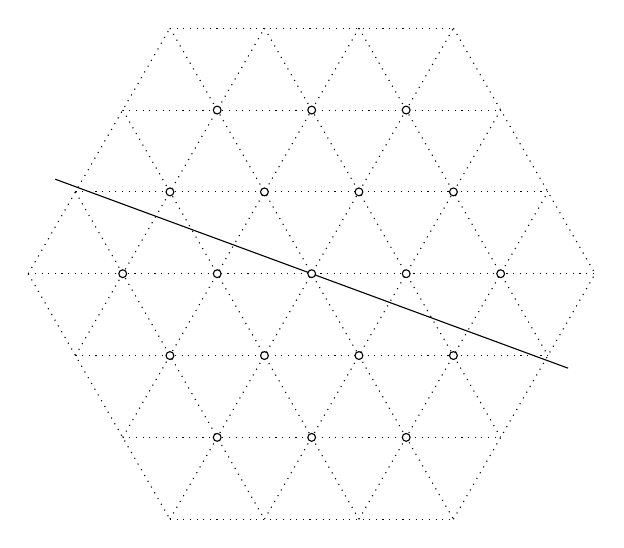
\begin{tikzpicture}[scale=1.2,dotted,bigger node/.style={fill=white,solid,circle,draw,text=black,inner sep=1pt,font=\boldmath}]
  \draw (-3,0) -- (3,0);
  \draw (240:3) -- (60:3);
  \draw (120:3) -- (300:3);
  \draw (-3,0) -- (120:3);
  \draw (-3,0) -- (240:3);
  \draw (120:3) -- (60:3);
  \draw (240:3) -- (300:3);
  \draw (300:3) -- (3,0);
  \draw (60:3) -- (3,0);
  \draw (-2,{2*sin{60}}) -- (2,{2*sin{60}});
  \draw ({-2-cos{60}},{sin{60}}) -- ({2+cos{60}},{sin{60}});
  \draw (-2,{-2*sin{60}}) -- (2,{-2*sin{60}});
  \draw ({-2-cos{60}},{-sin{60}}) -- ({2+cos{60}},{-sin{60}});
  \draw (-2,{2*sin{60}}) -- (2,{2*sin{60}});
  \draw ({-2-cos{60}},{sin{60}}) -- ({-cos{60}},{-3*sin{60}});
  \draw ({-2},{2*sin{60}}) -- ({cos{60}},{-3*sin{60}});
  \draw ({-cos{60}},{3*sin{60}}) -- ({2},{-2*sin{60}});
  \draw ({cos{60}},{3*sin{60}}) -- ({2+cos{60}},{-sin{60}});
  \draw ({cos{60}},{-3*sin{60}}) -- ({2+cos{60}},{sin{60}});
  \draw ({-cos{60}},{-3*sin{60}}) -- ({2},{2*sin{60}});
  \draw ({-2},{-2*sin{60}}) -- ({cos{60}},{3*sin{60}});
  \draw ({-2-cos{60}},{-sin{60}}) -- ({-cos{60}},{3*sin{60}});
  \draw [solid] (-2.7135,1) -- (2.7135,-1);

  \node[bigger node] at (0,0) {};
  \node[bigger node] at (30:1.73205080757) {};
  \node[bigger node] at (90:1.73205080757) {};
  \node[bigger node] at (150:1.73205080757) {};
  \node[bigger node] at (210:1.73205080757) {};
  \node[bigger node] at (270:1.73205080757) {};
  \node[bigger node] at (330:1.73205080757) {};
  \node[bigger node] at (0:1) {};
  \node[bigger node] at (60:1) {};
  \node[bigger node] at (120:1) {};
  \node[bigger node] at (180:1) {};
  \node[bigger node] at (240:1) {};
  \node[bigger node] at (300:1) {};
  \node[bigger node] at (0:2) {};
  \node[bigger node] at (60:2) {};
  \node[bigger node] at (120:2) {};
  \node[bigger node] at (180:2) {};
  \node[bigger node] at (240:2) {};
  \node[bigger node] at (300:2) {};
\end{tikzpicture}\end{center}}

\newcommand{\gtwolabel}{\begin{center}
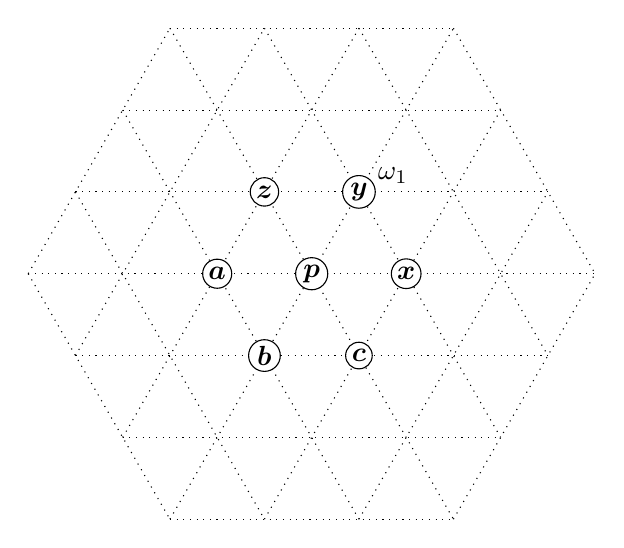
\begin{tikzpicture}[scale=1.2,dotted,bigger node/.style={fill=white,solid,circle,draw,text=black,inner sep=1pt,font=\boldmath}]
  \draw (-3,0) -- (3,0);
  \draw (240:3) -- (60:3);
  \draw (120:3) -- (300:3);
  \draw (-3,0) -- (120:3);
  \draw (-3,0) -- (240:3);
  \draw (120:3) -- (60:3);
  \draw (240:3) -- (300:3);
  \draw (300:3) -- (3,0);
  \draw (60:3) -- (3,0);
  \draw (-2,{2*sin{60}}) -- (2,{2*sin{60}});
  \draw ({-2-cos{60}},{sin{60}}) -- ({2+cos{60}},{sin{60}});
  \draw (-2,{-2*sin{60}}) -- (2,{-2*sin{60}});
  \draw ({-2-cos{60}},{-sin{60}}) -- ({2+cos{60}},{-sin{60}});
  \draw (-2,{2*sin{60}}) -- (2,{2*sin{60}});
  \draw ({-2-cos{60}},{sin{60}}) -- ({-cos{60}},{-3*sin{60}});
  \draw ({-2},{2*sin{60}}) -- ({cos{60}},{-3*sin{60}});
  \draw ({-cos{60}},{3*sin{60}}) -- ({2},{-2*sin{60}});
  \draw ({cos{60}},{3*sin{60}}) -- ({2+cos{60}},{-sin{60}});
  \draw ({cos{60}},{-3*sin{60}}) -- ({2+cos{60}},{sin{60}});
  \draw ({-cos{60}},{-3*sin{60}}) -- ({2},{2*sin{60}});
  \draw ({-2},{-2*sin{60}}) -- ({cos{60}},{3*sin{60}});
  \draw ({-2-cos{60}},{-sin{60}}) -- ({-cos{60}},{3*sin{60}});

  \node[bigger node] at (0,0) {$p$};
  \node[bigger node] at (0:1) {$x$};
  \node[bigger node] at (60:1) {$y$};
  \node[bigger node] at (120:1) {$z$};
  \node[bigger node] at (180:1) {$a$};
  \node[bigger node] at (240:1) {$b$};
  \node[bigger node] at (300:1) {$c$};
  \node[right] at (60:1.2) {$\omega_1$};
\end{tikzpicture}\end{center}}

\newcommand{\gtwolabeltwo}{\begin{center}
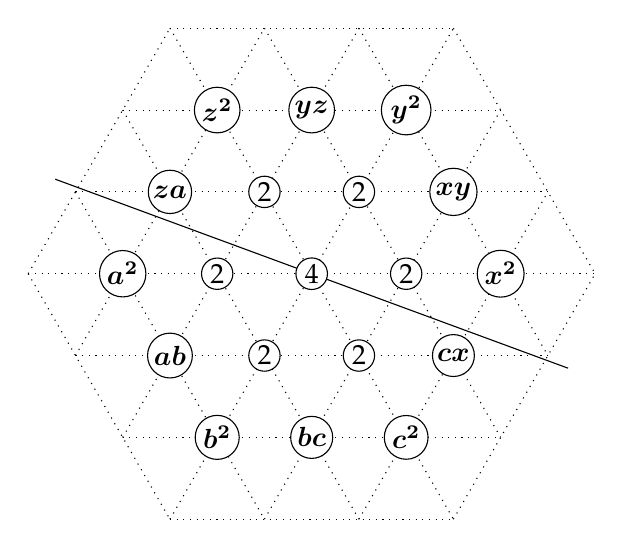
\begin{tikzpicture}[scale=1.2,dotted,bigger node/.style={fill=white,solid,circle,draw,text=black,inner sep=1pt,font=\boldmath}]
  \draw (-3,0) -- (3,0);
  \draw (240:3) -- (60:3);
  \draw (120:3) -- (300:3);
  \draw (-3,0) -- (120:3);
  \draw (-3,0) -- (240:3);
  \draw (120:3) -- (60:3);
  \draw (240:3) -- (300:3);
  \draw (300:3) -- (3,0);
  \draw (60:3) -- (3,0);
  \draw (-2,{2*sin{60}}) -- (2,{2*sin{60}});
  \draw ({-2-cos{60}},{sin{60}}) -- ({2+cos{60}},{sin{60}});
  \draw (-2,{-2*sin{60}}) -- (2,{-2*sin{60}});
  \draw ({-2-cos{60}},{-sin{60}}) -- ({2+cos{60}},{-sin{60}});
  \draw (-2,{2*sin{60}}) -- (2,{2*sin{60}});
  \draw ({-2-cos{60}},{sin{60}}) -- ({-cos{60}},{-3*sin{60}});
  \draw ({-2},{2*sin{60}}) -- ({cos{60}},{-3*sin{60}});
  \draw ({-cos{60}},{3*sin{60}}) -- ({2},{-2*sin{60}});
  \draw ({cos{60}},{3*sin{60}}) -- ({2+cos{60}},{-sin{60}});
  \draw ({cos{60}},{-3*sin{60}}) -- ({2+cos{60}},{sin{60}});
  \draw ({-cos{60}},{-3*sin{60}}) -- ({2},{2*sin{60}});
  \draw ({-2},{-2*sin{60}}) -- ({cos{60}},{3*sin{60}});
  \draw ({-2-cos{60}},{-sin{60}}) -- ({-cos{60}},{3*sin{60}});
  \draw [solid] (-2.7135,1) -- (2.7135,-1);

  \node[bigger node] at (0,0) {4};
  \node[bigger node] at (30:1.73205080757) {$xy$};
  \node[bigger node] at (90:1.73205080757) {$yz$};
  \node[bigger node] at (150:1.73205080757) {$za$};
  \node[bigger node] at (210:1.73205080757) {$ab$};
  \node[bigger node] at (270:1.73205080757) {$bc$};
  \node[bigger node] at (330:1.73205080757) {$cx$};
  \node[bigger node] at (0:1) {2};
  \node[bigger node] at (60:1) {2};
  \node[bigger node] at (120:1) {2};
  \node[bigger node] at (180:1) {2};
  \node[bigger node] at (240:1) {2};
  \node[bigger node] at (300:1) {2};
  \node[bigger node] at (0:2) {$x^2$};
  \node[bigger node] at (60:2) {$y^2$};
  \node[bigger node] at (120:2) {$z^2$};
  \node[bigger node] at (180:2) {$a^2$};
  \node[bigger node] at (240:2) {$b^2$};
  \node[bigger node] at (300:2) {$c^2$};
\end{tikzpicture}\end{center}}

\newcommand{\gtwolambdathree}{\begin{center}
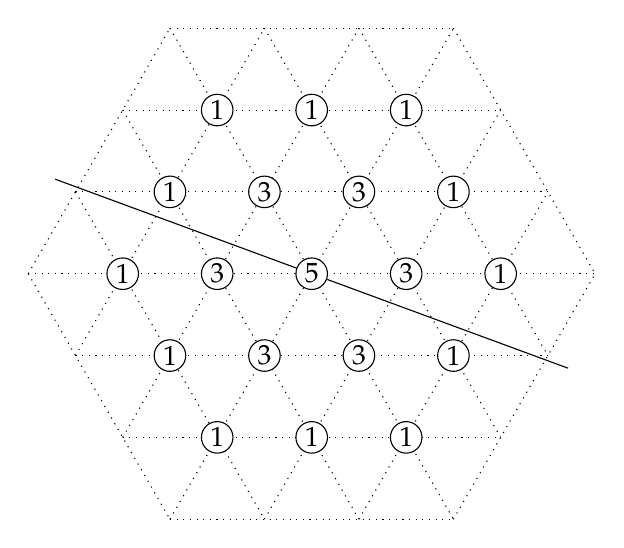
\begin{tikzpicture}[scale=1.2,dotted,bigger node/.style={fill=white,solid,circle,draw,text=black,inner sep=1pt,font=\boldmath}]
  \draw (-3,0) -- (3,0);
  \draw (240:3) -- (60:3);
  \draw (120:3) -- (300:3);
  \draw (-3,0) -- (120:3);
  \draw (-3,0) -- (240:3);
  \draw (120:3) -- (60:3);
  \draw (240:3) -- (300:3);
  \draw (300:3) -- (3,0);
  \draw (60:3) -- (3,0);
  \draw (-2,{2*sin{60}}) -- (2,{2*sin{60}});
  \draw ({-2-cos{60}},{sin{60}}) -- ({2+cos{60}},{sin{60}});
  \draw (-2,{-2*sin{60}}) -- (2,{-2*sin{60}});
  \draw ({-2-cos{60}},{-sin{60}}) -- ({2+cos{60}},{-sin{60}});
  \draw (-2,{2*sin{60}}) -- (2,{2*sin{60}});
  \draw ({-2-cos{60}},{sin{60}}) -- ({-cos{60}},{-3*sin{60}});
  \draw ({-2},{2*sin{60}}) -- ({cos{60}},{-3*sin{60}});
  \draw ({-cos{60}},{3*sin{60}}) -- ({2},{-2*sin{60}});
  \draw ({cos{60}},{3*sin{60}}) -- ({2+cos{60}},{-sin{60}});
  \draw ({cos{60}},{-3*sin{60}}) -- ({2+cos{60}},{sin{60}});
  \draw ({-cos{60}},{-3*sin{60}}) -- ({2},{2*sin{60}});
  \draw ({-2},{-2*sin{60}}) -- ({cos{60}},{3*sin{60}});
  \draw ({-2-cos{60}},{-sin{60}}) -- ({-cos{60}},{3*sin{60}});
  \draw [solid] (-2.7135,1) -- (2.7135,-1);

  \node[bigger node] at (0,0) {5};
  \node[bigger node] at (30:1.73205080757) {1};
  \node[bigger node] at (90:1.73205080757) {1};
  \node[bigger node] at (150:1.73205080757) {1};
  \node[bigger node] at (210:1.73205080757) {1};
  \node[bigger node] at (270:1.73205080757) {1};
  \node[bigger node] at (330:1.73205080757) {1};
  \node[bigger node] at (0:1) {3};
  \node[bigger node] at (60:1) {3};
  \node[bigger node] at (120:1) {3};
  \node[bigger node] at (180:1) {3};
  \node[bigger node] at (240:1) {3};
  \node[bigger node] at (300:1) {3};
  \node[bigger node] at (0:2) {1};
  \node[bigger node] at (60:2) {1};
  \node[bigger node] at (120:2) {1};
  \node[bigger node] at (180:2) {1};
  \node[bigger node] at (240:2) {1};
  \node[bigger node] at (300:2) {1};
\end{tikzpicture}\end{center}}

\newcommand{\gtwodynkin}{\begin{center}
  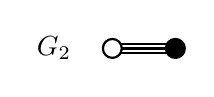
\begin{tikzpicture}[scale=.4]
    \draw (-1,0) node[anchor=east]  {$G_2$};
    \draw[thick] (0 ,0) circle (.3 cm);
    \draw[thick,fill=black] (2 cm,0) circle (.3 cm);
    \draw[thick] (30: 3mm) -- +(1.5 cm, 0);
    \draw[thick] (0: 3 mm) -- +(1.4 cm, 0);
    \draw[thick] (-30: 3 mm) -- +(1.5 cm, 0);
  \end{tikzpicture}
\end{center}}



%%% Local Variables: 
%%% mode: latex
%%% TeX-master: "master"
%%% End: 

\newcommand{\HRule}{\rule{\linewidth}{0.5mm}}

\newcommand{\dd}[2]{\frac{d #1}{d #2}}
\newcommand{\pd}[2]{\frac{\partial #1}{\partial #2}}
\newcommand{\m}{\mathcal}
\newcommand{\BB}{\mathbf}
\newcommand{\CC}{\mathbf{C}}
\newcommand{\RR}{\mathbf{R}}
\newcommand{\QQ}{\mathbf{Q}}
\newcommand{\PP}{\mathbf{P}}
\newcommand{\ZZ}{\mathbf{Z}}
\newcommand{\HH}{\mathbf{H}}
\newcommand{\KK}{\mathbf{K}}
\newcommand{\OP}{\operatorname}
\newcommand{\op}{\operatorname}
\newcommand{\into}{\hookrightarrow}
\newcommand{\Hom}{\mathrm{Hom}}
\newcommand{\End}{\OP{End}}
\newcommand{\ad}{\OP{ad}}
\newcommand{\Ad}{\OP{Ad}}
\newcommand{\Sym}{\OP{Sym}}
\newcommand{\hh}{\mathfrak{h}}
\newcommand{\id}{\mathrm{id}}
\newcommand{\diag}{\mathrm{diag}}
\newcommand{\Tr}{\mathrm{Tr}}
\newcommand{\kk}{\mathbf{k}}
\newcommand{\vrow}[2]{\left(\begin{array}{cc}#1 & #2\end{array}\right)}
\newcommand{\vcol}[2]{\left(\begin{array}{c}#1\\ #2\end{array}\right)}
\newcommand{\vrot}[3]{\left(\begin{array}{ccc}#1 & #2 & #3\end{array}\right)}
\newcommand{\vcot}[3]{\left(\begin{array}{c}#1\\ #2\\ #3\end{array}\right)}
\newcommand{\matr}[4]{\left(\begin{array}{cc}#1 & #2\\ #3 & #4\end{array}\right)}
\newcommand{\Diag}[3]{\left(\begin{array}{ccc}#1 & 0 & 0\\0 & #2 & 0\\0 & 0 & #3\end{array}\right)}
\newcommand{\mats}[4]{\left(\begin{array}{ccc}#1 & \cdots & #2\\ \vdots & \ddots & \vdots \\ #3 & \cdots & #4\end{array}\right)}
\newcommand{\matt}[9]{\left(\begin{array}{ccc}#1 & #2 & #3\\#4 & #5 & #6\\#7 & #8 & #9\end{array}\right)}
\newcommand{\MAT}[4]{\left(\begin{array}{ccc}#1 & \cdots & #2\\ \vdots & \ddots & \vdots\\ #3 & \cdots & #4\end{array}\right)}
\newcommand{\MATR}[9]{\left(\begin{array}{cccc}#1 & #2 & \cdots & #3\\ #4 & #5 &  & #6\\ \vdots & &\ddots &\vdots\\ #7 & #8 & \cdots & #9\\\end{array}\right)}

\setcounter{secnumdepth}{3}

\newtheorem{thm}{Theorem}[section]
\newtheorem{thmalpha}{Theorem}
\newtheorem{lma}[thm]{Lemma}
\newtheorem{lmaclub}[thm]{$\clubsuit$ Lemma}
\newtheorem{prp}[thm]{Proposition}
\newtheorem{cor}[thm]{Corollary}

\theoremstyle{definition}

\newtheorem{dfn}[thm]{Definition}
\newtheorem{exm}[thm]{Example}
\newtheorem{exmclub}[thm]{$\clubsuit$ Example}
\newtheorem{obs}[thm]{Observation}
\newtheorem*{clm}{Claim}

\newtheoremstyle{check}% name of the style to be used
  {}% measure of space to leave above the theorem. E.g.: 3pt
  {}% measure of space to leave below the theorem. E.g.: 3pt
  {}% name of font to use in the body of the theorem
  {}% measure of space to indent
  {\bf}% name of head font
  {!}% punctuation between head and body
  { }% space after theorem head; " " = normal interword space
  {}% manually specify head
\theoremstyle{check}
\newtheorem*{chk}{Check}

\theoremstyle{remark}
\newtheorem{rmk}[thm]{Remark}

\setcounter{tocdepth}{1}

\newtheoremstyle{TheoremNum}
    {\topsep}{\topsep}              %%% space between body and thm
    {\itshape}                      %%% Thm body font
    {}                              %%% Indent amount (empty = no indent)
    {\bfseries}                     %%% Thm head font
    {.}                             %%% Punctuation after thm head
    { }                             %%% Space after thm head
    {\thmname{#1}\thmnote{ \bfseries #3}}%%% Thm head spec
\theoremstyle{TheoremNum}

\begingroup 
\makeatletter 
\@for\theoremstyle:=definition,remark,plain,check,TheoremNum\do{% 
\expandafter\g@addto@macro\csname th@\theoremstyle\endcsname{% 
\addtolength\thm@preskip\parskip 
}% 
} 
\endgroup 

\renewcommand*{\thethmalpha}{\Alph{thmalpha}}

% Next bit redefines the proof environment so it's more like Arnold's book ``Mathematical methods of classical mechanics''.

\makeatletter \renewenvironment{proof}[1][\proofname]
{\par\pushQED{\qed}\normalfont\topsep6\p@\@plus6\p@\relax\begin{list}{}{\rightmargin=2em\leftmargin=2em}\item[\hskip\labelsep\bfseries#1\@addpunct{.}]\ignorespaces\footnotesize}{\popQED\end{list}\@endpefalse}
\makeatother

\title{Lie groups and Lie algebras}
\author{Jonny Evans}

\begin{document}

\maketitle

\section{Introduction}

To the students, past, present and future, who have/are/will taken/taking/take this course and to those interested parties who just read the notes and gave me feedback: thank you for providing the background level of enthusiasm, pedantry and general confusion needed to force me to improve these notes. All comments and corrections are very welcome.

\subsection{What is a representation?}

\begin{dfn}
A representation $\rho$ of a group $G$ on an $n$-dimensional vector space $V$ over a field $\kk$ is an assignment of a $\kk$-linear map $\rho(g)\colon V\to V$ to each group element $g$ such that
\begin{itemize}
\item $\rho(gh)=\rho(g)\rho(h)$
\item $\rho(1_G)=1_V$.
\end{itemize}
\end{dfn}

Here are some equivalent definitions. A representation is...

\begin{enumerate}
\item ...an assignment of an $n$-by-$n$ matrix $\rho(g)$ to each group element $g$ such that $\rho(gh)=\rho(g)\rho(h)$ (i.e. the matrices multiply together like the group elements they represent). This is clearly the same as the previous definition once you have picked a basis of $V$ to identify linear maps with matrices;
\item ...a homomorphism $\rho\colon G\to GL(V)$. The multiplicativity condition is now hiding in the definition of homomorphism, which requires $\rho(gh)=\rho(g)\rho(h)$;
\item ...an action of $G$ on $V$ by linear maps. In other words an action $\tilde{\rho}\colon G\times V\to V$ such that, for each $g\in G$, the map $\rho(g)\colon V\to V$ defined by $\rho(g)(v)=\tilde{\rho}(g,v)$ is linear. The multiplicativity condition is now hiding in the definition of an action, which requires $\tilde{\rho}(gh,v)=\tilde{\rho}(g,\tilde{\rho}(h,v))$.
\end{enumerate}

You should internalise these points of view as being all the same: I will switch between them. More confusingly still, I will sometimes say ``let $V$ be a representation of $G$'' or ``consider the action $\rho$ of $G$ on $V$''. This is the only warning you'll get, so don't be confused.

\subsection{Why do we care?}

Why do we study representations? How do representations arise in the real world (of mathematics)? Here is a motivating example.

\begin{exm}[Invariant theory for binary quadratic forms] For simplicity, let's work over $\CC$. A {\em binary quadratic form} is an expression $ax^2+bxy+cy^2$ in two variables. One can add and subtract quadratic forms and rescale them by a real number, so they form a vector space. Another way to write a quadratic form is:
\[ax^2+bxy+cy^2=\vrow{x}{y}\matr{a}{b/2}{b/2}{c}\vcol{x}{y}=:\vec{x}^TM\vec{x}\]
so we can think of the vector space of binary quadratic forms as the (3-dimensional) vector space $V$ of symmetric 2-by-2 matrices.

One very old question is: when can we make a linear change of coordinates to transform one conic into another? Of course, the answer depends on what kinds of coordinate changes we allow.

Let's suppose that we can change coordinates by any matrix in $SL(2,\CC)$, the group of invertible 2-by-2 matrices. If $S\in SL(2,\CC)$ then, changing basis by $S$ we get
\[M\mapsto M'=S^TMS\]
This gives a 3-dimensional representation of $SL(2,\CC)$ on $V$ (the vector space of symmetric 2-by-2 matrices). Note that $\det(M')=\det(M)$ since $\det(S^TMS)=\det(S)^2\det(M)$ and, by assumption $\det(S)=1$. We say that $\Delta:=\det(M)=ac-b^2/4=-\frac{1}{4}(b^2-4ac)$ is an {\em invariant} of the quadratic form. It is often called the discriminant.

We can diagonalise $M$. Thus we see that any quadratic form is equivalent to one with $M=\matr{\lambda_1}{0}{0}{\lambda_2}$. We can also swap the eigendirections using $S=\matr{0}{-1}{1}{0}$ which has the effect of swapping $\lambda_1$ and $\lambda_2$.

We can then use the matrix $S=\matr{\lambda}{0}{0}{\lambda}$ ($\lambda\neq 0$) to get
\[M=\matr{\lambda^2\lambda_1}{0}{0}{\lambda^{-2}\lambda_2}.\]
Since $\Delta=\lambda_1\lambda_2$ is an invariant, this leaves us with the following possibilities:
\[\matr{0}{0}{0}{0},\ \ \matr{\Delta}{0}{0}{1}.\]
\end{exm}

The important thing to take away from this example is the existence of an invariant $\Delta=-\frac{1}{4}(b^2-4ac)$ and the fact that the invariant almost completely characterises quadratic forms up to equivalence. Observe that this invariant is itself a quadratic polynomial in the coefficients of $M$.

The relation to representation theory is the following: the quadratic polynomials in the entries of $M$ themselves form a 6-dimensional\footnote{6 coordinates $A,B,C,D,E,F$.} vector space $Q$ whose general element is:
\[Aa^2+Bb^2+Cc^2+Dab+Eac+Fbc\]
When you act uing $S$ on $M$ you also act on the coefficients of such a polynomial, so we get a 6-dimensional representation $R\colon SL(2,\CC)\to GL(Q)$ of $SL(2,\CC)$ on the vector space $Q$. The vector $\Delta:=-\frac{1}{4}(b^2-ac)$ (i.e. $A=C=D=F=0$, $B=-\frac{1}{4}$, $E=\frac{1}{4}$) is {\em invariant} under this representation, that is it is fixed by $R(g)$ for all $g\in SL(2,\CC)$.

This motivates the key question:

\begin{center}Given a representation, when can we find invariant vectors/subspaces?\end{center}

We will be interested in invariant subspaces of any dimension, not only one-dimensional ones. Moreover, we will try to {\em decompose} an arbitrary representation into {\em irreducible} subrepresentations (which cannot be decomposed further).

Incredibly, this will turn out to have relevance for the structure of the hydrogen atom and the classification of hadrons (protons, neutrons, kaons, etc.)

\subsection{Smoothness}

We saw above that representations are a special case of homomorphisms (they are homomorphisms $G\to GL(V)$). The kind of thing we would like to be able to do is to classify homomorphisms $G\to GL(V)$. Without further restriction, that's nigh-on impossible.

\begin{exm}
Let $\RR$ be the group of real numbers under addition. What are the homomorphisms $\RR\to\RR$? Certainly we have the linear maps $F_{\lambda}\colon\CC\to\CC$, $F_{\lambda}(x)=\lambda x$ for $\lambda\neq 0$. Suppose $F\colon\RR\to\RR$ is an additive homomorphism and set $\lambda=F(1)$. Clearly $F(n)=n\lambda$ and $qF(p/q)=F(p)=p\lambda$ so $F(q/p)=p\lambda/q$. Therefore $F$ is just a rescaling by $\lambda$ on rational numbers $\QQ$. However, if we consider $\RR$ as a vector space over $\QQ$ and pick a basis (invoking the Axiom of Choice) and rescale each basis element independently. In other words, let $A$ be a basis for $\RR$ over $\QQ$ so each $r\in\RR$ can be written as $\sum_{a\in A}c_aa$, $c_a\in\QQ$ (with only finitely many $c_a$ nonvanishing) and let $\lambda\colon A\to\RR$ be an arbitrary function. Then $\sum_{a\in A}c_aa\mapsto\sum_{a\in A}\lambda(a)c_aa$ defines a (pretty pathological) homomorphism $\RR\to\RR$.
\end{exm}

But $\RR$ is more than just a group: it's a {\em Lie group}. This means it has a coordinate on it and one can ask for the homomorphism to be smooth with respect to this coordinate. Differentiating the homomorphism condition:
\[F(s+t)=F(s)+F(t)\]
with respect to $t$ at $t=0$ gives:
\[\dot{F}(s)=0+\dot{F}(0)\]
so that $\dot{F}$ is constant. Therefore smooth homomorphisms $\RR\to\RR$ are just given by linear maps $x\mapsto\lambda x$ for some $\lambda$.

In this course we are going to focus on Lie groups (precise definition to be given later) because then we have the whole gamut of tools from calculus at our disposal.

\section{Examples and exponentials}


\subsection{The matrix exponential}

The simplest Lie group is the group $U(1)$ of unit complex numbers
\[U(1)=\{z\in\CC\ :\ z\bar{z}=1\}.\]
Since Euler, we have known how to parametrise the elements of this group:
\[z\in U(1)\ \Leftrightarrow\ z=e^{i\theta}=\cos(\theta)+i\sin(\theta).\]
In other words, every element of the group can be written as the {\bf exponential} of a {\bf purely imaginary} number. We would like to generalise this useful parametrisation to other groups of matrices.

\begin{dfn}
The exponential of a matrix $A$ is defined to be
\[\exp(A)=1+A+\frac{1}{2}A^2+\frac{1}{3!}A^3+\cdots=\sum_{k=0}^{\infty}\frac{1}{k!}A^k.\]
\end{dfn}


\begin{exm}
Let $A=\matr{0}{-\theta}{\theta}{0}$. Then $A^2=-\theta^2\matr{1}{0}{0}{1}$, so
\begin{align*}
\exp\matr{0}{-\theta}{\theta}{0}&=\left(1-\frac{\theta^2}{2}+\frac{\theta^4}{4!}-\cdots\right)\matr{1}{0}{0}{1}+\\
                                &\quad+\left(\theta-\frac{1}{3!}\theta^3+\frac{1}{5!}\theta^5-\cdots\right)\matr{0}{-1}{1}{0}\\
                                &=\matr{\cos\theta}{-\sin\theta}{\sin\theta}{\cos\theta}.
\end{align*}
\end{exm}

\subsection{Convergence}

This power series definition makes sense in any ring provided you can make sense of the infinite sum. We can make sense of convergence for sequences of $n$-by-$n$ matrices using the {\em operator norm}
\[\|A\|^2=\inf\{C\in\RR\ :\ |Av|\leq C|v|\ \forall\ v\in \RR^n\}\]
(so a sequence of matrices $A_k$ converges to $A$ if $\|A_i-A\|\to 0$ as $i\to\infty$).

\begin{lma}
This power series converges absolutely, i.e. there exists $K\in\RR$ such that
\[\forall\epsilon>0\ \exists N\ :\ \left|\sum_{n=0}^N\frac{1}{n!}\|A^n\|-K\right|<\epsilon.\]
\end{lma}
\begin{proof}
Note that $\|AB\|\leq \|A\|\|B\|$ because $|ABv|\leq \|A\||Bv|\leq \|A\|\|B\||v|$ for all $v$. Therefore
\[\sum_{n=0}^N\frac{1}{n!}\|A^n\|\leq \sum_{n=0}^N\frac{1}{n!}\|A\|^n\leq\exp\|A\|\]
so this sequence of partial sums is a monotonic sequence bounded above and hence converges (to some number, say $K$).
\end{proof}
\begin{cor}*
This power series converges (indeed any absolutely convergent series converges).
\end{cor}
\begin{proof}
We need to show that $\sum_{n=0}^N\frac{1}{n!}A^n$ is a Cauchy sequence in the space of matrices with the operator norm, i.e.
\[\left\|\sum_{n=0}^N\frac{1}{n!}A^n-\sum_{n=0}^M\frac{1}{n!}A^n\right\|<\epsilon\]
for sufficiently large $M,N$.  But we can rewrite this difference as
\[\left\|\sum_{n=M+1}^N\frac{1}{n!}A^n\right\|\]
which is bounded from above by
\[\sum_{n=M+1}^N\frac{1}{n!}\|A^n\|\]
(using Cauchy-Schwarz) and hence by $\sum_{n=M+1}^N\frac{1}{n!}\|A\|^n$. But $\sum_{n=0}^{N}\frac{1}{n!}\|A\|^n$ is a Cauchy sequence (converging to $\exp(\|A\|)$) and hence, for sufficiently large $M,N$
\[\sum_{n=M+1}^N\frac{1}{n!}\|A\|^n<\epsilon.\]
Now it is a theorem from Analysis 4 that a Cauchy sequence in a finite-dimensional normed space converges (a finite-dimensional normed vector space is a Banach space).
\end{proof}

\begin{rmk}
In fact, the same proof (along with the Weierstrass M-test) implies that, for any $R$, the sequence of functions $F_N(A)=\sum_{n=0}^N\frac{1}{n!}A^n$ defined on $\{A\in\mathfrak{gl}(n,\RR)\ :\ \|A\|\leq R\}$ converges uniformly to a function $\exp(A)$ and the same is true of the partial derivatives of $F_N$ and hence $\exp(A)$ is differentiable and can be differentiated term-by-term.
\end{rmk} 

\begin{cor}
The function $t\mapsto \exp(tA)$ satisfies the differential equation
\[\frac{d}{dt}\exp(tA)=A\exp(tA).\]
\end{cor}
\begin{proof}
Differentiating $\exp(tA)=\sum_{n=0}^{\infty}\frac{1}{n!}t^nA^n$ term-by-term we get
\[\sum_{n=0}^{\infty}\frac{1}{n!}nt^{n-1}A^n=\sum_{n=1}^{\infty}\frac{1}{(n-1)!}t^{n-1}A^n=A\sum_{m=0}^{\infty}\frac{1}{m!}A^m.\]
\end{proof}

\begin{cor}[Cauchy product formula]
We have
\[\exp(A)\exp(B)=\sum_{k=0}^{\infty}\sum_{i+j=k}\frac{1}{i!j!}A^iB^j.\]
\end{cor}
\begin{proof}
This always holds for the product of absolutely convergent series.
\end{proof}

\begin{cor}
We have
\begin{enumerate}
\item[(a)] $\exp(-A)\exp(A)=1$ (so $(\exp(A))^{-1}=\exp(-A)$).
\item[(b)] If $AB=BA$ then $\exp(A)\exp(B)=\exp(B)\exp(A)$.
\end{enumerate}
\end{cor}
\begin{proof}
For (a), using the Cauchy product formula, we have
\begin{align*}
\exp(-A)\exp(A)&=\sum_{k=0}^{\infty}\sum_{n+m=k}\frac{1}{n!m!}A^n(-A)^m\\
               &=\sum_{k=0}^{\infty}\frac{1}{k!}\sum_{n+m=k}\frac{k!}{n!m!}A^n(-A)^m\\
               &=\sum_{k=0}^{\infty}\frac{1}{k!}(A-A)^k\\
               &=1.
\end{align*}
For (b), using the Cauchy product formula, we have
\begin{align*}
\exp(A)\exp(B)&=\sum_{k=0}^{\infty}\sum_{i+j=k}\frac{1}{i!j!}A^iB^j\\
              &=\sum_{k=0}^{\infty}\sum_{i+j=k}\frac{1}{i!j!}B^jA^i\\
              &=\exp(B)\exp(A)
\end{align*}
where we use commutativity in the second line and to get to the third line we relabel $i\leftrightarrow j$ and apply the Cauchy product formula again.
\end{proof}


\subsection{$U(n)$}

We will take a simple example: unitary matrices $U(n)$, the $n$-dimensional generalisation of unit complex numbers. Let $A^{\dagger}$ denote the Hermitian transpose of $A$. We say that $A\in U(n)$ if
\[AA^{\dagger}=1.\]

\begin{lma}
A matrix $B$ is skew-Hermitian if and only if $\exp(tB)\in U(n)$ for all $t\in\RR$.
\end{lma}
\begin{proof}
Since $\left(\exp(tB)\right)^{\dagger}=\exp(tB^{\dagger})$ (taking $\dagger$ term by term in the power series), if $B^{\dagger}=-B$ then $\left(\exp(tB)\right)^{\dagger}=\exp(-tB)=(\exp(tB))^{-1}$ so $\exp(tB)$ is unitary (for any $t\in\RR$).

Conversely, if $\exp(tB^{\dagger})=\exp(-tB)$ for all $t$ we can differentiate this relation with respect to $t$ (at $t=0$) and we get $B^{\dagger}=-B$.
\end{proof}

\begin{rmk}
We used differentiation in the proof. Note that we can't just take logarithms: just like for complex numbers there's no globally-defined single-valued logarithm function.
\end{rmk}

\begin{dfn}
If $G\subset GL(n,\RR)$ is a subgroup, we define its Lie algebra $\mathfrak{g}$ to be
\[\mathfrak{g}:=\{B\in \mathfrak{gl}(n,\RR)\ :\ \exp(tB)\in G\ \forall\ t\in\RR\}.\]
\end{dfn}
So we have just seen that $\mathfrak{u}(n)$, the Lie algebra of $U(n)$ is the space of skew-Hermitian matrices $B^{\dagger}=-B$.


\subsection{$SU(2)$}

My favourite example is the group of unitary 2-by-2 matrices with determinant 1: $SU(2)$. This has Lie algebra $\mathfrak{su}(2)$, the 3-dimensional space of skew-Hermitian matrices with trace zero, whose general element is:
\[M_v:=\matr{ix}{y+iz}{-y+iz}{-ix},\ v=(x,y,z)\in\RR^3.\]

\begin{lma}
A general element of $SU(2)$ has the form
\[\matr{a}{b}{-\bar{b}}{\bar{a}}\]
for $a,b\in\CC$ with $|a|^2+|b|^2=1$.
\end{lma}
\begin{proof}
If $A=\matr{a}{b}{c}{d}\in SU(2)$ then $A^{\dagger}=A^{-1}$ implies
\[\matr{\bar{a}}{\bar{c}}{\bar{b}}{\bar{d}}=\matr{d}{-b}{-c}{a}\]
(since $\det(A)=1$). Thus $d=\bar{a}$ and $c=-\bar{b}$. The $\det(A)=1$ condition now implies that $1=a\bar{a}-(-\bar{b}b)=|a|^2+|b|^2$.
\end{proof}

This means that $SU(2)$ can be identified with the 3-dimensional sphere
\[S^3=\{(x_1,x_2,x_3,x_4)\in\RR^4\ :\ x_1^2+x_2^2+x_3^2+x_4^2=1\}\]
where $a=x_1+ix_2$ and $b=x_3+ix_4$.

In Question Sheet 1 we will show that if $u=(x,y,z)\in\RR^3$ is a unit vector then
\[\exp(\theta M_u)=\cos\theta \matr{1}{0}{0}{1}+\sin\theta M_u=\matr{\cos\theta+ix\sin\theta}{y\sin\theta+iz\sin\theta}{-y\sin\theta+iz\sin\theta}{\cos\theta-ix\sin\theta}.\]
It is easy to see that this matrix is in $SU(2)$. In fact:
\begin{lma}
Any matrix in $SU(2)$ can be written as $\matr{\cos\theta+ix\sin\theta}{y\sin\theta+iz\sin\theta}{-y\sin\theta+iz\sin\theta}{\cos\theta-ix\sin\theta}$ for some $\theta,x,y,z$.
\end{lma}
\begin{proof}
If $a=x_1+ix_2$ and $b=x_3+ix_4$ with $|a|^2+|b|^2=1$ then take $\cos\theta$ to be $x_1$ so that $sin^2\theta$ equals $x_2^2+x_3^2+x_4^2$. Set $\sin\theta$ to be one of the square roots $\sqrt{x_2^2+x_3^2+x_4^2}$ and define $(x,y,z)=(x_2/\sin\theta,x_3/\sin\theta,x_4/\sin\theta)$. Now $\theta$ is determined (modulo $2\pi\ZZ$) by $\cos\theta$ and $\sin\theta$.
\end{proof}

This tells us that the exponential map takes $\mathfrak{su}(2)$ to $SU(2)$ surjectively, but it is clearly not injective. For example, $\exp(\pi M_u)=-1$ for all unit vectors $u$.



\section{Local logarithm}

The aim is to prove that in a neighbourhood of $0\in U'\subset\mathfrak{gl}(n,\RR)$ and $1\in V'\subset GL(n,\RR)$ the exponential map $\exp\colon\mathfrak{gl}(n,\RR)\to GL(n,\RR)$ admits an inverse $\log\colon V'\to U'$.

\subsection{Calculus of several variables: review}

\begin{dfn}
Suppose that $U\subset\RR^m$ and $V\subset\RR^n$ are open sets, that $(x_1,\ldots,x_n)$ are coordinates on $U$ and that $F\colon U\to V$ is a map. We say that $F$ is smooth if, for each component $F_i$ of $F$, all possible partial derivatives $\frac{\partial^k F}{\partial x_{i_1}\cdots\partial x_{i_k}}$ exist and are continuous.
\end{dfn}

\begin{dfn}
We write $d_pF$ for the matrix of partial derivatives at $p\in U$:
\[d_pF=\mats{\pd{F_1}{x_1}(p)}{\pd{F_n}{x_1}(p)}{\pd{F_1}{x_m}(p)}{\pd{F_n}{x_m}(p)}.\]
\end{dfn}

We can think of this as a linear map $\RR^m\to\RR^n$ which is the best linear approximation to $F$ at $p$ in the sense that
\[F(p+v)=F(p)+d_pF(v)+o(|v|).\]
Another way to think of $d_pF(v)$ is as the directional derivative
\[d_pF(v)=\left.\frac{d}{dt}\right|_{t=0}F(p+tv)\]
of $F$ at $p$ in the $v$-direction.

\begin{exm}
Consider the map $F(x)=x^2$. We have
\[F(x+t)=(x+t)^2=x^2+2xt+\mathcal{O}(t^2),\]
so $d_xF(t)=2xt$ (which is linear in $t$).
\end{exm}
\begin{exm}
Let $H$ be the space of Hermitian matrices $\{A\in\mathfrak{gl}(n,\CC)\ :\ A^{\dagger}=A\}$ and consider the map $F\colon\mathfrak{gl}(n,\CC)\to H$ defined by $F(A)=A^{\dagger}A$. We have
\[F(A+B)=(A+B)^{\dagger}(A+B)=A^{\dagger}A+(B^{\dagger}A+A^{\dagger}B)+\mathcal{O}(|B|^2)\]
so $d_AF(B)=B^{\dagger}A+A^{\dagger}B$.
\end{exm}

This is going to be the easiest way to compute derivatives in this course! If you think too much about it you will realise you're working with matrices whose entries are matrices (whose entries might well be matrices!) and your mind will blow.

The biggest advantage to thinking of derivatives as linear maps is the following beautiful form of the chain rule:
\begin{lma}
If $U_i\subset\RR^{n_i}$, $i=1,2,3$, are open sets and $U_1\stackrel{F_1}{\to}U_2\stackrel{F_2}{\to}U_3$ is a sequence of maps with composite $F_3=F_2\circ F_1$ then
\[d_xF_3(v)=d_{F(x)}F_2(d_xF_1(v)),\]
that is $d_xF_3=d_{F(x)}F_2\circ d_xF_1$ where $\circ$ denotes matrix product.
\end{lma}

Calculus is all about approximating functions by linear maps and the local properties of a function by properties of its linearisation. One of the best (and most useful) examples of this is the inverse function theorem, which states that a smooth inverse function exists if the linearisation is an invertible matrix.

\begin{thm}
Let $U$ and $V$ be open subsets of $\RR^n$ and $F\colon U\to V$ be a smooth map. If $d_pF$ is an invertible matrix then there are neighbourhoods $p\in U'\subset U$ and $f(p)\in V'\subset V$ such that $F|_{U'}\colon U'\to V$ is a bijection with smooth inverse.
\end{thm}

``Bijection with smooth inverse'' is a bit of a mouthful which will come up again and again, so we introduce a name for it.

\begin{dfn}[Diffeomorphism]
Let $U,V\subset\RR^m$ be open sets. A smooth map $F\colon U\to V$ is a diffeomorphism if it is bijective with smooth inverse.
\end{dfn}

``Diffeomorphism'' is still a bit of a mouthful, but it's the word we use.


\subsection{A local logarithm}

In the last lecture we defined the matrix exponential
\[\exp\colon\mathfrak{gl}(n,\RR)\to GL(n,\RR)\]
by
\[\exp(A)=1+\frac{1}{2}A^2+\frac{1}{3!}A^3+\cdots=\sum_{k=0}^{\infty}\frac{1}{k!}A^k.\]
The first thing we will prove here is that, near $0\in\mathfrak{gl}(n,\RR)$, the matrix exponential is a diffeomorphism: in other words there is a unique (smooth) logarithm function defined on a neighbourhood of the identity with the property that $\log(\exp A)=A$.

\begin{thm}\label{thm:expdiff}
There exists a neighbourhood $U'$ of $0\in\mathfrak{gl}(n,\RR)$ and a neighbourhood $V'$ of $1\in GL(n,\RR)$ such that $\exp|_{U'}\colon U'\to V'$ is a diffeomorphism.
\end{thm}
\begin{proof}
We have $\exp(A)=1+A+\mathcal{O}(\|A\|^2)$ so $d_0\exp(A)=A$. Therefore $d_0\exp=\OP{Id}\colon\mathfrak{gl}(n,\RR)\to\mathfrak{gl}(n,\RR)$. The identity is certainly invertible, so the result follows from the inverse function theorem.
\end{proof}

\begin{rmk}
More explicitly, the matrix entries $A_{ij}$ are coordinates, and in terms of these we have
\[\exp(A)=\left(\begin{array}{cccc}
                     1+A_{11} & A_{12}    & \cdots & A_{1n}\\
                     A_{21}   & 1+ A_{22} & \cdots & A_{2n}\\
                     \vdots  & \vdots    & \ddots & \vdots\\
                     A_{n1}   & A_{n2}    & \cdots & 1+A_{nn}
\end{array}\right)+O(A^2)\]
so
\[\frac{\partial\exp(A)}{\partial A_{11}}(0)=\left(\begin{array}{cccc}
                     1 & 0    & \cdots & 0\\
                     0   & 0 & \cdots & 0\\
                     \vdots  & \vdots    & \ddots & \vdots\\
                     0   & 0    & \cdots & 0
\end{array}\right)\]
and more generally $\frac{\partial\exp(A)}{\partial A_{ij}}(0)=E_{ij}$ (where $E_{ij}$ is the matrix with a 1 in the $i$th row and $j$th column). We should think of $\partial\exp(A)/\partial A_{ij}(0)$ as the directional derivative $d_0\exp(E_{ij})$ of $\exp$ at $0\in\mathfrak{gl}(n,\RR)$ in the $E_{ij}$ direction. By taking linear combinations $v=\sum v_{ij}E_{ij}$ we get $d_0\exp(v)=v$ so $d_0\exp$ is the identity.
\end{rmk}

Of course we give the name $\log$ to the local inverse to $\exp$ - we say ``local'' because it is not globally defined (for example, $\exp\matr{0}{-2\pi}{2\pi}{0}=\matr{\cos 2\pi}{-\sin 2\pi}{\sin 2\pi}{\cos 2\pi}=\matr{1}{0}{0}{1}=\exp\matr{0}{0}{0}{0}$, so $\exp$ is not globally a bijection).

\subsection{The Baker-Campbell-Hausdorff formula}

\begin{lma}
$\log$ has a power series expansion around $1\in GL(n,\RR)$:
\[\log(1+X)=X-\frac{1}{2}X^2+\frac{1}{3}X^3-\cdots\]
\end{lma}
This power series has radius of convergence 1 (since $\log(1-1)$ is ill-defined).
\begin{proof}[Proof of Lemma]
We know that a local $\log(1+X)$ exists for small $X$ (with respect to the operator norm) and that its first derivative is the identity so we can try to compute its power series. If
\[\log(1+X)=X+b_2X^2+b_3X^3+\cdots\]
and $\exp(X)=1+X+a_2X^2+a_3X^3+\cdots$ then
\begin{align*}
X&=\log(1+X+a_2X^2+\cdots)\\
 &=X+a_2X^2+a_3X^3+\cdots\\
 &\ \ \ \ \ +b_2(X+a_2X^2+a_3X^3+\cdots)^2+\cdots\\
 &=X+(a_2+b_2)X^2+(a_3+2b_2a_2)X^3+\cdots
\end{align*}
which gives a sequence of recurrence relations for $b_i$ in terms of the known coefficients $a_i$. These relations are completely independent of whether $X$ is a matrix or a number, hence the usual logarithm Taylor coefficients solve this recurrence relation.
\end{proof}

Since
\begin{align*}
\exp(A)\exp(B)&=\left(1+A+\frac{1}{2}A^2+\cdots\right)\left(1+B+\frac{1}{2}B^2+\cdots\right)\\
&=1+A+B+AB+\frac{1}{2}(A^2+B^2)+\cdots
\end{align*}
we get
\begin{align*}
\log\left(\exp(A)\exp(B)\right)&=A+B+AB+\frac{1}{2}(A^2+B^2)+\cdots\\
&\ \ \ \ \ \ \ -\frac{1}{2}\left(A+B+AB+\frac{1}{2}(A^2+B^2)+\cdots\right)^2+\cdots\\
&=A+B+AB+\frac{1}{2}(A^2+B^2)\\
&\ \ \ \ \ \ \ -\frac{1}{2}(A^2+AB+BA+B^2+\cdots)\\
&=A+B+\frac{1}{2}(AB-BA)+\cdots
\end{align*}
so:
\begin{itemize}
\item to first order in $A$ and $B$ we get the usual law of logarithms,
\item to second order we get a correction term which involves the commutator $[A,B]=AB-BA$.
\end{itemize}

\begin{lma}
The next term is
\[\frac{1}{12}\left([A,[A,B]]-[B,[A,B]]\right).\]
\end{lma}
\begin{proof}
See Question Sheet 2.
\end{proof}

In general we have:
\begin{thm}[Baker-Campbell-Hausdorff]
The higher order terms can also be expressed in terms of iterated commutators. Explicitly, $\log(\exp(A)\exp(B))$ is given by:
\[\sum_{n>0}\frac{(-1)^{n-1}}{n}\sum_{\substack{r_i+s_i>0}{1\leq i\leq n}}\frac{(\sum_{i=1}^n(r_i+s_i))^{-1}}{r_1!s_1!\cdots r_n!s_n!}\ad_A^{r_1}\ad_B^{s_1}\cdots\ad_A^{r_{n-1}}\ad_B^{s_{n-1}}K_{r_n,s_n}\]
where $\ad_XY=[X,Y]=XY-YX$ and
\[K_{r_n,s_n}=\begin{cases}\ad_A^{r_n}B&\mbox{ if }s_n=1\\
A&\mbox{ if }r_n=1,s_n=0\\
0 &\mbox{ otherwise}\end{cases}.\]
\end{thm}

\begin{rmk}
The explicit formula is not hugely important: the moral of the theorem is that the anticommutator bracket on $\mathfrak{gl}(n,\RR)$ determines the group law on $GL(n,\RR)$. This bracket is called the {\em Lie bracket} and the pair $(\mathfrak{gl}(n,\RR),[,])$ is an example of a {\em Lie algebra}.
\end{rmk}

\subsection{Lie algebras}

We now abstract the important properties of the Lie bracket and define {\em Lie algebras} in general.

\begin{dfn}[Lie algebra]
Let $V$ be a $\KK$-vector space and let $[\ ,]\colon V\times V\to V$ be a bilinear bracket satisfying
\[[X,X]=0,\qquad[[X,Y],Z]+[[Y,Z],X]+[[Z,X],Y]=0.\]
The structure $(V,[\ ,])$ is called a {\em Lie algebra} over $\KK$. The three-term relation here is called the {\em Jacobi identity}.
\end{dfn}
\begin{rmk}
Note that if $\OP{char}\KK\neq 2$ then $[X,X]=0$ is equivalent to antisymmetry: $[X,Y]=-[Y,X]$. If we define $\ad_XY=[X,Y]$ then the Jacobi identity is equivalent to the more natural-looking:
\[\ad_{[X,Y]}=\ad_X\ad_Y-\ad_Y\ad_X.\]
More on the Jacobi identity later.
\end{rmk}


\section{Matrix groups}

\subsection{Definition}

The operator norm on matrices turns $GL(n,\RR)$ into a metric space and we can talk about convergent sequences of matrices.

\begin{dfn}
A subset $G\subset GL(n,\RR)$ is {\em closed} if it has the following property: if $A_n\in G$ is a sequence and $A_n$ converges to $A\in GL(n,\RR)$ then $A\in G$.
\end{dfn}

\begin{dfn}
A {\em matrix group} $G$ is a subgroup $G\subset GL(n,\RR)$ which is closed.
\end{dfn}

Don't get confused between ``closed'' in the group theory sense (i.e. $g,h\in G$ implies $gh\in G$) and ``closed'' in the topological sense above. The next lemma is (hopefully) the only place where both will appear.

\begin{lma}
Suppose that $G\subset GL(n,\RR)$ is a subgroup. Then the topological closure $\overline{G}$ is also a subgroup. (Recall that $\overline{G}=\{g\in GL(n,\RR)\ :\ \exists g_i\in G\mbox{ with }g_i\to g\}$).
\end{lma}
\begin{proof}
Suppose that $g=\lim_{i\to\infty}g_i$ and $h=\lim_{i\to\infty}h_i$ are two points in $\overline{G}$. Since multiplication depends continuously (in fact bilinearly) on matrix entries, $g_ih_i\to gh$. Hence $gh\in\overline{G}$ (so the topological closure is closed as a group!). Also, the matrix entries of $g_i^{-1}$ are rational functions of the matrix entries of $g_i$, in particular continuous functions. So $x\mapsto x^{-1}$ is continuous, hence $g_i^{-1}$ is a convergent sequence with limit $c\in G$. Since $g_i^{-1}g_i=1$ and multiplication is continuous, we have $cg=1$ and hence $c=g^{-1}$. Thus $g\in\overline{G}$ implies $g^{-1}\in\overline{G}$.
\end{proof}

\begin{rmk}
If $G$ is abelian then so is $\overline{G}$, because $g_ih_i\to gh$, $h_ig_i\to hg$ and $g_ih_i=h_ig_i$ for sequences $g_i,h_i\in G$.
\end{rmk}

\subsection{More examples}

\subsubsection{Stabilisers of quadratic forms}

Here is a recipe for constructing many examples of matrix groups. Let $Q$ be an $n$-by-$n$ matrix and define
\[G=\{A\in GL(n,\RR)\ :\ A^TQA=Q.\}\]

\begin{lma}
The group $G$ is closed.
\end{lma}
\begin{proof}
Let $A_i$ be a sequence in $G$ which converges to $A\in GL(n,\RR)$. The map $A\mapsto A^TQA$ is continuous with respect to the operator norm:
\begin{align*}
\|(A+B)^TQ(A+B)-A^TQA\|&=\|B^TQA+A^TQB+B^TQB\|\\
                       &\leq \|B\|(2\|A\|+\|B\|)\|Q\|\\
                       &<\epsilon\mbox{ for }\|B\|<\min(\|A\|,\epsilon/3\|Q\|\|A\|).
\end{align*}
Since $A_i^TQA_i=0$, continuity implies $A^TQA=0$, so $A\in G$.
\end{proof}
\begin{exm}
\begin{itemize}
\item $Q=1$: We get the orthogonal group $O(n)$ ($A^TA=1$).
\item $Q=\MATR{-1}{0}{0}{0}{1}{0}{0}{0}{1}$: We get the {\em Lorentz group} $O(1,n-1)$. The case $O(1,3)$ is relevant for special relativity.
\item If $Q$ is the $2n$-by-$2n$ matrix $J=\left(\begin{array}{cccccc}
0 & 1 & 0 & 0 & \cdots & \cdots\\
-1 & 0 & 0 & 0 & \cdots & \cdots\\
0 & 0 & \ddots & & & \\
0 & 0 & & \ddots & & \\
\vdots & \vdots & & & 0 & 1\\
\vdots & \vdots & & & -1 & 0
\end{array}\right)$: We get the {\em symplectic group} $Sp(2n,\RR)$.
\end{itemize}
\end{exm}

We will see that the Lie algebra in these cases is the space of matrices $B$ such that $B^TQ+QB=0$.

\begin{exm}
Consider the group $O(1,1)$. We claimed above that its Lie algebra consisted of matrices $B$ such that
\[B^T\matr{-1}{0}{0}{1}=-\matr{-1}{0}{0}{1}B.\]
If $B=\matr{a}{b}{c}{d}$ then this implies $a=d=0$ and $b=c$, so the Lie algebra is
\[\mathfrak{o}(1,1)=\left\{\matr{0}{b}{b}{0}\ :\ b\in\RR\right\}.\]
The exponential of this matrix is
\[\matr{\cosh(b)}{\sinh(b)}{\sinh(b)}{\cosh(b)}.\]
\end{exm}

\subsubsection{$GL(n,\CC)\subset GL(2n,\RR)$}

Note that $GL(n,\CC)$ is isomorphic to $G:=\{A\in GL(2n,\RR)\ :\ AJ=JA\}$ for $J$ as above. The isomorphism simply replaces each complex matrix entry $a+ib$ with the 2-by-2 real matrix $\matr{a}{-b}{b}{a}$. If we write $F\colon GL(n,\CC)\to G$ for this isomorphism then it has the property that
\[F(A^{\dagger})=(F(A))^T.\]


\subsection{The Lie algebra}

Given a matrix group $G$, our goal is to understand the Lie algebra $\mathfrak{g}$, that is the set of all matrices $A$ such that $\exp(tA)\in G$ for all $t\in\RR$. This set will turn out to be the vector subspace of $\mathfrak{gl}(n,\RR)$ comprising vectors tangent to $G$.

We first prove a short technical lemma which will be useful.

\begin{lma}\label{lma:adams}
Let $H$ be a matrix group. If $h_n$ is a sequence in $\mathfrak{gl}(n,\RR)$ such that $\exp(h_n)\in H$,  $h_n\to 0$ and $\frac{h_n}{|h_n|}\to v$ then $\exp(tv)\in H$ for all $t\in\RR$.
\end{lma}
\begin{proof}
Fix $t\in\RR$. Let $m_n$ be the largest integer less than $t/|h_n|$ (since $|h_n|\to 0$, $m_n\to\infty$). Then
\[\frac{t}{|h_n|}-1\leq m_n\leq \frac{t}{|h_n|}+1\]
so
\[t-|h_n|\leq m_n|h_n|\leq t+|h_n|\]
and hence $m_n|h_n|\to t$. Therefore $\exp(m_nh_n)\to\exp(tv)$. Since
\[\exp(m_nh_n)=(\exp(h_n))^{m_n}\in H,\]
and $H$ is a closed subset of $GL(n,\RR)$, we deduce that $\exp(tv)=\lim_{n\to\infty}\exp(m_nh_n)\in H$.
\end{proof}

\begin{thm}
Let $G\subset GL(n,\RR)$ be a matrix group. Define
\[\mathfrak{g}=\{v\in\mathfrak{gl}(n,\RR)\ :\ \exp(tv)\in G\mbox{ for all }t\in\RR\}.\]
Then $\mathfrak{g}$ is a vector subspace of $\mathfrak{gl}(n,\RR)$.
\end{thm}
\begin{proof}
We need to check that we can:
\begin{enumerate}
\item rescale elements of $\mathfrak{g}$ (i.e. $w\in\mathfrak{g}$, $t\in\RR$ implies $tw\in \mathfrak{g}$) - this is obvious from the definition.
\item add elements of $\mathfrak{g}$ (i.e. $w_1,w_2\in \mathfrak{g}$ implies $w_1+w_2\in \mathfrak{g}$).
\end{enumerate}
So we need to prove that if $w_1$ and $w_2$ satisfy $\exp(tw_1)\in G$ and $\exp(tw_2)\in G$ for all $t$ then $\exp(t(w_1+w_2))\in G$ for all $t$.

First note that $\gamma(t)=\exp(tw_1)\exp(tw_2)\in G$ and for sufficiently small $t$, $\gamma(t)$ is contained in the image of $\exp$, so $\gamma(t)=\exp(f(t))$ for some $f(t)\to 0$ as $t\to 0$. Since $\exp(tw_i)=1+tw_i+\mathcal{O}(t^2)$ for $i=1,2$ we have
\[\exp(f(t))=1+f(t)+\cdots=1+t\dot{f}(0)+\mathcal{O}(t^2)=1+t(w_1+w_2)+\mathcal{O}(t^2)\]
and hence $\lim_{t\to 0}\frac{f(t)}{t}=w_1+w_2$. In particular, $|f(t)|=t|w_1+w_2|+\mathcal{O}(t^2)$, so $\lim_{t\to 0}\frac{f(t)}{|f(t)|}=\lim_{t\to 0}\frac{f(t)}{t}\frac{t}{t|w_1+w_2|}=\frac{w_1+w_2}{|w_1+w_2|}=:v$. So if we set $h_n=f(1/n)$ then Lemma \ref{lma:adams} tells us that $\exp(tv)\in H$ for all $t$ and hence $\exp(t(w_1+w_2))\in H$ for all $t$.
\end{proof}

\begin{dfn}
Given a matrix group $G\subset GL(n,\RR)$, the vector space
\[\mathfrak{g}=\{v\in\mathfrak{gl}(n,\RR)\ :\ \exp(tv)\in G\mbox{ for all }t\in\RR\}\subset\mathfrak{gl}(n,\RR)\]
is called the {\em Lie algebra} of $G$.
\end{dfn}

\begin{exm}
\begin{itemize}
\item $G=U(n)$, we have seen that $\mathfrak{g}=\mathfrak{u}(n)$, the space of skew-Hermitian matrices.
\item $G=SL(n,\RR)$, we will see in Question Sheet 2 that $\mathfrak{g}=\mathfrak{sl}(n,\RR)$, the space of tracefree matrices.
\item $G=SU(n)$, we get $\mathfrak{g}=\mathfrak{su}(n)$, the space of tracefree skew-Hermitian matrices.
\item $G=O(n)$, we will see in Question Sheet 2 that $\mathfrak{g}=\mathfrak{so}(n)$, the space of antisymmetric matrices.
\item $G=SO(n)$, we get again that $\mathfrak{g}=\mathfrak{so}(n)$. This is because $O(n)=SO(n)\cup\tau SO(n)$ where $\tau\in O(n)$ is a reflection matrix with determinant $-1$; the elements in $\tau SO(n)$ can never be in the image of the exponential map.
\end{itemize}
\end{exm}

\subsection{Exponential charts on matrix groups}

So much of what we will say in this course involves working in local coordinates. The exponential map allows us to define some very convenient coordinates on a matrix group near the identity.

\begin{dfn}
If $G$ is a matrix group with Lie algebra $\mathfrak{g}$ and $0\in B\subset\mathfrak{g}$, $1\in C\subset G$ are neighbourhoods such that $\exp\colon B\to C$ is a bijection then we call $\exp\colon B\to C$ an {\em exponential chart} for $G$ near $1$.
\end{dfn}

Theorem \ref{thm:expdiff} tells us precisely that there is an exponential chart $\exp\colon U'\to V'$ for $GL(n,\RR)$. If $G\subset GL(n,\RR)$, we would like to use this to define a coordinate chart $U'\cap\mathfrak{g}\stackrel{\exp}{\to} V'\cap G$ on $G$, which identifies a neighbourhood of $1\in G$ with a neighbourhood of $0\in\mathfrak{g}$. This turns out to be slightly tricky.

\begin{thm}
There exist neighbourhoods $0\in U'\subset\mathfrak{gl}(n,\RR)$ and $1\in V'\subset GL(n,\RR)$ such that
\[\exp|_{U'\cap\mathfrak{g}}\colon U'\cap\mathfrak{g}\to G\cap V'\]
is an exponential chart.
\end{thm}
\begin{proof}
If $U'$ and $V'$ are given by Theorem \ref{thm:expdiff} then certainly this map is injective (as $\exp|_{U'}$ is injective). However, since we have restricted the domain it is not clear that it is surjective. Suppose that the result were not true (we will find a contradiction); then for any $U',V'$ we could find a point $g\in V'\cap G$ not contained in $\exp(\mathfrak{g})$. By letting the radius of $V'$ shrink we can ensure that there is a sequence $g_i\in G\setminus\exp(\mathfrak{g})$ such that $g_i\to 1$.

To rule out the existence of such a sequence we make use of the following lemma:

\begin{lma}\label{lma:complsubsp}
Suppose that $\mathfrak{gl}(n,\RR)=W_1\oplus W_2$ for a pair of complementary subspaces $W_1,W_2\subset\mathfrak{gl}(n,\RR)$. Then there are open neighbourhoods $U'$ of $0\in W_1\oplus W_2$ and $V'$ of $1\in GL(n,\RR)$ such that the map
\[F\colon W_1\oplus W_2\to GL(n,\RR),\quad F(w_1,w_2)=\exp(w_1)\exp(w_2)\]
is a diffeomorphism $F|_{U'}\colon U'\to V'$.
\end{lma}
\begin{proof}
The proof is similar to Theorem \ref{thm:expdiff}. See Question Sheet 2.
\end{proof}

In our case, we take $W_1=\mathfrak{g}$ and $W_2$ is a complement. Our sequence $g_i$ eventually lies in the image of $F$, and so $g_i=\exp(w_{1,i})\exp(w_{2,i})$ for some sequences $w_{1,i}\in\mathfrak{g}$, $0\neq w_{2,i}\in W_2$. Note that $g_i$ and $\exp(-w_{1,i})$ are both in $G$, hence $\exp(w_{2,i})\in G$ even though $w_{2,i}$ is nonzero in the complement of $\mathfrak{g}$.

The sequence $\tilde{w}_i=w_{2,i}/\|w_{2,i}\|$ satisfies $\|\tilde{w}_i\|=1$ and therefore has a convergent subsequence with limit $w\in W_2$ satisfying $\|w\|=1$. Lemma \ref{lma:adams} now implies that $\exp(tw)\in G$ for all $t\in\RR$. Therefore $w\in\mathfrak{g}$ by definition. This contradicts the fact that $w\in W_2$.
\end{proof}

\begin{rmk}
One obtains an exponential chart near any $g\in G$ using $v\mapsto g\exp(v)$. The proof is the same as for the chart near $1\in G$, except that in Lemma \ref{lma:complsubsp} you use the map
\[F_g\colon W_1\oplus W_2\to GL(n,\RR),\quad F_g(w_1,w_2)=g\exp(w_1)\exp(w_2).\]
\end{rmk}


\subsection{Tangent spaces}

There is a more geometric characterisation of $\mathfrak{g}$.

\begin{dfn}
Let $\gamma=(\gamma_1,\ldots,\gamma_n)\colon(-\epsilon,\epsilon)\to\RR^n$ be a (continuously differentiable) path. Recall that the tangent vector $\dot{\gamma}(t)$ to $\gamma$ at $\gamma(t)$ is the vector
\[\dot{\gamma}(t)=\left(\frac{d\gamma_1}{dt}(t),\ldots,\frac{d\gamma_n}{dt}(t)\right).\]
\end{dfn}
Note that by definition, $\lim_{\epsilon\to 0}\frac{1}{\epsilon}(\gamma(\epsilon)-\gamma(0))\to\dot{\gamma}(0)$.

\begin{dfn}
Let $X\subset\RR^n$ be a subset and $x\in X$. If $\gamma\colon(-\epsilon,\epsilon)\to\RR^n$ is a path with $\gamma(-\epsilon,\epsilon)\subset X$ and $\gamma(0)=x$ then we say $\dot{\gamma}(0)$ is a tangent vector to $X$ at $x$. The tangent cone of $X$ at the point $x\in X$ is the set of all tangent vectors to $X$ at $x$. In the case when this cone is actually a subspace we call it the tangent space.
\end{dfn}

\begin{prp}
The vector space $\mathfrak{g}$ is the tangent space of $G$ at $1$. More generally, the vector space $g\mathfrak{g}$ is the tangent space of $G$ at $g\in G$.
\end{prp}
\begin{proof}
Suppose that $v\in\mathfrak{g}$. Then $g\exp(tv)\in G$ for all $t$ so $\gamma(t)=g\exp(tv)$ is a path in $G$ with $\gamma(0)=g$ and $\dot{\gamma}(t)=gv\exp(tv)$ so $\dot{\gamma}(0)=gv$. Thus $v$ is a tangent vector at $g$.

Conversely, suppose that $gv$ is a tangent vector to $G$ at $g$. Then there exists $\gamma\colon(-\epsilon,\epsilon)\to G$ with $\gamma(0)=g$ and $\dot{\gamma}(0)=gv$. The path $g^{-1}\gamma$ satisfies $g^{-1}\gamma(0)=1$ and $g^{-1}\dot{\gamma}(0)=v$. By Theorem \ref{thm:expdiff}, for sufficiently small $t$, $g^{-1}\gamma(t)=\exp(f(t))$ for some $f(t)\in\mathfrak{g}$ with $f(0)=0$.

Define $h_n=f(1/n)$. Then $h_n=\log(g^{-1}\gamma(1/n))=g^{-1}\gamma(1/n)+\mathcal{O}(1/n^2)=g^{-1}\dot{\gamma}(0)/n+\mathcal{O}(1/n^2)$ so $|h_n|=|g^{-1}\dot{\gamma}(0)|/n+\mathcal{O}(1/n^2)$. Therefore
\[\lim_{n\to\infty}\frac{1}{|h_n|}(\exp(h_n)-1)=\lim_{n\to\infty}\frac{1}{|g^{-1}\dot{\gamma}(0)|}\frac{g^{-1}\gamma(1/n)-g^{-1}\gamma(0)}{1/n}=\frac{\dot{g^{-1}\gamma}(0)}{|\dot{g^{-1}\gamma}(0)|}.\]
Let us define $v:=\frac{\dot{\gamma}(0)}{|\dot{\gamma}(0)|}$. We also have, by Taylor expanding $\exp$, that $\lim_{n\to\infty}\frac{1}{|h_n|}(\exp(h_n)-1)=\lim_{n\to\infty}\frac{h_n}{|h_n|}$. Thus
\[\lim_{n\to\infty}\frac{h_n}{|h_n|}=v\]
and the sequence $h_n$ satisfies the assumptions of Lemma \ref{lma:adams}. We deduce that $\exp(tv)\in G$ for all $t$. Hence $v\in\mathfrak{g}$, hence $\dot{\gamma}(0)\in\mathfrak{g}$.
\end{proof}

Here is a quick way to find tangent spaces; for a proof, see multivariable calculus.

\begin{lma}
Let $F\colon\RR^n\to\RR^m$ be a smooth map with $F(p)=q$ and $F(p+v)=q+d_pF(v)+\cdots$. Here the linear map $d_pF$ is the one whose matrix is
\[\mats{\pd{F_1}{x_1}(p)}{\pd{F_1}{x_n}}{\pd{F_m}{x_1}}{\pd{F_m}{x_n}}.\]
If $d_pF$ is surjective then the tangent space to $F^{-1}(q)$ at $p$ is $\ker(d_pF)$.
\end{lma}

\begin{cor}
The tangent space of $U(n)$ at $1$ is the space of skew-Hermitian matrices
\[\mathfrak{u}(n)=\{v\in\mathfrak{gl}(n,\CC)\ :\ v^{\dagger}=-v\}.\]
\end{cor}
\begin{proof}
Let $H=\{v\in\mathfrak{gl}(n,\CC)\ :\ v^{\dagger}=v\}$ be the space of Hermitian matrices. Consider the map
\[F\colon\mathfrak{gl}(n,\CC)\to H,\quad F(A)=A^{\dagger}A.\]
By definition, $U(n)=F^{-1}(1)$. We have
\[F(1+tB)=(1+tB)(1+tB^{\dagger})=1+tB+tB^{\dagger}+\mathcal{O}(t^2)\]
so $d_1F(B)=B+B^{\dagger}$. This is surjective: if $C\in H$ then $C=\left(\frac{1}{2}C\right)+\left(\frac{1}{2}C\right)^{\dagger}=d_1F(C/2)$. Therefore the tangent space of $U(n)$ at $1$ is
\[\ker d_1F=\{B\in\mathfrak{gl}(n,\CC)\ :\ B+B^{\dagger}=0\}=\mathfrak{u}(n).\]
\end{proof}


\subsection{The Lie bracket}

\begin{lma}\label{lma:liesubalg}
Given a matrix group $G$, the subspace $\mathfrak{g}$ is preserved by the Lie bracket.
\end{lma}
\begin{proof}
If $X,Y\in\mathfrak{g}$ then $C_{s,t}=[\exp(sX),\exp(tY)]=\exp(sX)\exp(tY)\exp(-sX)\exp(-tY)\in G$.
 By the part of the BCH formula we actually checked, we have
\[\exp(sX)\exp(tY)=\exp\left(sX+tY+st\frac{1}{2}[X,Y]+\frac{1}{12}[X,[X,Y]]-\frac{1}{12}[Y,[X,Y]]\right),\]
so 
\[C_{s,t}=\exp(st[X,Y]+st(\mathcal{O}(s)+\mathcal{O}(t)))\in G.\]
If we set $\gamma(u):=C_{\sqrt{u},\sqrt{u}}$ then $\gamma(u)=\exp(u[X,Y]+\mathcal{O}(u^{3/2}))$ defines a path in $G$ whose tangent vector at $\gamma(0)=1$ is $[X,Y]$. Therefore $[X,Y]\in\mathfrak{g}$.
\end{proof}


Let us summarise everything we have learned in one theorem:

\begin{thm}
If $G$ is a matrix group, the set
\[\mathfrak{g}:=\{v\in\mathfrak{gl}(n,\RR)\ :\ \exp(tv)\in G\ \forall\ t\in\RR\}\]
is a vector space, indeed it is the tangent space of $G$ at the identity. Moreover it is closed under the operation of Lie bracket, so inherits the structure of a Lie algebra. The exponential map carries $\mathfrak{g}$ to $G$ and is a local diffeomorphism from a neighbourhood of $0\in\mathfrak{g}$ to a neighbourhood of $1\in G$.
\end{thm}

\section{Smooth homomorphisms}

\subsection{Smoothness in exponential charts}

Let $G$ and $H$ be matrix groups and suppose that $\phi\colon G\to H$ is a homomorphism. We wanted a smoothness condition on this homomorphism. A homomorphism is said to be smooth if it is smooth when written in exponential charts:

\begin{dfn}
Let $G_1$ and $G_2$ be Lie groups with Lie algebras $\mathfrak{g}_1$ and $\mathfrak{g}_2$ respectively. Let $F\colon G_1\to G_2$ be a homomorphism. Let $\exp\colon B_i\to C_i$, $B_i\subset\mathfrak{g}_i$, $C_i\subset G_i$ be exponential charts with $F(C_1)=C_2$ (this can always be achieved by shrinking $C_1$ and $C_2$). A homomorphism $F\colon G_1\to G_2$ is {\em smooth} if
\[f:=\exp^{-1}\circ F\circ\exp\colon B_1\to C_1\to C_2\to B_2\]
is smooth.
\end{dfn}

\begin{rmk}
Note that by definition we have
\[\exp(f(X))=F(\exp X)\]
for any $X$ in the domain of an exponential chart.
\end{rmk}

This may seem like a lot of effort to go to just to define a smooth map between matrix groups, but we only know how to define smooth maps between open subsets of vector spaces (like $B_1$, $B_2$) where we have Euclidean coordinates and can take partial derivatives.

\begin{exm}
Consider the homomorphism $R\colon SU(2)\to SO(3)$ which sends $\exp(\theta M_u)$ to the rotation through $2\theta$ around $u=(x,y,z)$, studied in Question Sheet 1. We saw that if $K_u=\matt{0}{-z}{y}{z}{0}{-x}{-y}{x}{0}\in\mathfrak{so}(3)$ then $\exp(2\theta K_u)\in SO(3)$ also rotates around $u$ by $2\theta$, so
\[R(\exp(\theta M_u))=\exp(2\theta K_u).\]
This means that, in an exponential neighbourhood, defining $r=\exp^{-1}\circ R\circ\exp$, we have
\[r\matr{ix}{y+iz}{-y+iz}{-ix}=2\matt{0}{-z}{y}{z}{0}{-x}{-y}{x}{0}.\]
\end{exm}

In this example, the map $R$ looks extremely simple in an exponential chart: it is linear! We will see shortly that this is no coincidence: a smooth homomorphism of Lie groups is linear in an exponential chart.

\subsection{One-parameter subgroups}

The group $\RR$ under addition can be realised as a closed subgroup of $GL(2,\RR)$:
\[\RR\cong\left\{\matr{1}{x}{0}{1}\ :\ x\in\RR\right\},\quad\matr{1}{x}{0}{1}\matr{1}{y}{0}{1}=\matr{1}{x+y}{0}{1}.\]
\begin{dfn}
A smooth homomorphism $\phi\colon\RR\to G$ is called a one-parameter subgroup.
\end{dfn}
\begin{exm}
If $X\in\mathfrak{g}$ then $\phi(t)=\exp(tX)$ is a one-parameter subgroup, because
\begin{equation}\label{eq:homoexp}\exp((s+t)X)=\exp(sX)\exp(tX).\end{equation}
This is manifestly clear for matrix exponentials because $sX$ and $tX$ commute.
\end{exm}

\begin{rmk}
Another way to see it is this, using the fact that $\dot{\phi}(t)=X\phi(t)$:
\begin{itemize}
\item $\psi(s):=\phi(s+t)$ solves $\dd{\psi}{s}=X\psi(s)$ and $\psi(0)=\phi(t)$,
\item $\theta(s)=\phi(s)\phi(t)$ solves $\dd{\theta}{s}=X\theta(s)$ and $\theta(0)=\phi(t)$,
\item an ODE has a unique solution with given initial condition. Therefore $\theta=\psi$ and Equation \eqref{eq:homoexp} holds, so $\phi$ is a homomorphism.
\end{itemize}
This is a powerful strategy of proof, crucially using calculus and the uniqueness of solutions to ODEs with given initial conditions. Here we use it again, to prove that {\em all} one-parameter subgroups arise as $\exp(tX)$ for some $X\in\mathfrak{g}$.
\end{rmk}

\begin{prp}\label{prp:1ps}
Suppose that $\phi\colon\RR\to G$ is a one-parameter subgroup. Then $\phi(t)=\exp(tX)$ for some $X\in\mathfrak{g}$.
\end{prp}
\begin{proof}
Differentiate the homomorphism condition, $\phi(s+t)=\phi(s)\phi(t)$, with respect to $s$ at $s=0$. This gives
\[\dot{\phi}(t)=\dot{\phi}(0)\phi(t)\]
If we set $X:=\dot{\phi}(0)$ then we see that $\phi(t)$ satisfies the ODE $\dot{\phi}(t)=X\phi(t)$ and the initial condition $\phi(0)=1$. Thus $\phi(t)=\exp(tX)$.
\end{proof}

\subsection{Linearity in exponential charts}

\begin{thm}
Suppose that $F\colon G_1\to G_2$ is a smooth homomorphism of matrix groups whose Lie algebras are $\mathfrak{g}_i$, let $\exp\colon B_i\to C_i$, $i=1,2$, be exponential charts and let $f\colon B_1\to B_2$ be the map $F$ viewed in exponential coordinates. Then $f$ is a linear map.
\end{thm}
\begin{proof}
For any $X\in\mathfrak{g}_1$, $\exp(tX)$ is a one-parameter subgroup of $G_1$ and, since $F$ is a smooth homomorphism, $F(\exp(tX))$ is a one-parameter subgroup of $G_2$. By Proposition \ref{prp:1ps}, there exists $Y\in\mathfrak{g}_2$ such that $F(\exp(tX))=\exp(tY)$.

Since $\exp(f(X))=F(\exp X)$ for $X\in B_1$ we have that $\exp(f(tX))=F(\exp(tX))=\exp(tY)$ for all sufficiently small $t$. Taking logarithms (as we are in the image of an exponential chart) we see that $f(tX)=tY$. Differentiating this at $t=0$ we see that $d_0f(X)=Y$. Therefore $f(tX)=d_0f(tX)$. So $f$ equals its own linearisation, $d_0f$. In particular it is linear.
\end{proof}

\begin{dfn}
If $F\colon G_1\to G_2$ is a homomorphism, denote by $F_*\colon\mathfrak{g}_1\to\mathfrak{g}_2$ the linear map $d_0f$. We call this variously the {\em linearisation} of $F$ at 1, the {\em induced map on Lie algebras} or the {\em differential} of $F$ at the identity. We make this change in notation because $f$ is only defined locally in an exponential chart.
\end{dfn}

Recall that by definition, $\exp(f(X))=F(\exp(X))$ for all $X\in B_1$ and hence $F(\exp(X))=\exp(F_*X)$ for all $X\in B_1$. In fact:

\begin{lma}
\[F(\exp(X))=\exp(F_*(X))\]
for all $X\in\mathfrak{g}_1$.
\end{lma}
\begin{proof}
Since $F(\exp(tX))$ is a one-parameter subgroup it has the form $\exp(tY)$ and for sufficiently small $t$, $tX\in B_1$ so $F(\exp(tX))=\exp(tF_*(X))$, therefore $tF_*(X)=tY$ and $Y=F_*(X)$. Now setting $t=1$ gives the result.
\end{proof}

\subsection{Lie algebra homomorphisms}

So any smooth homomorphism $F$ of matrix groups has the form $F(\exp X)=\exp(F_*(X))$ for some linear map $F_*$ on Lie algebras. Which linear maps $F_*$ arise? Since $F$ has to preserve the group structure, there should be an algebraic structure on the Lie algebra (hence the name) which is preserved by $F_*$. Given the BCH formula, it should be no surprise that this turns out to be the Lie bracket.

\begin{dfn}
A homomorphism of Lie algebras $\mathfrak{g},\mathfrak{h}$ is a linear map $f\colon\mathfrak{g}\to\mathfrak{h}$ such that $[f(X),f(Y)]=f([X,Y])$ for all $X,Y\in\mathfrak{g}$.
\end{dfn}

\begin{thm}\label{thm:linliehom}
If $F\colon G_1\to G_2$ is a smooth homomorphism of matrix groups and $F_*\colon\mathfrak{g}_1\to\mathfrak{g}_2$ is its linearisation then
\[F_*[X,Y]=[F_*X,F_*Y].\]
In other words, the linearisation of a smooth homomorphism of matrix groups is a Lie algebra homomorphism.
\end{thm}
\begin{proof}
Recall from the proof of Lemma \ref{lma:liesubalg} that
\begin{equation}\label{eqn:commubracket}\exp(tX)\exp(tY)\exp(-tX)\exp(-tY)=\exp(t^2[X,Y]+o(t^2))\end{equation}
Applying $F$ and using the fact it is a homomorphism we get
\[F(\exp(tX))F(\exp(tY))F(\exp(-tX))F(\exp(-tY))=F(\exp(t^2[X,Y]+o(t^2))).\]
Using the fact that $F(\exp(X))=\exp(F_*X)$ we get
\[\exp(tF_*X)\exp(tF_*Y)\exp(-tF_*X))\exp(-tF_*Y)=\exp(t^2F_*[X,Y]+o(t^2)).\]
Applying Equation \eqref{eqn:commubracket} in $G_2$ to the left-hand side we get
\[\exp(tF_*X)\exp(tF_*Y)\exp(-tF_*X))\exp(-tF_*Y)=\exp(t^2[F_*X,F_*Y]+o(t^2))\]
and comparing the two expressions for $\exp(tF_*X)\exp(tF_*Y)\exp(-tF_*X))\exp(-tF_*Y)$ we see that
\[F_*[X,Y]=[F_*X,F_*Y].\]
\end{proof}

\section{Lie's theorem}

We have seen that linearisations of smooth homomorphisms are Lie algebra homomorphisms. Do all Lie algebra homomorphisms arise this way?

\subsection{Example: $U(1)$}

\begin{exm}
Let $F\colon U(1)\to U(1)$ be a homomorphism. The Lie algebra is $i\RR$ (skew-Hermitian 1-by-1 matrices!) and the linear map $F_*\colon i\RR\to i\RR$ is just $x\mapsto\lambda x$ for some $\lambda\in\RR$. The Lie bracket vanishes identically on $i\RR$ since $[ix,iy]=xy[i,i]=0$, so the Lie algebra homomorphism condition is vacuous.

Since $F(\exp(ix))=\exp(F_*(ix))=\exp(i\lambda x)$, we see that there is an extra condition that has to be satisfied in order for this equation to make sense. This comes from the fact that $\exp(i2\pi)=1$ and $F(1)=1$, so $\exp(i2\pi\lambda)=1$. This means $\lambda\in\ZZ$.
\end{exm}

Any $n\in\ZZ$ does indeed define a homomorphism $F_n\colon e^{ix}\mapsto e^{inx}$. So we have proved

\begin{prp}
Given a smooth homomorphism $F\colon U(1)\to U(1)$ there exists an integer $n$ such that $F=F_n$.
\end{prp}

\subsection{Simply-connectedness}

In this example it was not the case that every Lie algebra homomorphism exponentiated to give a group homomorphism: there were $\RR$ possible homomorphisms but only a discrete set $\ZZ\subset\RR$ exponentiated successfully. The problem is actually to do with the topology of the group $U(1)$: loops in $U(1)$ have a well-defined winding number around the central hole. This problem disappears if we make an extra topological assumption about the group:

\begin{dfn}
A subset $X\subset\RR^n$ is simply-connected if for any loop $\gamma\colon[0,1]\to X$ with $\gamma(0)=\gamma(1)=x\in X$ there is a continuous map $H\colon [0,1]\times [0,1]\to X$ such that
\begin{itemize}
\item $H(0,t)=H(1,t)=x$,
\item $H(s,0)=x$, $H(s,1)=\gamma(s)$.
\end{itemize}
We say that $H$ is a nullhomotopy of $\gamma$ and we should imagine that $H$ contracts $\gamma(s)$ to a point through a family of continuous loops $\gamma_t(s)=H(s,t)$. Note that we could work with smooth paths and smooth homotopies (just by approximating continuous maps by smooth maps using the Stone-Weierstrass theorem in local coordinates).
\end{dfn}

This fails for $X=U(1)\subset\CC$ because the loop $\gamma(\theta)=e^{i2\pi\theta}$ is not contractible: the winding number does not change when you continuously deform $\gamma$ but it equals 1 whereas the winding number for the constant path equals 0.

It turns out, amazingly, that this is the only obstruction to exponentiating homomorphisms

\begin{thm}[Lie's theorem on homomorphisms]
Let $G_1$ and $G_2$ be path-connected matrix groups with Lie algebras $\mathfrak{g}_1$ and $\mathfrak{g}_2$. Suppose that $G_1$ is simply-connected. If $f\colon\mathfrak{g}_1\to\mathfrak{g}_2$ is a Lie algebra homomorphism then there exists a Lie group homomorphism $F\colon G_1\to G_2$ such that $F_*=f$.
\end{thm}

We will see a proof of this theorem on Question Sheet 4.

So does the theorem have any content? Are there any simply-connected groups?

\begin{exm}[Topological aside]
The 3-dimensional sphere is simply-connected: if $\gamma$ is a smooth loop in $S^3$ then $\gamma([0,1])$ cannot fill out the whole $S^3$ as the image of $\gamma$ is a measure zero set. Take $p\in S^3\setminus\gamma([0,1])$ and stereographically project $\gamma$ to $\RR^3$; any loop in $\RR^3$ is contractible to the origin (via radial rescaling) and projecting this nullhomotopy stereographically back to $S^3$ gives a nullhomotopy of the original loop $\gamma$. Since $SU(2)$ is topologically $S^3$ this says that $SU(2)$ is simply-connected. In fact if $n>1$ the quotient $SU(n)/SU(n-1)$ is a sphere of dimension $2n-1$ and hence simply-connected by the same argument; one can use this to show inductively that $SU(n)$ is simply-connected (this argument uses the homotopy long exact sequence of the fibration $SU(n-1)\to SU(n)\to S^{2n-1}$).
\end{exm}

\begin{exm}
Given any matrix group $G$ one can take its simply-connected {\em universal cover} $\tilde{G}$. This is again a group, {\em locally isomorphic to $G$} in the sense that there are neighbourhoods $1\in C_1\subset G$ and $1\in C_2\subset\tilde{G}$ and a bijection $F\colon C_1\to C_2$ which satisfies $F(gh)=F(g)F(h)$ whenever $gh\in C_1$. However, it is not necessarily a matrix group! For example, it turns out that the universal cover of $SL(2,\RR)$ is not a matrix group (it doesn't embed homomorphically into any $GL(n,\RR)$). Nonetheless, the local geometry/algebra looks very similar to that of a matrix group: one can define an exponential map and a Lie algebra. This motivates the introduction of {\em Lie groups}: smooth manifolds with a group structure where the multiplication and inversion maps are smooth. ``Smooth manifold'' just means that there is a system of local coordinate charts (like the exponential charts we built) which allow you to do calculus in local coordinates. In this general context, one can no longer multiply Lie algebra elements with group elements or with one another directly because they are no longer matrices. Instead one reinterprets all our constructions in terms of manifolds, pushforward maps and flows of vector fields. We will not do this in this course.
\end{exm}

One benefit of working with Lie groups rather than matrix groups is:

\begin{thm}[The Lie correspondence]
For any Lie algebra $\mathfrak{g}$ there exists a path-connected, simply-connected Lie group $G$ with Lie algebra $\mathfrak{g}$.
\end{thm}

One way to prove this is to first prove:
\begin{thm}[Another theorem of Lie]
Suppose that $\mathfrak{g}$ is the Lie algebra of $G$. For any Lie subalgebra $\mathfrak{h}\subset\mathfrak{g}$ there exists a Lie subgroup $H\subset G$ with Lie algebra $\mathfrak{h}$.
\end{thm}
\begin{thm}[Ado-Hochschild]
Any finite-dimensional Lie algebra occurs as a subalgebra of $\mathfrak{gl}(n,\RR)$ for some $n$.
\end{thm}

Now take a matrix group with Lie algebra $\mathfrak{g}$ and take its universal cover to get Lie's corresponding group.

\section{Representations of Lie groups}


\subsection{Definitions and examples}

Let $\BB{K}$ be a field. A $\BB{K}$-representation of a group $G$ comprises a $\BB{K}$-vector space $V$ and a homomorphism
\[R\colon G\to GL(V).\]
In other words, a representation is an assignment of a matrix to each group element such that the matrices multiply like the group elements.
\begin{exm}
Any group admits a {\em zero representation} $R=0\colon G\to GL(0)$ on the 0-dimensional vector space. In fact any group admits a {\em trivial representation} $R\colon G\to GL(V)$ on any vector space $V$ such that $R(g)=1$ for all $g\in G$.
\end{exm}
\begin{exm}
The inclusion $U(n)\to GL(n,\CC)$ is a $\CC$-representation of $U(n)$ on $\CC^n$. The inclusion $SO(n)\to GL(n,\RR)$ is a $\RR$-representation of $SO(n)$ on $\RR^n$. These are called the standard representations of $U(n)$ and $SO(n)$.
\end{exm}
\begin{exm}
Let $G$ be a matrix group with Lie algebra $\mathfrak{g}$. We define the {\em adjoint representation} of $G$ on $\mathfrak{g}$ by
\[\Ad\colon G\to GL(\mathfrak{g}),\ g\mapsto\Ad_g,\quad \Ad_gv=gvg^{-1}.\]
We studied the adjoint representation of $SU(2)$ extensively in Question Sheet 1. We saw that it is a 2-to-1 homomorphism $SU(2)\to SO(3)\subset GL(3,\RR)$ (given by $\exp(\theta M_u)\mapsto\exp(2\theta K_u)$, where $M_u=\matr{ix}{y+iz}{-y+iz}{-ix}$ and $K_u=\matt{0}{-u_3}{u_2}{u_3}{0}{-u_1}{-u_2}{u_1}{0}$). The adjoint representation will turn out to be the most important representation of all; understanding it will allow us to classify all representations of a given group and even classify semisimple groups.
\end{exm}

We want to be able to compare different representations and to say when two are {\em isomorphic}.
\begin{dfn}
Let $R_1\colon G\to GL(V)$ and $R_2\colon G\to GL(W)$ be representations. A {\em morphism of representations} comprises a linear map $L\colon V\to W$ such that
\[L\left(R_1(g)v\right)=R_2(g)L(v)\]
for all $g\in G$ and $v\in V$. A map of representations is called an isomorphism if $L$ is an isomorphism.
\end{dfn}

\begin{exm}
Let $V$ be the standard representation $\RR^3$ of $SO(3)$, in which $\exp(\theta K_u)$ acts like rotation by $\theta$ around a unit vector $u$. Let $W$ be the adjoint representation of $SO(3)$ on $\mathfrak{so}(3)$, the Lie algebra of antisymmetric matrices $K_v$. Let $L\colon V\to W$ be the map $v\mapsto K_v$. To check that this is an isomorphism of representations we need to prove
\[\Ad_{\exp(\theta K_u)}K_v=K_{\exp(\theta K_u)v},\mbox{ if }|u|^2=1.\]
The left-hand side is $\exp(\theta K_u)K_v\exp(-\theta K_u)$ and we also have
\[\exp(\theta K_u)=1+K_u\sin\theta+(1-\cos\theta)K_u^2,\quad [K_u,K_v]=K_{u\times v},\quad K_uK_vK_u=-(u\cdot v)K_u.\]
Using these facts it's easy (but tedious) to check that
\[\exp(\theta K_u)K_v\exp(-\theta K_u)=K_v\cos\theta+K_{u\times v}\sin\theta+(1-\cos\theta)(u\cdot v)K_u\]
which is then equal to $K_{\exp(\theta K_u)v}$ by Rodrigues's formula. Therefore the standard representation of $SO(3)$ is isomorphic to its adjoint representation.
\end{exm}

This proof by calculation was so messy I that I didn't write it out. Later we will see a much easier way to prove that two representations of $SU(2)$ are isomorphic - indeed we will classify representations of $SU(2)$.

\subsection{Subrepresentations; irreducibility}

A {\em subrepresentation} is a subspace $W\subset V$ such that $R(g)(w)\in W$ for all $g\in G$, $w\in W$. This defines a homomorphism $\OP{Rest}_WR\colon G\to GL(W)$ where
\[\OP{Rest}_WR(g)=R(g)|_W.\]
\begin{exm}
The group $U(n)$ acts on $\mathfrak{gl}(n,\CC)$ by conjugation, which gives a representation
\[U(n)\to GL(\mathfrak{gl}(n,\CC).\]
Since the conjugate of an anti-Hermitian matrix by a unitary matrix is still anti-Hermitian, the matrices in the image of this representation preserve the subspace $\mathfrak{u}(n)\subset\mathfrak{gl}(n,\CC)$ so this is a subrepresentation (indeed it is the adjoint representation of $U(n)$). Moreover, since the conjugate of a tracefree matrix is tracefree these matrices also preserve the subspace $\mathfrak{su}(n)\subset\mathfrak{u}(n)$ so this is another subrepresentation (both of $\mathfrak{gl}(n,\CC)$ and of $\mathfrak{u}(n)$).
\end{exm}

\begin{exm}
If $R\colon G\to GL(V)$ is a representation of $G$ then (a) $R$ is a subrepresentation of $R$ and (b) the zero representation $G\to GL(0)$ is a subrepresentation (because the origin in $V$ is fixed by every element $R(g)$). A subrepresentation of $R$ which is not equal to $R$ or $0$ is called a {\em proper subrepresentation}.
\end{exm}

\begin{dfn}
A representation is called irreducible if it admits no proper subrepresentations.
\end{dfn}

\subsection{New representations from old}

\subsubsection{Direct sums}

Given two representations $R_1\colon G\to GL(V)$ and $R_2\colon G\to GL(W)$ we can construct a third representation
\[R_1\oplus R_2\colon G\to GL(V\oplus W)\]
by defining
\[(R_1\oplus R_2)(g)=\left(\begin{array}{cc}
R_1(g) & 0\\
0 & R_2(g)
\end{array}\right),\]
that is $(R_1\oplus R_2)(g)(v,w)=(R_1(g)v,R_2(g)w)$. It is easy to see that if $R_1\neq 0$ and $R_2\neq 0$ then $R_1\oplus R_2$ is not irreducible: it contains $R_1$ and $R_2$ as proper subrepresentations. 

\subsubsection{Duals}

If $V$ is a finite-dimensional $\KK$-vector space then its $\KK$-dual is the space $V^*$ of $\KK$-linear functionals
\[f\colon V\to\KK.\]
If $R\colon G\to GL(V)$ is a representation then we can define a representation
\[R^*\colon G\to GL(V^*)\]
by defining $R^*(g)f$ to be the linear functional whose value on $v$ is
\[(R^*(g)f)(v)=f(R(g^{-1})v).\]
It is an exercise to check that this defines a representation. Observe that $(R^*(g)f)(R(g)v)=f(v)$, so $R^*(g)f$ is the function $f$ viewed in the new frame of reference where vectors $v$ look like $R(g)v$.

If we pick a basis of $V$ and identify it with column vectors in $\KK^n$ then its dual $V^*$ is identified with the space of row vectors: a row vector $\vrot{x_1}{\cdots}{x_n}$ gives a linear functional on $V$ via
\[\vcot{y_1}{\vdots}{y_n}\mapsto\vrot{x_1}{\cdots}{x_n}\vcot{y_1}{\vdots}{y_n}=\sum_{i=1}^nx_iy_i.\]
If $R(g)$ is an $n$-by-$n$ matrix then we can let it act from the left on column vectors (giving a representation because $R(gh)v=(R(g)R(h))v=R(g)(R(h)v)$) or from the right on row vectors (giving an ``antirepresentation'' because $v^TR(gh)=v^T(R(g)R(h))=(v^TR(g))R(h)$ instead of $(v^TR(h))R(g)$). To get a representation we use $g\mapsto R(g)^{-1}$ because $R(gh)^{-1}=R(h)^{-1}R(g)^{-1}$.


\subsubsection{Tensor products}

Given two vector spaces $V$ and $W$ over $\KK$ we can form the tensor product $V\otimes W$ as follows. Let $e_i$ and $f_j$ be bases of $V$ and $W$ and take the vector space $V\otimes W$ with a basis given by the symbols $\{e_i\otimes f_j\}_{i\in I,\ j\in J}$.

\begin{lma}
The bilinear map $\psi\colon V\times W\to V\otimes W$:
\[\psi\left(\sum_iv_ie_i,\sum_jw_jf_j\right)=\sum_{i,j}(v_iw_j)(e_i\otimes f_j)\]
has the following universal property: any bilinear map $h\colon V\times W\to X$ factors uniquely as $h'\circ\psi$ for a linear map $h'\colon V\otimes W\to X$:

\begin{center}\begin{tikzcd}
V\times W \arrow{r}{\psi}\arrow{rd}{h}
&V\otimes W \arrow[dotted,swap]{d}{h}\\
&X
\end{tikzcd}\end{center}
\end{lma}
\begin{proof}
Let $\{g_k\}_{k\in K}$ be a basis for $X$. Elementary linear algebra tells us that a linear map
\[h\colon\left(\sum_iv_ie_i,\sum_jw_jf_j\right)\mapsto \sum_kA_k(v,w)g_k\]
is bilinear if $A_k(v,w)=\sum_{i,j}A_{ijk}v_iw_j$ (just expand the coefficient of $w_j$ as linear functions of the $v_i$). Thus
\[h\left(\sum_iv_ie_i,\sum_jw_jf_j\right)=\sum_{i,j,k}A_{ijk}v_iw_jg_k\]
factors as $h'\circ \psi$ where
\[h'(e_i\otimes f_j)=\sum_kA_{ijk}g_k.\]
Uniqueness follows because if we used $h''(e_i\otimes f_j)=\sum_kB_{ijk}g_k$ we would get different coefficients in our bilinear map ($B_{ijk}$ instead of $A_{ijk}$) and these coefficients can be recovered as the $g_k$ component of $h(e_i,f_j)$.
\end{proof}

\begin{lma}
Suppose there were another vector space $M$ and a map $m\colon V\times W\to M$ with the universal property that any bilinear map $g\colon V\times W\to X$ factored uniquely as $g'\circ m$ for a linear map $g'\colon M\to X$. Then $M$ would be canonically isomorphic to $V\otimes W$.
\end{lma}
\begin{proof}
Compare the diagrams
\begin{center}\begin{tikzcd}
V\times W \arrow{r}{\psi}\arrow{rd}{m}\arrow[swap]{rdd}{\psi}
&V\otimes W \arrow[dotted]{d}{m'}\\
&M \arrow[dotted,swap]{d}{\psi}]\\
&V\otimes W
\end{tikzcd}
\end{center}
Clearly $\psi'\circ m'\circ\psi$ is a factorisation of $\psi$ but there is a unique such factorisation, namely $\OP{id}\circ\psi$. Therefore $\psi'\circ m'=\OP{id}$ and, by the same argument, $m'\circ\psi'=\OP{id}$. Therefore $m'$ is an isomorphism $V\otimes W\to M$ with inverse $\psi'$.
\end{proof}

\begin{rmk}
It is vitally important that you don't go away thinking every element of $V\otimes W$ is of the form $v\otimes w$. Such elements are called {\em pure tensors}. But for example, $e_1\otimes f_1+e_2\otimes f_2$ is a perfectly good element which is not a pure tensor. The pure tensors don't even span a vector subspace, instead they form a {\em subvariety} cut out by equations called the {\em Pl\"{u}cker relations} (see Sheet 5). Nonetheless, we will usually define linear maps on $V\otimes W$ by defining them on a basis of pure tensors and extending linearly. For example...
\end{rmk}

\begin{dfn}
If $R_1\colon G\to GL(V)$ and $R_2\colon G\to GL(W)$ are also representations of $G$ then we get a representation $R_1\otimes R_2\colon G\to GL(V\otimes W)$ by defining
\[(R_1\otimes R_2)(g)v\otimes w=R_1(g)v\otimes R_2(g)w\]
and extending $\KK$-linearly to $V\otimes W$.
\end{dfn}

\subsubsection{Hom spaces}

Let $\OP{Hom}(V,W)$ denote the space of linear maps from $V$ to $W$. If $R\colon G\to GL(V)$ and $S\colon G\to GL(W)$ are representations then one can define a representation
\[T\colon G\to GL(\OP{Hom}(V,W))\]
by
\[(T(g)F)(v)=S(g)F(R(g^{-1})v),\ F\in \OP{Hom}(V,W),\ v\in V.\]
We will see in Sheet 5 that this is isomorphic to the representation $V^*\otimes W$.

\subsubsection{Symmetric powers}

In this section we will work over a field $\KK$ of characteristic zero.
\begin{dfn}
Consider the action of $S_n$ on $V^{\otimes n}$ which is defined on pure tensors by
\[\sigma(v_1\otimes\cdots\otimes v_n)=v_{\sigma(1)}\otimes\cdots\otimes v_{\sigma(n)},\quad\sigma\in S_n.\]
The $n$th symmetric power of $V$ is the subspace $\OP{Sym}^n(V)\subset V^{\otimes n}$ consisting of tensors which are fixed by every $\sigma\in S_n$ under this action.
\end{dfn}
\begin{exm}
Suppose that $V=\KK\langle e_1,e_2\rangle$. The tensor $e_1\otimes e_2+e_2\otimes e_1$ is an element of $\OP{Sym}^2(V)$ but the tensor $e_1\otimes e_2$ is not.
\end{exm}
\begin{dfn}
We define the {\em averaging map}
\[\OP{Av}\colon V^{\otimes n}\to V^{\otimes n},\quad\OP{Av}(v)=\frac{1}{n!}\sum_{\sigma\in S_n}\sigma(v).\]
Note that $\OP{Av}$ is a projection onto its image $\OP{Sym}^n(V)\subset V^{\otimes n}$.
\end{dfn}
\begin{exm}
If $V=\KK\langle e_1,e_2\rangle$, $\OP{Av}(e_1\otimes e_2)=\frac{1}{2}(e_1\otimes e_2+e_2\otimes e_1)$.
\end{exm}
\begin{prp}
If $R\colon G\to GL(V)$ is a representation then $\OP{Sym}^n(V)$ is a subrepresentation of $V^{\otimes n}$.
\end{prp}
\begin{rmk}
This implies that tensor products are never irreducible: they always admit subrepresentations.
\end{rmk}
\begin{proof}
We will prove that $\OP{Av}$ is a morphism of representations $V^{\otimes n}\to V^{\otimes n}$. On Sheet 5 we will see that the image of a morphism of representations $V_1\to V_2$ is a subrepresentation of $V_2$, concluding the proof.

To check that it is a morphism, we need to prove that
\[\OP{Av}(R^{\otimes n}(g)v)=R^{\otimes n}(g)\OP{Av}(v).\]
It suffices to check this on pure tensors $v=v_1\otimes\cdots\otimes v_n$. Expanding out the right-hand side gives
\[\frac{1}{n!}\sum_{\sigma\in S_n}\sigma(R(g)v_1\otimes\cdots\otimes R(g)v_n)\]
or, because $\sigma$ simply permutes the factors,
\[\frac{1}{n!}\sum_{\sigma\in S_n}R(g)v_{\sigma(1)}\otimes\cdots\otimes R(g)v_{\sigma(n)}.\]
The left-hand side is
\[R^{\otimes n}(g)\frac{1}{n!}\sum_{\sigma\in S_n}v_{\sigma(1)}\otimes\cdots\otimes v_{\sigma(n)}\]
which, by linearity and definition of $R^{\otimes n}(g)$ equals
\[\frac{1}{n!}\sum_{\sigma\in S_n}R(g)v_{\sigma(1)}\otimes\cdots\otimes R(g)v_{\sigma(n)}.\]
This proves that $\OP{Av}$ is a morphism.
\end{proof}

We introduce some new notation for symmetric powers which will be convenient
\[v_1\cdots v_n=\OP{Av}(v_1\otimes\cdots\otimes v_n).\]
For example $xy=\frac{1}{2}(x\otimes y+y\otimes x)$. This allows us to think of the $n$th symmetric power of $V$ as being homogeneous polynomials in the elements of $V$. For example, elements of $V^*$ are linear functions on $V$ and elements of $\OP{Sym}^n(V^*)$ are homogeneous polynomial functions on $V$.

\subsubsection{Exterior powers}

\begin{dfn}
Consider the action of $S_n$ on $V^{\otimes n}$ which is defined on pure tensors by
\[\sigma(v_1\otimes\cdots\otimes v_n)=(-1)^{|\sigma|}v_{\sigma(1)}\otimes\cdots\otimes v_{\sigma(n)},\quad\sigma\in S_n\]
where $|\sigma|$ is the sign of the permutation. The $n$th exterior power of $V$ is the subspace $\Lambda^n(V)\subset V^{\otimes n}$ consisting of tensors which are fixed by every $\sigma\in S_n$ under this action.
\end{dfn}
\begin{exm}
Suppose that $V=\KK\langle e_1,e_2\rangle$. The tensor $e_1\otimes e_2-e_2\otimes e_1$ is an element of $\Lambda^2(V)$ but the tensor $e_1\otimes e_2$ is not.
\end{exm}
\begin{dfn}
We define the {\em alternating map}
\[\OP{Alt}\colon V^{\otimes n}\to V^{\otimes n},\quad\OP{Alt}(v)=\frac{1}{n!}\sum_{\sigma\in S_n}(-1)^{|\sigma|}\sigma(v).\]
Note that $\OP{Alt}$ is a projection onto its image $\Lambda^n(V)\subset V^{\otimes n}$.
\end{dfn}
\begin{exm}
If $V=\KK\langle e_1,e_2\rangle$, $\OP{Alt}(e_1\otimes e_2)=\frac{1}{2}(e_1\otimes e_2-e_2\otimes e_1)$.
\end{exm}
\begin{prp}
If $R\colon G\to GL(V)$ is a representation then $\Lambda^n(V)$ is a subrepresentation of $V^{\otimes n}$.
\end{prp}
The proof is the same as for symmetric powers.

We introduce some new notation for exterior powers which will be convenient
\[v_1\wedge\cdots\wedge v_n=\OP{Alt}(v_1\otimes\cdots\otimes v_n).\]
For example $x\wedge y=\frac{1}{2}(x\otimes y-y\otimes x)$. 

\begin{lma}\label{lma-exterior}
If $\dim_{\KK}V=n$ then $\dim_{\KK}\Lambda^mV=\binom{n}{m}$. In particular, $\Lambda^mV=0$ if $m>n$.
\end{lma}
\begin{proof}
Suppose that $e_1,\ldots,e_n$ is a basis for $V$. A basis for $\Lambda^mV$ is given by
\[e_{i_1}\wedge\cdots\wedge e_{i_m}\]
where $i_1<\ldots<i_m$. There are $\binom{n}{m}$ of these basis vectors.
\end{proof}

\begin{rmk}
The exterior powers of the dual, $\Lambda^nV^*$, are called {\em alternating forms}. These play a key role in differential geometry and topology. In the same way that vectors are the ``infinitesimal version'' of vector fields, alternating forms are the ``infinitesimal version'' of the ubiquitous {\em differential forms}.
\end{rmk}

\subsection{Representations which are not irreducible}

The direct sum of two nonzero representations is not irreducible. Is this the only way to construct representations which are not irreducible?

\begin{dfn}
A representation $R\colon G\to GL(V)$ is {\em completely reducible} if there exist irreducible subrepresentations $V_1,\ldots,V_k$ such that $V=\bigoplus_{i=1}^kV_i$.
\end{dfn}

There exist groups which admit representations which are not completely reducible.
\begin{exm}
Consider the group $\CC$ under addition. This admits a representation on $\CC^2$:
\[z\mapsto\left(\begin{array}{cc}
1 & z\\
0 & 1
\end{array}\right).\]
This admits a trivial one-dimensional subrepresentation: the subspace
\[A=\left\{\left(\begin{array}{c}a\\ 0\end{array}\right)\ :\ a\in\CC\right\}\]
is preserved and $\CC$ acts trivially on it. If $B$ is a complementary subrepresentation, spanned by a vector $\left(\begin{array}{c} b_1\\ b_2\end{array}\right)$, ($b_2\neq 0$) then
\[\left(\begin{array}{cc}
1 & z\\
0 & 1
\end{array}\right)\left(\begin{array}{c} b_1\\ b_2\end{array}\right)=\left(\begin{array}{c} b_1+zb_2\\ b_2\end{array}\right)\]
If this is a subrepresentation then for each $z\in\CC$ there exists a $\lambda(z)$ such that
\[\left(\begin{array}{c} b_1+zb_2\\ b_2\end{array}\right)=\lambda(z)\left(\begin{array}{c} b_1\\ b_2\end{array}\right)\]
Since $b_2=\lambda(z)b_2$, this implies $\lambda(z)=1$. Therefore $b_1+zb_2=b_1$ for all $z$, which is a contradiction.
\end{exm}

In Section \ref{sect-unitarity} we will see that representations of {\em compact} Lie groups are always completely reducible.

\subsection{Unitarity}\label{sect-unitarity}

\subsubsection{Unitary representations}

Recall that a Hermitian inner product on a complex vector space $V$ is a map $\langle,\rangle\colon V\times V\to \CC$ such that
\[\langle u,\lambda v+\mu w\rangle=\lambda\langle u,v\rangle+\mu\langle u,w\rangle,\qquad\langle w,v\rangle=\overline{\langle v,w\rangle}\]
for all $\lambda,\mu\in\CC$, $u,v,w\in V$. There is a further requirement of positive-definiteness: note that $\langle v,v\rangle=\overline{\langle v,v\rangle}$. Positive-definiteness is the requirement that
\[\langle v,v\rangle\geq 0\]
with equality if and only if $v=0$.

\begin{dfn}
A unitary representation of a Lie group $G$ is a homomorphism $G\to U(n)$ for some $n$. Equivalently, a unitary representation is a representation $R\colon G\to GL(n,\CC)$ for which there exists a Hermitian inner product $\langle,\rangle$ such that $R(g)$ preserves $\langle,\rangle$ for each $g\in G$. This is called an invariant Hermitian inner product.
\end{dfn}

\begin{lma}
For any representation of a finite group $R\colon G\to GL(n,\CC)$ there exists an invariant Hermitian inner product.
\end{lma}
\begin{proof}
Let $\langle,\rangle'$ be a Hermitian inner product on $\CC^n$ (not invariant). Define
\[\langle v,w\rangle=\sum_{g\in G}\langle R(g)v,R(g)w\rangle'\]
It is easy to check that this is a Hermitian inner product. Invariance is proved by considering
\[\langle hv,hw\rangle=\sum_{g\in G}\langle R(gh)v,R(gh)w\rangle'\]
and if we relabel $gh=k$ then as $g$ runs over $G$ so does $k$ so this sum is equal to
\[\sum_{k\in G}\langle R(k)v,R(k)w\rangle'\]
which equals $\langle v,w\rangle$.
\end{proof}

We cannot play such tricks with Lie groups because there are usually infinitely many elements. But for a certain class of Lie groups we can replace the sum by an integral; this is the class of {\em compact} Lie groups.

\begin{dfn}
A manifold $X$ is called {\em compact} if every collection $\{U_i\}_{i\in I}$ of open sets which cover $X$ admits a finite subcollection $\{U_i\}_{i\in J\subset I}$ which also cover $X$.
\end{dfn}
\begin{exm}
$\RR$ is not compact. For matrix groups, being compact is the same as being a bounded subset of $GL(n,\RR)$.
\end{exm}

\begin{prp}[Weyl's unitarian trick]\label{prp-weyl}
For any representation of a compact Lie group $R\colon G\to GL(n,\CC)$ there exists an invariant Hermitian inner product.
\end{prp}
\begin{proof}
Starting from an arbitrary Hermitian inner product $\langle,\rangle'$ we can define
\[\langle v,w\rangle=\frac{\int_{g\in G}\langle R(g)v,R(g)w\rangle'dg}{\int_{g\in G}dg}\]
provided we can define the integral $\int_{g\in G}f(g)dg$ of a function $f\colon G\to\CC$ in such a way that $\int_{g\in G}dg$ is finite. Moreover, for the relabelling trick to work to prove invariance, we need
\[\int_{g\in G}f(gh)dg=\int_{g\in G}f(g)dg\]
for any $h\in G$. An integral with these properties exists and is called the {\em Haar integral}. We won't prove the existence of the Haar integral. The idea of the proof is to use a {\em volume form} on the Lie algebra and translate it around the group via left multiplication; for details see Section 4.11 of Warner's {\em Foundations of differentiable manifolds and Lie groups}.
\end{proof}
\begin{rmk}
Actually, one of the most important cases of the Haar integral is also the easiest to define: the Haar integral on $U(1)$ is just $\int_0^{2\pi}f(\theta)d\theta$. Since the action of $e^{i\phi}\in U(1)$ sends $e^{i\theta}$ to $e^{i(\theta+\phi)}$ we just need to observe that $d(\theta+\phi)=d\theta$ which is clear for fixed $\phi$ by the usual change of variables formula for integrals. Another important easy case is $SU(2)$, where the usual volume element on $S^3$ is invariant.
\end{rmk}

\subsubsection{Complete reducibility}

Recall that a representation $R\colon G\to GL(n,\CC)$ is called {\em completely reducible} if it can be written as a direct sum of irreducible subrepresentations.
\begin{prp}
Let $G$ be a compact Lie group. Then any finite-dimensional complex representation of $G$ is completely reducible.
\end{prp}
\begin{proof}
We prove this by induction on dimension. The base case $n=1$ is trivial: if $R$ is a 1-dimensional representation then any subrepresentation has dimension 0 or 1 and is therefore either the zero representation or $R$, hence $R$ is irreducible.

Suppose $R\colon G\to GL(V)$ is an $n$-dimensional complex representation and suppose the proposition is true for all representations of dimension strictly less than $n$. By Proposition \ref{prp-weyl} we know there exists an invariant Hermitian inner product $\langle,\rangle$ on $V$. If $V$ is irreducible then we are already done. If not, then there exists a proper subrepresentation $W\subset V$. Take the $\langle,\rangle$-orthogonal complement $W^{\perp}$. Since $G$ preserves the inner product, it preserves the subset $W^{\perp}$ and therefore this is a complementary subrepresentation. Therefore $V=W\oplus W^{\perp}$ and $W$ and $W^{\perp}$ have dimension lower than $n$ so we are done by induction.
\end{proof}

\section{Representations of Lie algebras}

\subsection{Basics}

Let $V$ be a $\KK$-vector space. Just as a $\KK$-representation of a Lie group is a homomorphism $R\colon G\to GL(V)$, a representation of a Lie algebra is a homomorphism $\rho\colon\mathfrak{g}\to\mathfrak{gl}(V)$. Remember that a homomorphism of Lie algebras is a linear map of the underlying vector spaces which preserves the Lie bracket, i.e.
\[\rho([X,Y])=[\rho(X),\rho(Y)].\]
In $\mathfrak{gl}(V)$ the Lie bracket is just the commutator, so a representation satisfies
\[\rho([X,Y])=\rho(X)\rho(Y)-\rho(Y)\rho(X).\]
\begin{exm}
Often, $\mathfrak{g}$ is defined as a subalgebra of $\mathfrak{gl}(V)$. For instance the Lie algebras $\mathfrak{sl}(V)$, $\mathfrak{su}(n)$ or $\mathfrak{so}(n)$. In this instance the inclusion of $\mathfrak{g}$ into $\mathfrak{gl}(V)$ gives a representation of $\mathfrak{g}$ on $V$, called the standard representation.
\end{exm}
\begin{exm}
The most important example is the adjoint representation of a Lie algebra on itself, given by
\[X\mapsto\OP{ad}_X,\qquad\OP{ad}_XY=[X,Y].\]
It is an exercise on Sheet 3 to prove that this is a representation, in other words
\[\OP{ad}_{[X,Y]}=\OP{ad}_X\OP{ad}_Y-\OP{ad}_Y\OP{ad}_X\]
\end{exm}
\begin{exm}
If $R\colon G\to GL(V)$ is a representation of a matrix group $G$ then its linearisation is a representation $R_*$ of its Lie algebra $\mathfrak{g}$. This was proved in Theorem \ref{thm:linliehom}. Recall that the linearisation $F_*$ of $F$ satisfies $\exp(F_*X)=F(\exp X)$ so one can compute it using
\[\left.\frac{d}{dt}\right|_{t=0}F(\exp(tX))=F_*X.\]
Observe that if we differentiate
\[\left.\frac{d}{dt}\right|_{t=0}\OP{Ad}_{\exp(tX)}Y=\left.\frac{d}{dt}\right|_{t=0}\exp(tX)Y\exp(-tX)\]
then we get
\[XY-YX=[X,Y]=\OP{ad}_XY.\]
Hence $\OP{ad}=\OP{Ad}_*$.
\end{exm}

\subsection{New representations from old}

Just like for Lie groups, we can form direct sums, duals, tensor products and symmetric and exterior powers of representations. If $R\colon G\to GL(V)$ and $\rho\colon\mathfrak{g}\to\mathfrak{gl}(V)$ are related by
\[R(\exp(X))=\exp(\rho(X))\]
and $V$ is a (direct sum/dual/tensor product/symmetric power/exterior power) of $G$-representations then we would like $\rho$ to be the corresponding (direct sum/dual/tensor product/symmetric power/exterior power) of $\mathfrak{g}$-representations. This suggests the following definitions:

\subsubsection{Direct sum}

Suppose that $\exp(tX)$ is a one-parameter family in the Lie group $G$ and
\[R=R_1\oplus R_2\colon G\to GL(V_1\oplus V_2)\]
is a direct sum. Then
\[R(\exp(tX))(v_1\oplus v_2)=\exp(t\rho(X))(v_1\oplus v_2).\]
The action of $\rho(X)$ can therefore be found by differentiating with respect to $t$ at $t=0$:
\begin{align*}
\left.\frac{d}{dt}\right|_{t=0}R(\exp(tX))(v_1\oplus v_2)&=\left.\frac{d}{dt}\right|_{t=0}\left(R_1(\exp(tX))v_1\oplus R_2(\exp(tX))v_2\right)\\
&=\rho_1(X)v_1\oplus\rho_2(X)v_2.
\end{align*}
\begin{dfn}
If $\rho_1\colon\mathfrak{g}\to\mathfrak{gl}(V_1)$ and $\rho_2\colon\mathfrak{g}\to\mathfrak{gl}(V_2)$ are representations then
\[\rho_1\oplus\rho_2\colon\mathfrak{g}\to\mathfrak{gl}(V_1\oplus V_2)\]
defined by $(\rho_1\oplus\rho_2)(X)(v_1\oplus v_2)=\rho_1(X)v_1\oplus\rho_2(X)v_2$ is a representation called the direct sum of $\rho_1$ and $\rho_2$.
\end{dfn}

\subsubsection{Duals}

We have
\[\left(R^*(\exp(tX))f\right)(v)=\left(\exp(\rho^*(tX))f\right)(v)\]
and
\[\left(R^*(\exp(tX))f\right)(v)=f\left(R(\exp(-tX))v\right)\]
which (upon differentiating at $t=0$) gives
\[\left(\rho^*(X)f\right)v=-f(\rho(X)v).\]
\begin{dfn}
If $\rho\colon\mathfrak{g}\to\mathfrak{gl}(V)$ is a representation of $\mathfrak{g}$ then the representation $\rho^*\colon\mathfrak{g}\to\mathfrak{gl}(V^*)$ defined by
\[(\rho^*(X)f)v=-f(\rho(X)v)\]
is called the {\em dual representation} to $\rho$.
\end{dfn}

\subsubsection{Tensor products}

Here we must differentiate
\[R(\exp(tX))(v\otimes w)=R_1(\exp(tX))v\otimes R_2(\exp(tX))w\]
at $t=0$, which gives
\[\rho_1(X)v\otimes w+v\otimes\rho_2(X)w\]
by Leibniz's rule.
\begin{dfn}
If $\rho_i\colon\mathfrak{g}\to\mathfrak{gl}(V_i)$ are representations of $\mathfrak{g}$ for $i=1,2$ then the representation
\[\rho_1\otimes\rho_2\colon\mathfrak{g}\to\mathfrak{gl}(V_1\otimes V_2)\]
defined by
\[(\rho_1\otimes\rho_2)(X)(v\otimes w)=(\rho_1(X)v)\otimes w+v\otimes(\rho_2(X)w)\]
is the {\em tensor product} of the representations $\rho_1$ and $\rho_2$.
\end{dfn}

\subsubsection{Symmetric and exterior powers}

The definition is entirely analogous to the case of group representations now that we know the definition of tensor product of representations of Lie algebras. Instead of going into detail, let's do an example.

\begin{exm}
Consider the standard representation of $\mathfrak{sl}(2,\CC)$ on $\CC^2$. The Lie algebra $\mathfrak{sl}(2,\CC)$ has generators $H,X,Y$ which are the matrices
\[H=\left(\begin{array}{cc}1 & 0\\ 0 & -1\end{array}\right),\qquad X=\left(\begin{array}{cc}0 & 1\\ 0 & 0\end{array}\right),\qquad Y=\left(\begin{array}{cc}0 & 0\\ 1 & 0\end{array}\right).\]
Let $e_1,e_2$ be a basis of $\CC^2$ (the one we used to write these matrices!), in other words
\[He_1=e_1,\ He_2=-e_2,\ Xe_1=0=Ye_2,\ Xe_2=e_1,\ Ye_1=e_2.\]
A basis for the symmetric square $\Sym^2\CC^2$ is
\[e_1\otimes e_1,\qquad\frac{1}{2}(e_1\otimes e_2+e_2\otimes e_1),\qquad e_2\otimes e_2\]
and the action of $H$ is
\begin{align*}
\Sym^2(H)(e_1\otimes e_1)&=(He_1)\otimes e_1+e_1\otimes(He_1)\\
&=2e_1\otimes e_1\\
\Sym^2(H)(e_2\otimes e_2)&=-2e_2\otimes e_2\\
\Sym^2(H)\frac{1}{2}(e_1\otimes e_2+e_2\otimes e_1)&=\frac{1}{2}((He_1)\otimes e_2+e_1\otimes(He_2)+(He_2)\otimes e_1+e_2\otimes(He_1))\\
&=0
\end{align*}
because $He_1=e_1$ and $He_2=-e_2$.

The action of $\Sym^2(X)$ is
\begin{align*}
\Sym^2(X)(e_1\otimes e_1)&=0\\
\Sym^2(X)\frac{1}{2}(e_1\otimes e_2+e_2\otimes e_1)&=\frac{1}{2}(e_1\otimes e_1+e_1\otimes e_1)\\
&=e_1\otimes e_1\\
\Sym^2(X)(e_2\otimes e_2)&=e_1\otimes e_2+e_2\otimes e_1\\
&=2\frac{1}{2}(e_1\otimes e_2+e_2\otimes e_1)
\end{align*}
and of $\Sym^2(Y)$ is
\begin{align*}
\Sym^2(Y)(e_1\otimes e_1)&=e_1\otimes e_2+e_2\otimes e_1\\
&=2\frac{1}{2}(e_1\otimes e_2+e_2\otimes e_1)\\
\Sym^2(Y)\frac{1}{2}(e_1\otimes e_2+e_2\otimes e_1)&=\frac{1}{2}(e_2\otimes e_2+e_2\otimes e_2)\\
&=e_2\otimes e_2\\
\Sym^2(X)(e_2\otimes e_2)&=0.
\end{align*}
You should do the symmetric cube $\Sym^3$ just to make sure you understand.
\end{exm}
\begin{exm}
The exterior square of the standard representation of $\mathfrak{sl}(2,\CC)$ is spanned by
\[e_1\wedge e_2=\frac{1}{2}\left(e_1\otimes e_2-e_2\otimes e_1\right).\]
We see that
\[H(e_1\wedge e_2)=(He_1)\wedge e_2+e_1\wedge (He_2)=0\]
and
\[X(e_1\wedge e_2)=(Xe_1)\wedge e_2+e_1\wedge (Xe_2)=e_1\wedge e_1=0\]
and similarly for $Y$.
\end{exm}

\subsection{Complexification}

Suppose that $\mathfrak{g}$ is a Lie algebra over $\RR$. In particular it is a real vector space, so we can {\em complexify it}:
\[\mathfrak{g}_{\CC}=\mathfrak{g}\otimes\CC\]
by considering the vector space $\mathfrak{g}\oplus\mathfrak{g}$ as a vector space over $\CC$ where we think of $(v,w)$ as $v+iw$ and let $\CC$ act accordingly. The Lie bracket extends in a complex linear way:
\[[v_1+iw_1,v_2+iw_2]=[v_1,v_2]-[w_1,w_2]+i([v_1,w_2]+[w_1,v_2]).\]
\begin{exm}
We have
\[\mathfrak{u}(n)_{\CC}=\mathfrak{gl}(n,\CC),\qquad\mathfrak{su}(n)_{\CC}=\mathfrak{sl}(n,\CC).\]
This is because $i$ times a skew-Hermitian matrix is Hermitian and any matrix $A$ can be written as a sum
\[\frac{1}{2}\left(A+A^{\dagger}\right)+\frac{1}{2}\left(A-A^{\dagger}\right)\]
of its Hermitian and skew-Hermitian parts. More obviously, we have
\[\mathfrak{gl}(n,\RR)_{\CC}=\mathfrak{gl}(n,\CC),\qquad\mathfrak{sl}(n,\RR)_{\CC}=\mathfrak{sl}(n,\CC).\]
This shows that different Lie algebras can have the same complexification. We say that $\mathfrak{sl}(n,\RR)$ and $\mathfrak{su}(n)$ are different real forms of the complex Lie algebra $\mathfrak{sl}(n,\CC)$. We will see below (Lemma \ref{lma-complexification}) that the complex representations of a Lie algebra are determined by the complex representations of its complexification - this means that different real forms have the same complex representation theory. This will prove a useful point of view in the following chapters.
\end{exm}

Suppose $\mathfrak{g}$ is a real Lie algebra. A complex representation of $\mathfrak{g}$ is a real-linear Lie algebra homomorphism $\mathfrak{g}\to\mathfrak{gl}(n,\CC)$. A complex linear complex representation of $\mathfrak{g}_{\CC}$ is a complex-linear Lie algebra homomomorphism $\mathfrak{g}_{\CC}\to\mathfrak{gl}(n,\CC)$.

\begin{lma}\label{lma-complexification}
  There is a one-to-one correspondence between complex representations of $\mathfrak{g}$ and complex linear complex representations of $\mathfrak{g}_{\CC}$.
\end{lma}
\begin{proof}
  If $\rho\colon\mathfrak{g}\to\mathfrak{gl}(n,\CC)$ is a real-linear Lie algebra homomorphism, we can define $\rho_{\CC}\colon\mathfrak{g}_{\CC}\to\mathfrak{gl}(n,\CC)$ by
  \[\rho_{\CC}(X+iY)=\rho(X)+i\rho(Y).\]
  Conversely, if $\sigma\colon\mathfrak{g}_{\CC}\to\mathfrak{gl}(n,\CC)$ is a complex linear map then $\sigma(X+iY)=\sigma(X)+i\sigma(Y)$ so setting $\rho=\sigma|_{\mathfrak{g}}$ we gert $\rho_{\CC}=\sigma$.
\end{proof}

For example, this means that the complex representations of $\mathfrak{su}(n)$ and the complex representations of $\mathfrak{sl}(n,\RR)$ are in one-to-one correspondence with one another and also with the complex linear complex representations of $\mathfrak{sl}(n,\CC)\cong\mathfrak{su}(n)_{\CC}\cong\mathfrak{sl}(n,\RR)_{\CC}$.


\section{Representations of tori}

\begin{dfn}
The $n$-dimensional torus is the group $U(1)^n$.
\end{dfn}

\subsection{Representations of $U(1)$}

Define the homomorphism $F_n\colon U(1)\to U(1)$ by $F_n(e^{i\theta})=e^{in\theta}$. Recall that we showed (Example 6.1) that the only smooth homomorphisms $U(1)\to U(1)$ are $F_n$. We call $n$ the weight of the representation.
\begin{lma}[Schur's Lemma]
If $R\colon U(1)\to GL(V)$ is an irreducible finite-dimensional complex representation and $L\in GL(V)$ is a matrix which commutes with every element in $R(U(1))$ then $L$ is just $\lambda$ times the identity matrix for some $\lambda\in\CC$.
\end{lma}
\begin{proof}
Let $\lambda$ be an eigenvalue of $L$. The (nonzero) eigenspace $E_{\lambda}=\{v\in V\ :\ Lv=\lambda v\}$ is a subrepresentation of $R$: to see this, if $v\in E_{\lambda}$ then
\[L(R(g)v)=R(g)Lv=R(g)\lambda v=\lambda R(g)v\]
so $R(g)v\in E_{\lambda}$. Therefore $E_{\lambda}=V$ by irreducibility of $V$, so $Lv=\lambda v$ for all $v\in V$.
\end{proof}
\begin{cor}
If $R\colon U(1)\to GL(V)$ is an irreducible complex representation of $U(1)$ then $V$ is one-dimensional.
\end{cor}
\begin{proof}
Consider $R(e^{i\theta})$ and $R(e^{i\phi})$. As $U(1)$ is abelian and $R$ is a homomorphism, these commute for all $\theta,\phi$. Therefore by Schur's lemma, $R(e^{i\theta})v=\lambda v$ for some $\lambda\in\CC^*$. If $v\in V\setminus\{0\}$ then the subspace $\CC v$ is a one-dimensional subrepresentation and hence, since $V$ is irreducible, $V=\CC v$.
\end{proof}
\begin{lma}
Let $R\colon U(1)\to GL(1,\CC)$ be a one-dimensional complex representation of $U(1)$. Then $R(e^{i\theta})=e^{in\theta}$ for some $n\in\ZZ$.
\end{lma}
\begin{proof}
Let $\langle,\rangle$ be an invariant Hermitian form on $\CC$ for the representation $R$. The group of $g\in GL(1,\CC)$ preserving this form is $U(1)$: $\langle v,w\rangle=\langle gv,gw\rangle=g^{\dagger}g\langle v,w\rangle$ implies $g^{\dagger}=g^{-1}$. Therefore $R$ defines a homomorphism $U(1)\to U(1)$, which must be of the form $F_n$ for some $n$.
\end{proof}

The set of isomorphism classes of irreducible $U(1)$-representations is therefore in bijection with the integers ($\circ$ denotes 0):
\[
\cdots\qquad\bullet\qquad\bullet\qquad\bullet\qquad\circ\qquad\bullet\qquad\bullet\qquad\bullet\qquad\cdots
\]
Since $U(1)$ is compact, any finite-dimensional representation is completely reducible and so we can write it as a direct sum of irreducible representations. Let $R\colon G\to GL(V)$ be a representation and suppose that the representation $F_n$ occurs $m_n$ times as a summand in $R$. We call this the {\em multiplicity} of $F_n$ in $R$ and we can encode $R$ by writing the number $m_n$ on the $n$th dot; $R$ can then be reconstructed as $\bigoplus_{n\in\ZZ}F_n^{\oplus m_n}$. For example
\[
\cdots\qquad\bullet^1\qquad\bullet\qquad\bullet^2\qquad\circ^6\qquad\bullet\qquad\bullet^9\qquad\bullet^1\qquad\cdots
\]
corresponds to $F_{-3}\oplus F_{-1}^{\oplus 2}\oplus F_{0}^{\oplus 6}\oplus F_2^{\oplus 9}\oplus F_3$

The vector space $V$ underlying the representation breaks up, correspondingly, into subrepresentations
\[V=\bigoplus_{n\in\ZZ}V_n,\quad V_n=\{v\in V\ :\ R(e^{i\phi})v=e^{in\phi}v\}\]
of dimension $m_n$. These are called the weight spaces of the representation. One can also think of them as the $e^{in\phi}$-eigenspaces of $R(e^{i\phi})$.

\subsection{Representations of tori}

For an $n$-tuple of integers $(k_1,\ldots,k_n)$, consider the representation $F_{(k_1,\ldots,k_n)}\colon U(1)^n\to GL(1,\CC)$ given by $F_{(k_1,\ldots,k_n)}(e^{i\theta_1},\ldots,e^{i\theta_n})=(e^{ik_1\theta_1},\ldots,e^{ik_n\theta_n})$.
\begin{lma}
Any irreducible representation of $U(1)^n$ is isomorphic to $F_{(k_1,\ldots,k_n)}$ for some $n$-tuple $(k_1,\ldots,k_n)$.
\end{lma}
\begin{proof}
If $V$ is an irreducible representation of $U(1)^n$ then we can consider it as a representation $R|_{U(1)_k}$ of $U(1)_k=\{(1,\ldots,1)\}\times U(1)\times\{(1,\ldots,1)\}$ (the $U(1)$ appearing in the $k$th factor). Let $V=\bigoplus_{j\in\ZZ}V_j$ denote the weight space decomposition of $R|_{U(1)_1}$, i.e. if $v\in V_j$ and $h=(e^{i\phi},1,\ldots,1)\in U(1)_1$ then $R(h)v=e^{ij\phi}v$.

Since $U(1)^n$ is abelian, elements of $U(1)_1$ and $U(1)_k$ commute. Therefore if $v\in V_j$, $g\in U(1)_k$ and $h=(e^{i\phi},1,\ldots,1)\in U(1)_1$ then we have $R(h)R(g)v=R(g)R(h)v=R(g)e^{ij\phi}v=e^{ij\phi}R(g)v$ so $R(g)v\in V_j$. This means that $V_j$ is a subrepresentation of $V$; in particular, since $V$ is irreducible, there is only one nonzero summand in the $U(1)_1$-weight space decomposition of $V$, say $j=k_1$.

Now decompose $V=V_{k_1}$ into weight spaces of $R|_{U(1)_2}$. We have
\[V_{k_1}=\bigoplus_{j\in\ZZ}V_{k_1,j}\]
where $V_{k_2,j}$ is the $e^{ij\phi}$-eigenspace of $R(1,e^{i\phi},1,\ldots,1)$. By the same argument, each $V_{k_1,j}$ is a subrepresentation, so by irreducibility, $j$ can only take on one value, say $k_2$. Continuing in this manner, we see that $V=V_{k_1,\ldots,k_n}$ is simultaneously an eigenspace for
\[(e^{i\phi},1,\ldots,1),\ (1,e^{i\phi},1,\ldots,1),\ \ldots,\ (1,\ldots,1,e^{i\phi}),\]
with eigenvalues $e^{ik_1\phi},\ e^{ik_2\phi},\ \ldots,\ e^{ik_n\phi}$ respectively. Any vector $v$ in this space is just rescaled by $e^{i(k_1\phi_1+\cdots+k_n\phi_n)}$ and hence spans an invariant subspace (a subrepresentation). This means that $V$ is one-dimensional and isomorphic to $F_{k_1,\ldots,k_n}$.
\end{proof}

The set of isomorphism classes of irreducible $U(1)^n$-representations is therefore in bijection with the lattice $\ZZ^n$. Since $U(1)^n$ is compact, any finite-dimensional representation is completely reducible and so we can write it as a direct sum of irreducible representations. Let $R\colon G\to GL(V)$ be a representation and suppose that the representation $F_{k_1,\ldots,k_n}$ occurs $m_{k_1,\ldots,k_n}$ times as a summand in $R$. We call this the {\em multiplicity} of $F_{k_1,\ldots,k_n}$ in $R$ and we can encode $R$ by writing the number $m_{k_1,\ldots,k_n}$ on the $(k_1,\ldots,k_n)$ lattice point; $R$ can then be reconstructed as $\bigoplus_{(k_1,\ldots,k_n)\in\ZZ^n}F_{k_1,\ldots,k_n}^{\oplus m_{k_1,\ldots,k_n}}$.

The vector space $V$ underlying the representation breaks up, correspondingly, into subrepresentations
\[V=\bigoplus_{(k_1,\ldots,k_n)\in\ZZ^n}V_{k_1,\ldots,k_n},\quad V_{k_1,\ldots,k_n}=\{v\in V\ :\ R(e^{i\phi_1},\ldots,e^{i\phi_n})v=e^{i(k_1\phi_1+\cdots+k_n\phi_n)}v\}\]
of dimension $m_{k_1,\ldots,k_n}$. These are called the weight spaces of the representation. One can also think of them as the simultaneous $e^{ik_j\phi}$-eigenspaces of $R(U(1)_j)$.

\subsection{Lattice of weights}

Our notation is clearly out of control. Let $\mathfrak{t}$ denote the (complexified, for simplicity) Lie algebra of $U(1)^n$ and $\mathfrak{t}^*$ denote its dual space; an element $\lambda\in\mathfrak{t}^*$ is a linear map sending Lie algebra elements in $\mathfrak{t}$ to complex numbers. Consider the vectors $u_k=(0,\ldots,0,i,0,\ldots,0)$, with the $i$ in the $k$th place. We have $\exp(u_kt)=(1,\ldots,1,e^{it},1,\ldots,1)$. Given a complex representation $R\colon U(1)^n\to GL(V)$, the weight spaces are the subspaces
\[V_{k_1,\ldots,k_n}=\{v\in V\ :\ R(\exp(u_1t_1+\cdots+u_nt_n))v=\exp(ik_1t_1+\cdots+ik_nt_n)v\}.\]
Equivalently, if $\rho$ is the corresponding Lie algebra representation (satisfying $R(\exp(X))=\exp(\rho(X))$) we see that $\rho(u_1t_1+\cdots+u_nt_n)=ik_1t_1+\cdots+ik_nt_n$. Clearly the weights $(k_1,\ldots,k_n)$ can be encoded as an element $\lambda\in\mathfrak{t}^*$, namely the linear map
\[\lambda(u_1t_1+\cdots+u_nt_n)=ik_1t_1+\cdots+ik_nt_n.\]
How do we remember the fact that the $k_j$s are integers in this new notation? The points $\sum u_it_i\in\mathfrak{t}$ with $t_i\in 2\pi\ZZ$ are sent to the identity by $\exp$. Under $\lambda$ they are sent to elements of $2\pi i\ZZ$. If we write $\ker\exp=\{X\in\mathfrak{t}\ :\ \exp(X)=1\}$ then we define the {\em weight lattice}:
\[\mathfrak{t}^*_{\ZZ}=\{\lambda\in\mathfrak{t}^*\ :\ \lambda(X)\in 2\pi i\ZZ\ \forall\ X\in\ker\exp\}.\]
Our weight space decomposition can now be written much more succinctly as
\[V=\bigoplus_{\lambda\in\mathfrak{t}^*_{\ZZ}}V_{\lambda},\qquad V_{\lambda}=\{v\in V\ :\ R(\exp(X))v=\exp(\lambda(X))v,\ \forall\ X\in\mathfrak{t}\}\]
or equivalently
\[V_{\lambda}=\{v\in V\ :\ \rho(X)v=\lambda(X)v\ \forall\ X\in\mathfrak{t}\}.\]
Usually we will only write $V=\bigoplus_{\alpha\in A}V_{\alpha}$ where $A\subset\mathfrak{t}^*_{\ZZ}$ is the finite subset of weights with nonzero multiplicities in the representation.

\subsection{Tensor products}

To find the weights of a tensor product in general one can use the following lemma.

\begin{lma}
Let $T$ be a torus with Lie algebra $\mathfrak{t}$. If $R\colon T\to GL(V)$ and $S\colon T\to GL(W)$ are two representations of $T$ with weight space decompositions $V=\bigoplus_{\alpha\in A} V_{\alpha}$, $W=\bigoplus_{\beta\in B} W_{\beta}$ for some subsets $A\subset\mathfrak{t}_{\ZZ}^*$, $B\subset\mathfrak{t}_{\ZZ}^*$ then the tensor product representation of $T$ on $V\otimes W$ has weight space decomposition $\bigoplus (V\otimes W)_{\gamma}$ with
\[(V\otimes W)_{\gamma}=\bigoplus_{\alpha\in A,\ \beta\in B,\ \gamma=\alpha+\beta}V_{\alpha}\otimes W_{\beta}.\]
\end{lma}
\begin{proof}
We have
\[V\otimes W=\left(\bigoplus_{\alpha\in A}V_{\alpha}\right)\otimes\left(\bigoplus_{\beta\in B}W_{\beta}\right)=\bigoplus_{(\alpha,\beta)\in A\times B}V_{\alpha}\otimes W_{\beta}.\]
We will show that $V_{\alpha}\otimes W_{\beta}\subset (V\otimes W)_{\alpha+\beta}$, which will prove the lemma.
\begin{align*}
v\in V_{\alpha}&\Rightarrow R(e^{t\theta})v=e^{\alpha(t)}v\quad\mbox{for all }t\in \mathfrak{t}\\
w\in W_{\beta}&\Rightarrow S(e^{t\theta})v=e^{\beta(t)}v\quad\mbox{for all }t\in \mathfrak{t}\\
(R\otimes S)(v\otimes w)&=R(v)\otimes S(w)\\
                        &=e^{\alpha(t)}e^{\beta(t)}v\otimes w\\
                        &=e^{(\alpha+\beta)(t)}v\otimes w.
\end{align*}
so $V_{\alpha}\otimes W_{\beta}\subset (V\otimes W)_{\alpha+\beta}$.
\end{proof}


\section{Representations: \texorpdfstring{$SU(2)$}{SU(2)} and \texorpdfstring{$SO(3)$}{SO(3)}}

\subsection{Representations of \texorpdfstring{$SU(2)$}{SU(2)}}

\subsubsection{$\mathfrak{su}(2)$ and $\mathfrak{sl}(2,\CC)$}

The Lie algebra $\mathfrak{su}(2)$ consists of tracefree skew-Hermitian complex two-by-two matrices. A basis is:
\[\vec{\sigma}_1=\left(\begin{array}{cc}i & 0\\ 0 & -i\end{array}\right),\quad \vec{\sigma}_2=\left(\begin{array}{cc}0 & 1\\ -1 & 0\end{array}\right),\quad \vec{\sigma}_3=\left(\begin{array}{cc}0 & i\\ i & 0\end{array}\right),\]
Remember that if we think of $\vec{\sigma}_1,\vec{\sigma}_2,\vec{\sigma}_3$ as an oriented basis of $\RR^3$ then the Lie bracket is just twice the vector cross-product.

\begin{rmk}
Note that the complexification of $\mathfrak{su}(2)$ is $\mathfrak{sl}(2,\CC)$, the Lie algebra of tracefree complex two-by-two matrices. Remember (Lemma \ref{lma-complexification}) that complex representations of a Lie algebra and of its complexification are in one-to-one correspondence, so we will switch between the two pictures when convenient. It will be convenient to consider the following basis of $\mathfrak{sl}(2,\CC)$:
\[H=\left(\begin{array}{cc}1 & 0\\ 0 & -1\end{array}\right),\quad X=\left(\begin{array}{cc}0 & 1\\ 0 & 0\end{array}\right),\quad Y=\left(\begin{array}{cc}0 & 0\\ 1 & 0\end{array}\right),\]
These basis elements have Lie brackets:
\[[H,X]=2X,\qquad [H,Y]=-2Y,\qquad [X,Y]=H.\]
Note that
\[H=-i\vec{\sigma}_1,\qquad X=\frac{1}{2}\left(\vec{\sigma}_2-i\vec{\sigma}_3\right),\qquad Y=-\frac{1}{2}\left(\vec{\sigma}_2+i\vec{\sigma}_3\right).\]
\end{rmk}

\subsubsection{Diagonalising $\vec{\sigma}_1$ and $H$}

Suppose that $\rho\colon\mathfrak{su}(2)\to\mathfrak{gl}(V)$ is a finite-dimensional complex representation of $\mathfrak{su}(2)$.

\begin{lma}\label{lma-splitting}
$V$ decomposes as a direct sum $\bigoplus_{\lambda}V_{\lambda}$ where
\[V_{\lambda}=\{v\in V\ :\ \rho(\vec{\sigma}_1)v=\lambda v\}.\]
The collection of eigenvalues $\lambda\in\CC$ which occur in the decomposition of a given representation $V$ are called the {\em weights} of $V$ and the corresponding eigenspaces are called {\em weight spaces}. In fact, the weights are imaginary integers.
\end{lma}
\begin{proof}
By Lie's theorem, exponentiating $\rho$ gives a representation $R$ of $SU(2)$ such that
\[R(\exp(t\vec{\sigma}_1))v=\exp(\rho(t\vec{\sigma}_1))v.\]
Since the subgroup $\{\exp(t\vec{\sigma}_1)\ :\ t\in[0,2\pi)\}\subset SU(2)$ is isomorphic to $U(1)$ we obtain a representation of $U(1)$ by restricting to this subgroup. Therefore $V$ (by complete reducibility and the classification of $U(1)$-representations) splits as a direct sum of $U(1)$-representations
\[V=\bigoplus_{m\in M}V_m\]
for some subset $M\subset\ZZ$, where $\exp(t\vec{\sigma}_1)$ acts as scalar multiplication by $e^{imt}$ on $V_m$.

Since $R(\exp t\vec{\sigma}_1)v=\exp(\rho(t\vec{\sigma}_1))v$, this means that $\exp(\rho(t\vec{\sigma}_1))=e^{imt}$, so
\[\rho(\vec{\sigma}_1)v=imv.\]
\end{proof}

Note that a complex representation $\rho$ of $\mathfrak{su}(2)$ extends (complex linearly) to a complex representation $\rho$ of $\mathfrak{sl}(2,\CC)$. Since $H=-i\vec{\sigma}_1$, we know that in this complex representation of $\mathfrak{sl}(2,\CC)$,
\[\rho(H)v=mv\]
for some integer $m$. In fact, any complex representation of $\mathfrak{sl}(2,\CC)$ restricts to a complex representation to $\mathfrak{su}(2)$. By the above argument, this representation splits into eigenspaces of $\rho(\vec{\sigma}_1)$ with imaginary integer eigenvalues, so we obtain:

\begin{cor}
If $\rho\colon\mathfrak{sl}(2,\CC)\to\mathfrak{gl}(V)$ is a finite-dimensional complex representation then $V$ admits a weight space decomposition
\[V=\bigoplus_{\lambda}V_{\lambda}\]
where the weights $\lambda$ are integers and
\[V_{\lambda}=\{v\in V\ :\ \rho(H)v=\lambda v\}.\]
\end{cor}

Notice that we cannot directly apply the argument that proved Lemma \ref{lma-splitting} to obtain this corollary! This is because $SL(2,\CC)$ is not compact and $\{\exp(tH)\ :\ t\in\RR\}$ is actually a subgroup isomorphic to $\RR$, not to $U(1)$.

\subsubsection{The action of $X$ and $Y$}

We now consider the actions of $\rho(X)$ and $\rho(Y)$. The key bracket relations to remember are:
\[[H,X]=2X,\qquad [H,Y]=-2Y,\qquad [X,Y]=H.\]
These imply:
\begin{lma}
If $\rho\colon\mathfrak{sl}(2,\CC)\to\mathfrak{gl}(V)$ is a finite-dimensional complex representation of $\mathfrak{sl}(2,\CC)$ and $V=\bigoplus_{\lambda\in\Lambda}V_{\lambda}$ is the weight space decomposition,
\[V_{\lambda}=\{v\in V\ :\ \rho(H)v=\lambda v\}\]
for some collection $\Lambda\subset\ZZ$ of weights then:
\begin{itemize}
\item $v\in V_{\lambda}$ implies $\rho(X)v\in V_{\lambda+2}$
\item $v\in V_{\lambda}$ implies $\rho(Y)v\in V_{\lambda-2}$
\end{itemize}
\end{lma}
\begin{proof}
For ease of notation I will omit the $\rho$ and simply write the action of $X$ on $v$ as $Xv$.

If $v\in V_{\lambda}$ then $Hv=\lambda v$, so we have
\begin{align*}
HXv&=[H,X]v+XHv\\
&=2Xv+X\lambda v\\
&=(\lambda+2)Xv
\end{align*}
so $Xv\in V_{\lambda+2}$.

Similarly
\begin{align*}
HYv&=[H,Y]v+YHv\\
&=-2Yv+Y\lambda v\\
&=(\lambda-2)Yv
\end{align*}
so $Yv\in V_{\lambda-2}$.
\end{proof}

We can visualise the representation as a chain of weight spaces where $H$ preserves each weight space, $X$ shifts to the right (increasing the weight) and $Y$ shifts to the left (decreasing the weight):

\sltwo

\subsubsection{Classification of irreducible representations}

With the weight space decomposition and the action of $X$ and $Y$ in hand, we can now classify all irreducible representations of $\mathfrak{sl}(2,\CC)$ (equivalently $\mathfrak{su}(2)$ or $SU(2)$).

\begin{thm}\label{thm-su2-classif}
Suppose that $\rho\colon\mathfrak{sl}(2,\CC)\to\mathfrak{gl}(V)$ is an {\em irreducible} finite-dimensional complex representation. Then the weight spaces $V_{\lambda}$ are one-dimensional and the weights live in an uninterrupted chain
\[-m,\ -m+2,\ \cdots,\ m-2,\ m\]
from $-m$ to $m$ for some $m\in\ZZ$.
\end{thm}
\begin{proof}
Suppose that $m$ is the biggest integer for which $V_m\neq 0$ (this exists because the representation is finite-dimensional). Since $XV_m\subset V_{m+2}$, we know that $Xv=0$ for all $v\in V_m$. We call such a $v$ a {\em highest-weight vector}. Pick a highest-weight vector $v$. The theorem follows if we can show that $v,Yv,Y^2v,\ldots,Y^mv$ is a basis for the representation.

Consider the sequence $v,Yv,Y^2v,\ldots,Y^kv$ where $k$ is maximal such that $Y^{k+1}v=0$. The subspace $W$ spanned by this sequence is clearly preserved by the action of $Y$ and by the action of $H$ (because $Y^nv$ is an $m-2n$-eigenvector of $H$).

The subspace $W$ is also preserved by the action of $X$: indeed I claim that
\[XY^nv=B_nY^{n-1}v\]
for some numbers $B_n$. To see this, note that
\[XYv=[X,Y]v+YXv=Hv+0=mv\]
so $B_1=m$, and
\begin{align*}
XY^nv&=[X,Y]Y^{n-1}v+YXY^{n-1}v\\
&=HY^{n-1}v+YB_{n-1}Y^{n-2}v\\
&=(m-2n+2)Y^{n-1}v+B_{n-1}Y^{n-1}v
\end{align*}
We see that
\[B_n=B_{n-1}+m-2n+2\]
which (find the $n$th term!) gives
\[XY^nv=(m-n+1)nY^{n-1}v.\]

We can deduce more from this formula:
\begin{itemize}
\item We deduce that $Y^nv\neq 0$ for all $0\leq n\leq m$. This follows by induction: certainly $Y^0v=v\neq 0$ and
\[XY^{n+1}v=(m-n)(n+1)Y^nv\]
which is nonzero by induction for $n<m$.
\item We deduce that $Y^{m+1}v=0$. To see this, let $n$ be the smallest integer such that $Y^nv=0$ (which exists because the representation is finite-dimensional). We have
\[0=XY^nv=(m-n+1)nY^{n-1}v\]
which is nonzero unless $m-n+1=0$. This implies $m+1=n$.
\item These two facts imply that the weights in the weight space decomposition of $W$ occur in an uninterrupted chain $m,\ m-2,\ldots,\ 2-m,\ -m$. Moreover it is clear that the weight spaces of $W$ are one-dimensional (spanned by vectors of the form $Y^nv$).
\end{itemize}

It remains to show that $W=V$. Since $W$ is preserved by the generators of the Lie algebra, it is preserved by any linear combination of them and therefore it is a subrepresentation. By irreducibility of $V$, we have $V=W$.
\end{proof}

\begin{thm}
The (isomorphism classes of) finite-dimensional irreducible complex representations of $\mathfrak{sl}(2,\CC)$ (equivalently of $\mathfrak{su}(2)$ or of $SU(2)$) are in bijection with the nonnegative integers. The bijection sends an irreducible representation to its highest weight. The highest weight divided by two is a number in $\tfrac{1}{2}\ZZ$ sometimes called the {\em spin} of the representation.
\end{thm}

We have not yet proved the theorem: it remains to construct representations with each nonnegative integer value of spin. We proceed with a couple of examples, then construct the remaining representations by taking symmetric products (Proposition \ref{prp-symmetric-powers-su2}).

\subsubsection{Example: the adjoint representation}

Consider the adjoint representation $V=\mathfrak{sl}(2,\CC)$ of $\mathfrak{sl}(2,\CC)$. This is three-dimensional, spanned by $H,\ X,\ Y$. Since
\[\OP{ad}_HX=[H,X]=2X,\qquad\OP{ad}_HY=[H,Y]=-2Y,\qquad\OP{ad}_HH=[H,H]=0\]
we see that the weight spaces are
\[V_{-2}=\CC Y,\qquad V_0=\CC H,\qquad V_2=\CC X\]
so $X$ is a highest-weight vector (with weight two). Indeed
\[\OP{ad}_XY=[X,Y]=H,\qquad\OP{ad}_XH=[X,H]=-2X,\qquad\OP{ad}_XX=[X,X]=0\]
so we can see that $X$ shifts weight spaces to the right and
\[\OP{ad}_YY=[Y,Y]=0,\qquad\OP{ad}_YH=[Y,H]=2Y,\qquad\OP{ad}_YX=[Y,X]=-H\]
so we can see that $Y$ shifts weight spaces to the left.


\subsubsection{Example: The standard representation}

Consider $\CC^2$ as the standard representation of $\mathfrak{sl}(2,\CC)$, where $H$, $X$ and $Y$ act as the matrices
\[\left(\begin{array}{cc}1 & 0 \\0 & -1\end{array}\right),\qquad\left(\begin{array}{cc}0 & 1 \\0 & 0\end{array}\right),\qquad\left(\begin{array}{cc}0 & 0 \\1 & 0\end{array}\right).\]

The weight spaces are spanned by
\[e_1=\left(\begin{array}{c}1 \\ 0\end{array}\right),\qquad e_2=\left(\begin{array}{c}0 \\ 1\end{array}\right)\]
with weights $\pm 1$.

\subsubsection{Symmetric powers}

\begin{prp}\label{prp-symmetric-powers-su2}
The $n$th symmetric power $\Sym^n(\CC^2)$ of the standard representation of $SU(2)$ is irreducible with highest weight $n$.
\end{prp}
\begin{proof}
Let $e_1$ and $e_2$ be eigenvectors of $H$ in the $\pm 1$ weight-spaces of $\CC^2$. Then $e_1^{\otimes n}$ has weight $n$ and is therefore contained in an irreducible subrepresentation $W\subset\Sym^n\CC^2$ of highest weight at least $n$. This subrepresentation has dimension at least $n+1$ (by the proof of the classification theorem for irreducible representations) as it contains the nonzero vectors
\[e_1^{\otimes n},\ Ye_1^{\otimes n},\ Y^2e_1^{\otimes n},\ \ldots,\ Y^ne_1^{\otimes n}.\]
The dimension of $\Sym^n\CC^2$ is the dimension of the space of degree $n$ homogeneous polynomials in two variables. This is spanned by the $n+1$ monomials
\[x^n,\ x^{n-1}y,\ \ldots,\ y^n\]
and hence $\dim_{\CC}\Sym^nV=n+1\leq\dim_{\CC}W$, so $W=\Sym^nV$.
\end{proof}

In particular, we see that the adjoint representation is isomorphic to the symmetric square of the standard representation:
\[\mathfrak{sl}(2,\CC)\cong\Sym^2\CC^2.\]
We have now constructed representations of $SU(2)$ with every possible highest weight.

\subsection{Decomposing tensor products}

We have seen that tensor products of representations are essentially never irreducible. We know they are completely reducible, so one is led to ask: how do they decompose into irreducible summands? If $V$ and $W$ are two representations with irreducible decompositions
\[V_1\oplus\cdots\oplus V_m,\qquad W_1\oplus\cdots\oplus W_m\]
then $V\otimes W$ decomposes as
\[\bigoplus V_i\otimes W_j\]
so to decompose $V\otimes W$ completely it suffices to consider the case when $V$ and $W$ are irreducible. In other words, we need to understand the decomposition of
\[\Sym^m\CC^2\otimes\Sym^n\CC^2\]
into irreducibles.

We will work out an example which indicates the general pattern.
\begin{exm}
We have
\[\Sym^2\CC^2\otimes\Sym^3\CC^2=\Sym^5\CC^2\oplus\Sym^3\CC^2\oplus\Sym^1\CC^2.\]
To see this, let $v$ and $w$ be highest weight vectors for $\Sym^2\CC^2$ and $\Sym^3\CC^2$, so
\[Hv=2v,\qquad Hw=3w.\]
Remember that $\Sym^2$ is spanned by $v,Yv,Y^2v$ and $\Sym^3$ is spanned by $w,Yw,Y^2w,Y^3w$. The tensor product is spanned by vectors
\[Y^kv\otimes Y^{\ell}w\]
which have weight $2+3-2k-2\ell=5-2(k+\ell)$. Therefore the weight space decomposition of the tensor product is
\[Z_{-5}\oplus Z_{-3}\oplus Z_{-1}\oplus Z_{1}\oplus Z_{3}\oplus Z_5\]
where $\dim_{\CC}Z_{\pm 5}=1$, $\dim_{\CC}Z_{\pm 3}=2$, $\dim_{\CC}Z_{\pm 1}=3$.

The vector $v\otimes w$ generates an irreducible subrepresentation
\[\xi_5=\{u=A(v\otimes w)\ :\ A\in\mathfrak{sl}(2,\CC)\}\subset\Sym^2\CC^2\otimes\Sym^3\CC^2\]
of highest weight $5$. The weight-space decomposition of this is
\[\xi_{5,-5}\oplus\xi_{5,-3}\oplus\xi_{5,-1}\oplus\xi_{5,1}\oplus\xi_{5,3}\oplus\xi_{5,5}\]
where all weight-spaces are one-dimensional.

The complement $\zeta$ of $\xi_5\subset V\otimes W$ has weights $-3,-1,1,3$ and the corresponding weight spaces have dimensions $1,2,2,1$. Picking a vector in $\zeta$ of weight $3$ generates an irreducible subrepresentation $\xi_3$ in $\zeta$ of highest weight $3$. Similarly the complement $\zeta'$ of $\xi_3\subset\zeta$ has weight-space decomposition with weights $-1,1$ and each weight space one-dimensional. A vector of weight one in $\zeta''$ now generates an irreducible subrepresentation $\xi_1$ with highest weight one and its complement in $\zeta'$ is zero.

This implies the decomposition $\xi_5\oplus\xi_3\oplus\xi_1$ as claimed.
\end{exm}
The general result is proved in a similar way.
\begin{thm}[Clebsch-Gordan theorem]
The tensor product
\[\Sym^m\CC^2\otimes\Sym^n\CC^2\]
decomposes into irreducible subrepresentations
\[\bigoplus_{k=|m-n|}^{m+n}\Sym^k\CC^2\]
where the sum is over $k\equiv m+n \mod 2$.
\end{thm}

This theorem is useful for computing the possible angular momenta of composite systems in quantum mechanics. In the next chapter we will see it play a role in the study of energy levels in the hydrogen atom.

\subsection{Binary quadratic forms}

We now analyse the problem of classifying binary quadratic forms from lecture 1 using the representation theory we have learned. A matrix $g\in SL(2,\CC)$ acts by $M\mapsto g^TMg$ on the space $V$ of symmetric matrices $M=\matr{a}{b/2}{b/2}{c}$ (this is how coordinate changes act on quadratic forms). This representation is 3-dimensional. The diagonal matrix $\matr{e^{i\theta}}{0}{0}{e^{-i\theta}}$ acts by
\[\matr{e^{i\theta}}{0}{0}{e^{-i\theta}}^T\matr{a}{b/2}{b/2}{c}\matr{e^{i\theta}}{0}{0}{e^{-i\theta}}=\matr{ae^{2i\theta}}{b/2}{b/2}{ce^{-2i\theta}}\]
so the weight space decomposition of this representation is $V_{-2}\oplus V_0\oplus V_2$ where each summand is one-dimensional. By the classification theorem, this means that it is isomorphic to the adjoint representation!

We are trying to find polynomials in $a,b,c$ which are invariant under this action. In other words, we consider the matrix entries $a,b,c$ as linear coordinate functions on $V$, that is as elements of the dual representation $V^*$. Homogeneous polynomials of degree $d$ in $a,b,c$ are now elements of $\OP{Sym}^d(V^*)$. An invariant polynomial is one which is fixed by the action of $SL(2,\CC)$, in other words it spans a trivial subrepresentation of $\OP{Sym}^d(V^*)$. So we should be able to detect invariant polynomials by decomposing $\OP{Sym}^d(V^*)$ into irreducible subrepresentations.

\begin{exm}[$d=2$]
$V^*$ has weight spaces $V_{-2}^*\oplus V_0^*\oplus V_2^*$ spanned respectively by $c,b,a$. The weight spaces for $\OP{Sym}^2(V^*)$ are
\begin{align*}
\OP{Sym}^2(V^*)_{-4}&=\CC\langle c^2\rangle\\
\OP{Sym}^2(V^*)_{-2}&=\CC\langle bc\rangle\\
\OP{Sym}^2(V^*)_{0}&=\CC\langle b^2,ac\rangle\\
\OP{Sym}^2(V^*)_{2}&=\CC\langle ab\rangle\\
\OP{Sym}^2(V^*)_{4}&=\CC\langle a^2\rangle.
\end{align*}
In particular, $a^2$ is a highest weight vector and spans an irreducible subrepresentation isomorphic to $\OP{Sym}^4(\CC^2)$. Its orthogonal complement (with respect to an invariant Hermitian inner product) is a trivial one-dimensional subrepresentation; this tells us that some linear combination of $b^2$ and $ac$ must be invariant!

We could (but won't) figure out precisely which combination is invariant as follows:
\begin{enumerate}
\item let $Y=\matr{0}{0}{1}{0}\in\mathfrak{sl}(2,\CC)$,
\item consider $a^2,Y(a^2),Y^2(a^2),Y^3(a^2),Y^4(a^2)$ - this is a basis for the highest weight space containing $a^2$.
\item pick an invariant inner product and let $\Delta$ be a vector orthogonal to $Y^2(a^2)$ in the zero weight space.
\end{enumerate}
This $\Delta$ will be $b^2-4ac$.
\end{exm}

\begin{exm}
If we decompose $\OP{Sym}^4(V^*)$ then we get
\begin{align*}
\OP{Sym}^4(V^*)_{-8}&=\CC\langle c^4\rangle\\
\OP{Sym}^4(V^*)_{-6}&=\CC\langle bc^3\rangle\\
\OP{Sym}^4(V^*)_{-4}&=\CC\langle b^2c^2,ac^3\rangle\\
\OP{Sym}^4(V^*)_{-2}&=\CC\langle b^3c,abc^2\rangle\\
\OP{Sym}^4(V^*)_{0}&=\CC\langle b^4,ab^2c,a^2c^2\rangle\\
\OP{Sym}^4(V^*)_{2}&=\CC\langle ab^3,a^2bc\rangle\\
\OP{Sym}^4(V^*)_{4}&=\CC\langle a^2b^2,a^3c\rangle\\
\OP{Sym}^4(V^*)_{6}&=\CC\langle a^3b\rangle\\
\OP{Sym}^4(V^*)_{8}&=\CC\langle a^4\rangle
\end{align*}
and we see that the decomposition into irreducible representations is
\[\OP{Sym}^4(V^*)=\OP{Sym}^8\CC^2\oplus\OP{Sym}^4\CC^2\oplus\CC.\]
There is a one-dimensional trivial summand, so there is (up to scale) precisely one quartic invariant. Since $\Delta^2$ is a quartic invariant, this means any other quartic invariant must be a multiple of $\Delta^2$.
\end{exm}


\subsection{* Representations of \texorpdfstring{$SO(3)$}{SO(3)}}

The homomorphism $\Ad\colon SU(2)\to SO(3)$ comes from a map of Lie algebras
\[\mathfrak{su}(2)\to\mathfrak{so}(3).\]
Explicitly this map sends $\vec{\sigma}_i$ to $2K_i$ where $tK_i$ is the matrix which exponentiates to a rotation by an angle $t$ around the $x_i$-axis. For example,
\[K_1=\left(\begin{array}{ccc}0 & 0 & 0\\
0 & 0 & 1\\
0 & -1 & 0\end{array}\right).\]
This map is an isomorphism of Lie algebras, so $\mathfrak{so}(3)\cong\mathfrak{su}(2)$. However, $SO(3)$ is not simply-connected, so $SO(3)\not\cong SU(2)$ and it is not true that every representation of $\mathfrak{so}(3)$ comes from a representation of $SO(3)$.

Given a complex representation $R\colon SO(3)\to GL(V)$ we get a complex representation $\tilde{R}\colon SU(2)\to GL(V)$ by precomposing with the double cover $SU(2)\to SO(3)$. We say $\tilde{R}$ is a lift of $R$. The next lemma tells us which representations of $SU(2)$ arise as lifts.
\begin{lma}\label{lma-so3-rep}
The finite-dimensional complex representations of $SU(2)$ which arise as lifts of representations of $SO(3)$ are precisely those whose highest weight is even (or integer spin).
\end{lma}
\begin{proof}
Since $SU(2)\to SO(3)$ has kernel $\{\pm 1\}$, the representations $\tilde{R}$ which arise as lifts all satisfy
\[\tilde{\rho}(-1)=1.\]
Conversely, if $\kappa$ is a representation of $SU(2)$ with $\kappa(-1)=1$ then we can define a representation $R$ of $SO(3)$ as follows. For each $A\in SO(3)$ pick a preimage $\tilde{A}\in SU(2)$. The two choices of preimage differ by a sign, so $R(A)=\kappa(\tilde{A})=\kappa(-\tilde{A})$ is well-defined. Since $-1\in SU(2)$ is central (commutes with everything), it's easy to check that $R$ is a representation.

This means that the representations of $SU(2)$ which are lifts of representations of $SO(3)$ are those in which $-1$ acts as the identity.

Remember from Lemma \ref{lma-splitting} that the element $e^{t\vec{\sigma}_1}$ in $SU(2)$ acts as scalar multiplication by $e^{imt}$ on a weight space with weight $m$. The element $-1\in SU(2)$ is $e^{\pi\vec{\sigma_1}}$, so acts as $e^{i\pi m}$ on a weight space with weight $m$. Therefore $-1$ acts as the identity if and only if all weights are even. This proves the lemma.
\end{proof}

\subsection{Outlook}

The weights and weight spaces of the adjoint representation are particularly special and are called the {\em roots} and {\em root spaces}. They are special for the following reason.

Suppose that we didn't have the clever idea of picking $H$, $X$ and $Y$ to begin with. Actually the choice of $H$ was unimportant: we just picked an element $H$ such that $iH$ exponentiated to give a subgroup $U(1)\subset SU(2)$, which meant that its action diagonalised and we obtained a weight-space decomposition. Any other $H$ would have done just as well, provided it exponentiated to give a subgroup $U(1)$.

Having picked this $H$, the roots will turn out to be $0$ and $\pm\lambda\in\ZZ$. It's possible at this stage that $\lambda\neq 2$, for instance we might pick twice the usual $H$, so let's rescale our choice to ensure that $\lambda=2$. Pick a generator of the root space corresponding to $\lambda$; call it $X$. Pick a generator of the other root space and call if $Y$. We know
\[[H,X]=\lambda X,\qquad [H,Y]=-\lambda Y\]
and, using these relations and the Jacobi identity, we get
\begin{align*}
\ad_H[X,Y]&=[H,[X,Y]]\\
&=[X,[H,Y]]-[Y,[H,X]]\\
&=-\lambda[X,Y]-\lambda[Y,X]\\
&=0
\end{align*}
so $[X,Y]$ is in the zero root space spanned by $H$, in other words
\[[X,Y]=\mu H\]
for some $\mu$. We can rescale $X$ to make sure $\mu=1$ and in this way we can recover the Lie algebra (and this nice basis $H,X,Y$) completely from a knowledge of its roots and root spaces.

In summary: the root space decomposition of the adjoint representation is exactly what we need to read off the key Lie bracket relations
\[[H,X]=2X,\qquad [H,Y]=2Y,\qquad[X,Y]=H\]
which allowed us to perform the above analysis of representations.



\section{* The hydrogen atom}

\subsection{Motivation}

The hydrogen atom consists of a single electron sitting in the potential well of a proton. The potential of the proton is the Coulomb potential
\[V=\frac{1}{4\pi\epsilon_0}\frac{q}{r^2}\]
where $r$ is the radial distance of the electron from the proton and where $\epsilon_0$ and $q$ are constants (respectively the permittivity of free space and the electric charge of the proton). In Schr\"{o}dinger's quantum mechanical model of the atom, the state of the electron is represented by a {\em wavefunction}: a complex-valued function $\psi\colon\RR^3\to\CC$ whose magnitude $|\psi(\vec{x})|^2$ is the probability density that the electron is found at $\vec{x}$ (to get actual probabilities one must integrate this over open sets).

To extract physical information from a wavefunction one has to apply a linear operator. For example, if one wants to know the energy of a state, one applies the {\em Hamiltonian operator}
\[\Delta-V\]
to the wavefunction (where $\Delta$ is the Laplacian). In the rare case that $\psi$ is an eigenfunction of $\Delta-V$,
\[(\Delta-V)\psi=\lambda\psi,\]
we say that $\psi$ has energy $\lambda$. With suitable (e.g. periodic) boundary conditions imposed, the linear span of the eigenfunctions is dense in the space of all functions: in the same way that any periodic (square-integrable) function on $\RR$ has a (Fourier) expansion as a convergent sum of eigenfunctions of $d^2/dx^2$ (sines and cosines), any 2-periodic (square-integrable) function on $\RR^2$ has an expansion as a convergent sum of eigenfunctions of $\Delta-V$. Therefore most states are in a {\em superposition} of states of definite energy. It is not possible to assign a value of energy to these states directly in quantum mechanics and it is one of the biggest mysteries in the foundations of quantum mechanics that we can measure a definite value of energy at all. Something happens during the measurement process to extract a particular eigenstate whose energy is measured, and the system subsequently evolves from that eigenstate. The nature of this ``wavefunction collapse'' is, to my knowledge, not well-understood.

Nonetheless, it is clearly important to understand the eigenfunctions of the Hamiltonian operator if one wants to understand the orbitals of the hydrogen atom.

\subsection{The spherical Laplacian}

The Laplacian is the operator
\[\Delta=\frac{\partial^2}{\partial x^2}+\frac{\partial^2}{\partial y^2}+\frac{\partial^2}{\partial z^2}\]
We will now write this in a slightly different form which is more amenable to the rotational symmetry of the situation.
\begin{lma}
In coordinates $x,y,z$ with $r^2=x^2+y^2+z^2$ we can write
\[\Delta=\left(\partial_r^2+\frac{2}{r}\partial_r\right)+\frac{1}{r^2}\left(J_x^2+J_y^2+J_z^2\right)\]
where $J_x=y\partial_z-z\partial_y$ and $J_y$, $J_z$ are defined by cyclically permuting $x,y,z$. We write
\[\Delta_S=J_x^2+J_y^2+J_z^2\]
and call it the {\em spherical Laplacian}. We have
\[\Delta_S(F_1F_2)=F_1\Delta_S(F_2)\]
if $F_1$ is a function of $r$ alone.
\end{lma}

If we separate variables in the equation $\Delta\psi-V\psi=\lambda\psi$ by assuming $\psi$ has the form $R(r)Y(\vec{u})$ where $\vec{u}\in S^2$ is a unit vector, then
\[0=\frac{\Delta(RY)-VRY-\lambda RY}{RY}=\frac{\left(\partial_r^2+\frac{2}{r}\partial_r\right)R}{R}+\frac{\Delta_SY}{r^2Y}-V(r)-\lambda\]
i.e.
\[r^2\frac{\left(\partial_r^2+\frac{2}{r}\partial_r\right)R}{R}-r^2V(r)-r^2\lambda=\frac{\Delta_SY}{Y}\]
where both sides must be constant because the left depends only on $r$ and the right only on $\vec{u}$. Thus
\[\Delta_SY=\kappa Y\mbox{ and }r^2R''+2rR'-(V+\lambda)r^2R=\kappa R\]
for some $\kappa$ (where $R'$ denotes $dR/dr$).

Much of the information is therefore contained in the eigenfunctions of the spherical Laplacian.

\subsection{Rotational symmetry}

The rotation group $SO(3)$ acts on $S^2\subset\RR^3$ and hence on the space of functions $F\colon S^2\to\CC$ by
\[g(F)(x)=F(g^{-1}(x)).\]
We need the inverse of $g$ so that
\[(gh)(F)(x)=F(h^{-1}g^{-1}(x))\]
equals
\[g(h(F))(x)=h(F)(g^{-1}(x))=F(h^{-1}g^{-1}(x))\]
giving a representation.

Moreover the rotation group acts on {\em operators}. Operators are linear transformations $H\colon\mathcal{F}\to\mathcal{F}$ on the space $\mathcal{F}$ of functions, so the action is given by
\[g(H)(F)=(H(g^{-1}(F)))\]

\begin{lma}
The spherical Laplacian is invariant under rotations, in other words
\[\Delta_S(g^{-1}F)=\Delta_S(F).\]
\end{lma}
\begin{proof}
This is certainly true of the usual Laplacian, and the spherical Laplacian differs from $\Delta$ only by differential operators in $r$ which are also invariant.
\end{proof}

We would like to understand $\mathcal{F}$ as a representation of $SO(3)$, but it is an infinite-dimensional space so we restrict to the finite-dimensional subspace $P_n$ of polynomials of degree $n$. Here we mean complex polynomial functions of $x,y,z$ restricted to $S^2$.

The rotation action of $SO(3)$ on $\RR^3$ is just the standard representation. The functions $x,y,z$ are linear functions on $\RR^3$ and so can be considered as elements of the dual of the standard representation. Homogeneous polynomials of degree $n$ are then elements of the symmetric $n$-th power of this dual representation. Thus
\[P_n=\Sym^n(\RR^3)^*\oplus\Sym^{n-1}(\RR^3)^*\oplus\cdots\oplus\Sym^1(\RR^3)^*\oplus\RR\]
where $\RR$ is the trivial one-dimensional representation corresponding to constant polynomials. This is the decomposition of $P_n$ into irreducibles.

\subsection{The Lie algebra action}

Consider the action of $\mathfrak{so}(3)$ on $\RR^3$ which exponentiates to the standard representation of $SO(3)$. Remember that $\mathfrak{so}(3)$ is the Lie algebra consisting of antisymmetric matrices, for instance, we have
\[\exp t\left(\begin{array}{ccc}
0 & 0 & 0\\
0 & 0 & -1\\
0 & 1 & 0
\end{array}\right)=\left(\begin{array}{ccc}
1 & 0 & 0\\
0 & \cos t & -\sin t\\
0 & \sin t & \cos t
\end{array}\right).\]
Let $tK_x,tK_y,tK_z$ be the matrices which exponentiate to give rotations by an angle $t$ around the $x,y,z$-axes respectively. For instance,
\[K_x=\left(\begin{array}{ccc}
0 & 0 & 0\\
0 & 0 & -1\\
0 & 1 & 0
\end{array}\right).\]
The action of this on polynomials is just the dual (or transpose) action, so on $P_1$:
\[K_x(x)=0,\ K_x(y)=-z,\ K_x(z)=y.\]
It is easy to check that the action of $K_x$ agrees with the action of $y\partial_z-z\partial_y=J_x$ on $P_1$. In fact:
\begin{lma}
We have
\[K_{x_i}P=J_{x_i}P\]
where $x_1,x_2,x_3=x,y,z$ and $P$ is any smooth function of $x,y,z$, in particular any polynomial.
\end{lma}
\begin{proof}
Consider the space $V$ of complex functions on $\RR^3$. A linear map $d\colon V\to V$ satisfying Leibniz's rule $d(xy)=(dx)y+xdy$ is called a {\em derivation}. The commutator of two derivations is again a derivation, so derivations form a Lie algebra and $V$ is a representation of that algebra. Note that if $d$ is a derivation then its action on any function is determined by its action on $x$, $y$ and $z$: for example $d(x^2)=2xdx$.

The operators $J_x$, $J_y$, $J_z$ obey Leibniz's rule and satisfy $J_{x_i}x_j=K_{x_i}x_j$ so if we can show that each $K_{x_i}$ satisfies Leibniz's rule we are done. This will follow from a general fact about Lie group actions.

Suppose that a Lie group $G$ acts smoothly on $\RR^n$ (in other words, each transformation $g\colon\RR^n\to\RR^n$ is a diffeomorphism). Then it acts on the space $V$ of smooth functions on $\RR^n$:
\[R(g)F(x)=F(g^{-1}x)\]
This defines an infinite-dimensional representation of $G$. One can take the derivative $\left.\tfrac{d}{dt}\right|_{t=0}R(e^{tX})F$ to find the corresponding Lie algebra representation. We claim that elements of the Lie algebra obey Leibniz's rule.

To prove this, consider the action of $G$ on a product of functions:
\[\exp(tX)(F_1F_2)(x)=(F_1F_2)(\exp(-tX)x)\]
and differentiate with respect to $t$ at $t=0$ to find the Lie algebra action of $X$. The chain rule now implies Leibniz's formula for this Lie algebra representation, hence $X$ acts as a derivation.
\end{proof}

Remember that $SU(2)\to SO(3)$ is a double covering homomorphism and so it induces a homomorphism of Lie algebras. Since $\exp(t\vec{\sigma}_i)$ is sent to the rotation by an angle $2t$ around the $x_i$-axis, the Pauli matrix $\vec{\sigma}_i$ goes to $2K_{x_i}$. This is actually an isomorphism of Lie algebras (not an isomorphism of Lie groups because $SO(3)$ is not simply-connected). In particular, the complexification of $\mathfrak{so}(3)$ is $\mathfrak{sl}(2,\CC)$ and we pick a standard basis
\[H=-2iK_z,\ X=K_x+iK_y,\ Y=K_x-iK_y\]
of $\mathfrak{sl}(2,\CC)$.

In our representation, $J_{x_i}=K_{x_i}$. The spherical Laplacian is
\[J_x^2+J_y^2+J_z^2.\]
If $\rho$ is the representation of $\mathfrak{sl}(2,\CC)$ associated to the representation $P_n$ of $\mathfrak{so}(3)$ then
\[-\frac{1}{4}\rho(H^2)+\frac{1}{2}\left(\rho(XY)+\rho(YX)\right)=J_x^2+J_y^2+J_z^2=\Delta_S\]
so we can compute the eigenvalues of $\Delta_S$ using the fact that
\[\rho(X)\rho(Y)+\rho(Y)\rho(X)=2\rho(X)\rho(Y)-\rho(H)\]
and the computation from Theorem \ref{thm-su2-classif} which showed:
\[\rho(X)\rho(Y)^kv=(m-k+1)k\rho(Y)^{k-1}v\]
for a highest weight vector $v$ of weight $m$. The result is:
\begin{thm}
The eigenvalues of $\Delta_S$ on $P_n$ are $m(m+1)$, $0\leq m\leq n$. The $m(m+1)$-eigenspace has dimension $2m+1$.
\end{thm}
\begin{proof}
Omitting $\rho$ from the notation, we have
\begin{align*}
\Delta_S&=\frac{1}{4}H^2+\frac{1}{2}(XY+YX)\\
&=\frac{1}{4}H^2-\frac{1}{2}H+XY.
\end{align*}
If $v_m$ is a highest weight vector (with weight\footnote{Note that this is a representation of $SO(3)$ and therefore has even weight, or integer spin.} $2m$) for the subrepresentation $\Sym^m(\RR^3)^*$ then this subrepresentation is spanned by vectors
\[Y^kv_m,\ k=0,\ldots,2m.\]
From the computations we did while classifying representations of $\mathfrak{sl}(2,\CC)$, we know that
\[HY^kv_m=(2m-2k)Y^kv_m,\qquad XY(Y^kv_m)=(2m-k)(k+1)Y^kv_m.\]
Therefore
\[\left(\frac{1}{4}H^2-\frac{1}{2}H+XY\right)Y^kv_m=(m-k)^2-(m-k)+(2m-k)(k+1)\]
or
\[m(m+1).\]
In other words, the subspace $\Sym^m(\RR^3)^*$ is a $\Delta_S$-eigenspace with eigenvalue $m(m+1)$.
\end{proof}
\begin{rmk}
Note that the number $2(m-k)$ is itself an eigenvalue: the weight of $H$ acting on the corresponding weight-space. Since $H=-2iJ_z$, the number $i(m-k)$ is interpreted as an eigenvalue of the {\em angular momentum operator} $J_z$. Thus states in the hydrogen atom (with polynomial wavefunction) can be specified by giving the energy $m(m+1)$ where $m\in\ZZ$ and the $z$-component of angular momentum, which is one of the $2m+1$ even numbers between $-2m$ and $2m$.
\end{rmk}

If you want some explicit eigenfunctions, see {\cite[Section 4.9]{Kir}}.

\section{Representations of \texorpdfstring{$SU(3)$}{SU(3)}, I}

Having classified the irreducible representations of $SU(2)$, we now move on to the more complicated case of $SU(3)$. This case presents essentially all of the issues and complications that arise in the general theory of semisimple Lie groups.

\subsection{Strategy}

In the case of $SU(2)$, given a complex representation $R\colon SU(2)\to GL(V)$:
\begin{enumerate}
\item We took the subgroup $T=U(1)\to SU(2)$ of diagonal matrices $\matr{e^{i\phi}}{0}{0}{e^{-i\phi}}$ and considered the composition $R|_T\colon U(1)\to SU(2)\to GL(V)$.
\item We decomposed $V$ into weight spaces $V_n=\left\{v\ :\ R\matr{e^{i\phi}}{0}{0}{e^{-i\phi}}v=e^{in\phi}v\right\}$.
\item We then considered the corresponding complexified Lie algebra representation $\rho\colon\mathfrak{sl}(2,\CC)\to \mathfrak{gl}(V)$, so that we would make sense of the action of the matrix $H\in\mathfrak{sl}(2,\CC)$, and we get $V_n=\{v\ :\ \rho(H)v=nv\}$ (saves writing $i$ everywhere; we should technically write $\rho_{\CC}$).
\item We took the complex basis $X,Y,H$ of $\mathfrak{sl}(2,\CC)$ and analysed how the elements $\rho(X)$ and $\rho(Y)$ acted on the weight spaces:
\[\rho(X)V_n\subset V_{n+2},\qquad\rho(Y)V_n\subset V_{n-2}.\]
The reason this worked was because of the commutation relations $[H,X]=2X$ and $[H,Y]=-2Y$, i.e. because $X$ and $Y$ are weight vectors in the adjoint representation.
\item By considering the commutation relations between $X,Y,H$ we showed that a highest weight vector $v\in V_m$ ($m$ maximal) generated an irreducible subrepresentation with one-dimensional weight spaces $V_{-m}\oplus V_{-m+2}\oplus\cdots\oplus V_{m-2}\oplus V_m$.
\end{enumerate}

Given a complex representation $R\colon SU(3)\to GL(V)$:
\begin{enumerate}
\item We will take the subgroup $T=U(1)^2\to SU(3)$ of diagonal matrices $\Diag{e^{i\phi_1}}{e^{i\phi_2}}{e^{-i(\phi_1+\phi_2)}}$, let $\mathfrak{t}$ denote its Lie algebra, and consider the composition $R|_T\colon T\to SU(3)\to GL(V)$.
\item We will decompose $V$ into weight spaces $V_{\lambda}=\left\{v\ :\ R(\exp(t))v=e^{i\lambda(t)}v\ \forall\ t\in\mathfrak{t}\right\}$.
\item We will take the complexified Lie algebra representation $\rho\colon\mathfrak{sl}(2,\CC)\to \mathfrak{gl}(V)$ so that we can make sense of $\rho_{\CC}(H_{12})$ and $\rho_{\CC}(H_{23})$ where $H_{12}=\Diag{1}{-1}{0}$ and $H_{23}=\Diag{0}{1}{-1}$ are elements of $\mathfrak{t}_{\CC}$. Then $V_{\lambda}=\{v\ :\rho_{\CC}(H)v=\lambda(H)v\ \forall\ H\in\mathfrak{t}_{\CC}\}$.
\item We will take basis elements $E_{ij}$, $i<j$, and analyse how the elements $\rho(E_{ij})$ act on the weight spaces $V_{\lambda}$. This will work because we will pick $E_{ij}$ to be weight vectors for the adjoint representation.
\item By considering the commutation relations between $E_{ij},H_{jk}$ we will show that a ``highest weight vector'' $v\in V_{\lambda}$ generates an irreducible subrepresentation, in a suitable sense.
\end{enumerate}

\subsection{The Lie algebra}

The Lie algebra of $\mathfrak{su}(3)$ is the space of tracefree skew-Hermitian complex three-by-three matrices. It complexification is $\mathfrak{sl}(3,\CC)$, the Lie algebra of tracefree complex three-by-three matrices and a basis for $\mathfrak{sl}(3,\CC)$ is
\begin{gather*}
H_{12}=\left(\begin{array}{ccc}
1 & 0 & 0\\
0 & -1 & 0\\
0 & 0 & 0
\end{array}\right),\qquad H_{23}=\left(\begin{array}{ccc}
0 & 0 & 0\\
0 & 1 & 0\\
0 & 0 & -1
\end{array}\right),\\
E_{12}=\left(\begin{array}{ccc}
0 & 1 & 0\\
0 & 0 & 0\\
0 & 0 & 0
\end{array}\right),\qquad E_{23}=\left(\begin{array}{ccc}
0 & 0 & 0\\
0 & 0 & 1\\
0 & 0 & 0
\end{array}\right),\qquad E_{13}=\left(\begin{array}{ccc}
0 & 0 & 1\\
0 & 0 & 0\\
0 & 0 & 0
\end{array}\right)\\
E_{21}=E_{12}^T,\qquad E_{32}=E_{23}^T,\qquad E_{31}=E_{13}^T
\end{gather*}
(so $\dim_{\CC}\mathfrak{sl}(3,\CC)=8$).

We will write $\mathfrak{h}:=\mathfrak{t}_{\CC}=\mathfrak{t}\oplus i\mathfrak{t}$, the abelian Lie algebra of diagonal complex matrices with trace zero. Note that $i\mathfrak{t}$ consists of the diagonal matrices in $\mathfrak{sl}(3,\RR)$, so we will write this as $\mathfrak{h}_{\RR}$.

A general element of $\mathfrak{h}$ is a $\CC$-linear combination of $H_{12}$ and $H_{23}$. Another way of writing $\mathfrak{h}$ is as:
\[\mathfrak{h}=\left\{\left(\begin{array}{ccc}
a_1 & 0 & 0\\
0 & a_2 & 0\\
0 & 0 & a_3
\end{array}\right)\ :\ a_1+a_2+a_3=0\right\}.\]

\subsection{The weight lattice}

Recall that we want to think of weights as elements of $\mathfrak{h}^*$. The weight lattice is the set of $\lambda\in\mathfrak{h}^*$ such that $\lambda(X)\in 2\pi i\ZZ$ for all $X\in\ker\exp$.

What is $\ker\exp$? We have
\[\exp\Diag{a_1}{a_2}{a_3}=\Diag{e^{a_1}}{e^{a_2}}{e^{a_3}}\]
which equals the identity if and only if $a_1,a_2,a_3\in 2\pi i\ZZ$.

Let $L_i\in\mathfrak{h}^*$ denote the coordinate function
\[L_i\Diag{a_1}{a_2}{a_3}=a_i.\]
Then $\Diag{a_1}{a_2}{a_3}\in\ker\exp$ if and only if $L_k\Diag{a_1}{a_2}{a_3}\in 2\pi i\ZZ$ for $k=1,2,3$. Therefore these elements span the weight lattice. They satisfy $L_1+L_2+L_3=0$.

How should we represent the weight lattice? It should be a lattice in $\RR^2$ (thinking of $\RR^2=\mathfrak{h}^*_{\RR}$) and the elements $L_1,L_2,L_3$ should have centre of mass at the origin and sit in a symmetric way, so we will put them at the vertices of an equilateral triangle (say $L_1=(1,0)$, $L_2=(\cos(2\pi/3),\sin(2\pi/3))$, $L_3=(\cos(4\pi/3),\sin(4\pi/3))$). We will be able to justify this geometrical choice later when we discuss the Killing form (a natural inner product on the Lie algebra of any semisimple Lie group).

If $R\colon SU(3)\to GL(V)$ is a representation we can now consider it as a representation of the diagonal subgroup $T$ and hence decompose it as a direct sum of weight spaces
\[V=\bigoplus_{\lambda\in\Lambda\subset\mathfrak{t}^*_{\ZZ}}V_{\lambda},\qquad V_{\lambda}=\{v\ :\ \rho(H)v=\lambda(H)v\}.\]
Here $H=\Diag{a_1}{a_2}{a_3}$ and if $\lambda=A_1L_1+A_2L_2+A_3L_3$ then $\lambda(H)=\sum A_ia_i$. In other words
\[V_{\lambda}=\{v\ :\ R(\exp(iH))v=\exp(i\lambda(H))v\}.\]

\subsection{Root spaces}

To continue our analysis, we want to find the elements of $\mathfrak{sl}(3,\CC)$ analogous to $X$ and $Y$ in $\mathfrak{sl}(2,\CC)$. As the example of $\mathfrak{sl}(2,\CC)$ suggested, we need to look at the weight space decomposition of the adjoint representation to find them.
\begin{dfn}
The weight spaces of the adjoint representation (for any Lie group) are called root spaces.
\end{dfn}

Suppose that
\[H=\left(\begin{array}{ccc}
a_1 & 0 & 0\\
0 & a_2 & 0\\
0 & 0 & a_3
\end{array}\right)\in\mathfrak{h}\]
(so $a_1+a_2+a_3=0$) and that $E_{ij}$ ($i\neq j$) is the matrix with 1 in the $(i,j)$th entry and zeros elsewhere. Then we have
\[\ad_HE_{ij}=(a_i-a_j)E_{ij}.\]
Therefore,
\begin{lma}
The root spaces of $\mathfrak{sl}(3,\CC)$ are $\mathfrak{h}$ with root $0$ and (for each pair $1\leq i,j\leq 3$, $i\neq j$) $\CC E_{ij}$ with root $L_i-L_j$.
\end{lma}
Here $L_i$ is the functional on $\mathfrak{h}$ which sends $\left(\begin{array}{ccc}
a_1 & 0 & 0\\
0 & a_2 & 0\\
0 & 0 & a_3
\end{array}\right)$ to $a_i$. We have already decided to represent $L_1,L_2,L_3$ as the vertices of an equilateral triangle, so the vectors $\pm(L_1-L_2)$, $\pm(L_2-L_3)$, $\pm(L_3-L_1)$ sit at the vertices of a hexagon

\slthree

\begin{dfn}
We write
\[R=\{L_i-L_j\}_{i\neq j}\]
and we call $R$ the {\em root system} of $\mathfrak{sl}(3,\CC)$. The {\em root diagram} is the picture of the roots as vectors in $\mathfrak{h}^*_{\RR}$. For each root $\alpha\in R$ we write $\mathfrak{sl}(2,\CC)_{\alpha}$ for the corresponding {\em root space}
\[\mathfrak{sl}(3,\CC)_{\alpha}=\{v\in\mathfrak{sl}(3,\CC)\ :\ \ad_Hv=\alpha(H)v\ \forall H\in\mathfrak{h}\}\]
\end{dfn}

\begin{lma}
If $v\in\mathfrak{sl}(3,\CC)_{\alpha}$ and $w\in\mathfrak{sl}(3,\CC)_{\beta}$ then
\[[v,w]\in\mathfrak{sl}(3,\CC)_{\alpha+\beta}\]
\end{lma}
\begin{proof}
If $H\in\mathfrak{h}$ then, by the Jacobi identity,
\begin{align*}
\ad_H[v,w]&=[H,[v,w]]\\
&=[v,[H,w]]-[w,[H,v]]\\
&=(\beta(H)+\alpha(H))[v,w]
\end{align*}
so
\[[v,w]\in\mathfrak{sl}(3,\CC)_{\alpha+\beta}.\]
\end{proof}

We illustrate this lemma in the following sequence of diagrams.

\sladj

\subsection{\texorpdfstring{$\mathfrak{sl}(2,\CC)$}{sl(2,C)}-subalgebras}

\begin{lma}
For each root $\alpha\in R$, the subspace
\[\mathfrak{s}_{\alpha}=\mathfrak{sl}(3,\CC)_{-\alpha}\oplus[\mathfrak{sl}(3,\CC)_{\alpha},\mathfrak{sl}(3,\CC)_{-\alpha}]\oplus \mathfrak{sl}(3,\CC)_{\alpha}\subset\mathfrak{sl}(3,\CC)\]
is a Lie subalgebra isomorphic to $\mathfrak{sl}(2,\CC)$.
\end{lma}
\begin{proof}
Consider the root $\alpha=L_i-L_j$. Note that the root spaces $\mathfrak{sl}(3,\CC)_{\alpha}$, $\alpha\neq 0$ are one-dimensional. Pick generators $E_{ij}=X_{\alpha}\in V_{\alpha}$ and $E_{ji}=Y_{\alpha}\in \mathfrak{sl}(3,\CC)_{-\alpha}$. One can check $0\neq H_{12}=H_{\alpha}=[X_{\alpha},Y_{\alpha}]=E_{ii}-E_{jj}$. This element generates $[\mathfrak{sl}(3,\CC)_{\alpha},\mathfrak{sl}(3,\CC)_{-\alpha}]$. Moreover,
\[[H_{\alpha},X_{\alpha}]=\alpha(H_{\alpha})X_{\alpha},\qquad [H_{\alpha},Y_{\alpha}]=-\alpha(H_{\alpha})Y_{\alpha}\]
and it's easy to check that $\alpha(H_{\alpha})=2$. Provided $\alpha(H_{\alpha})\neq 0$ we could always achieve $\alpha(H_{\alpha})=2$ by rescaling $X_{\alpha}$.

We see explicitly that this subalgebra is isomorphic to $\mathfrak{sl}(2,\CC)$ by identifying this newly constructed basis with the standard basis of $\mathfrak{sl}(2,\CC)$.
\end{proof}

\begin{rmk}
It is clear from the proof that the key fact we used was
\[\alpha([X_{\alpha},Y_{\alpha}])\neq 0.\]
\end{rmk}
\begin{rmk}
Each line through zero in the root system defines us such a subalgebra (since $\mathfrak{sl}(3,\CC)_{\alpha}=\mathfrak{sl}(3,\CC)_{-\alpha}$) so there are three distinguished subalgebras. When I say distinguished, remember that all this depended on the choice of $\mathfrak{h}$: we could have picked a different two-dimensional abelian subalgebra.
\end{rmk}

\subsection{Highest weight vectors}

Now suppose that $\rho\colon\mathfrak{sl}(3,\CC)\to\mathfrak{gl}(V)$ is a finite-dimensional irreducible complex representation and let $V=\bigoplus_{\alpha\in\Lambda}V_{\alpha}$ be the weight-space decomposition. We have three distinguished subalgebras $\mathfrak{s}_{\alpha}$ and we study how they act on $V$.

\begin{lma}\label{lma-shifting}
If $X\in\mathfrak{sl}(3,\CC)_{\alpha}$ and $v\in V_{\beta}$ then
\[\rho(X)v\in V_{\alpha+\beta}.\]
\end{lma}
\begin{proof}
If $H\in\mathfrak{h}$ then
\begin{align*}
\rho(H)(\rho(X)v)&=\rho([H,X])v+\rho(X)(\rho(H)v)\\
&=\alpha(H)\rho(X)v+\beta(H)\rho(X)v\\
&=(\alpha(H)+\beta(H))\rho(X)v
\end{align*}
so
\[\rho(X)v\in V_{\alpha+\beta}.\]
\end{proof}

To make full use of this observation, we need the analogue of a highest-weight vector. This is not as straightforward as before, because the plane has no canonical ordering.
\begin{dfn}
A linear functional $\pi\colon\mathfrak{h}^*_{\RR}\to\RR$ is {\em irrational with respect to a lattice} $L$ if for any $\alpha,\beta\in L$ we have $\pi(\alpha)=\pi(\beta)$ if and only if $\alpha=\beta$.
\end{dfn}
\begin{exm}
If $e_1,\ldots,e_k$ is an integral basis for the lattice $L$ and $\mu_1,\ldots,\mu_k\in\RR$ are linearly independent over $\QQ$ then the functional $\pi(\sum a_ie_i)=\sum a_i\mu_i$ is irrational with respect to $L$. This is because if $\alpha=\sum a_ie_i$ and $\beta=\sum b_ie_i$ then $\pi(\alpha)-\pi(\beta)=\sum(a_i-b_i)\mu_i$. If this vanishes then $a_i-b_i=0$ because otherwise we would get a linear dependence between $\{\mu_i\}_{i=1}^k$ over $\QQ$.
\end{exm}
\begin{dfn}[Highest weight vector]
Pick a linear functional $\pi$ on $\mathfrak{h}^*_{\RR}$ which is irrational with respect to $\mathfrak{h}_{\ZZ}$. The weight $\alpha$ such that
\[\pi(\alpha)=\max_{\beta\in\Lambda}\pi(\beta)\]
is called the highest weight. Such a weight exists (because there are finitely many weights) and is unique by irrationality of $\pi$ with respect to $\mathfrak{h}_{\ZZ}$ (which contains $\Lambda$). If $\alpha$ is the highest weight then any nonzero $v\in V_{\alpha}$ is called a {\em highest weight vector}.
\end{dfn}
\begin{dfn}[Positive and negative roots]
Since $\pi$ is irrational with respect to $\mathfrak{h}_{\ZZ}$ which contains the roots, none of the nonzero roots $\gamma\in R$ has $\pi(\gamma)=0$. Since $\gamma\in R$ implies $-\gamma\in R$ we see that precisely half of the roots are positive (i.e. $\pi(\gamma)>0$) and half are negative ($\pi(\gamma)<0$). We write this decomposition $R=R_+\cup R_-$. For convenience, we will pick $\pi$ so that $R_+=\{L_1-L_2,L_1-L_3,L_2-L_3\}$.
\end{dfn}

\slhwv

\begin{dfn}
If a vector $u$ lies in some weight-space $V_{\delta}$ for some representation $\rho$ then it will be convenient to write $w_{\rho}(u)=\delta$ for the weight of $u$. It will be even more convenient to drop the $\rho$ and hope that it is clear which representation we mean. If $\rho$ is the adjoint representation, if $u$ is in the root space for the root $\alpha$ we will write $r(u)=\alpha$.
\end{dfn}

\begin{cor}
If $v\in V_{\alpha}$ is a highest weight vector for a representation $\rho$, $X\in\mathfrak{sl}(3,\CC)$ and $r(X)\in R_+$, then $\rho(X)v=0$.
\end{cor}
\begin{proof}
The lemma implies that $\rho(X)v\in V_{\alpha+r(X)}$ but $\pi(\alpha+r(X))>\pi(\alpha)$ and $\pi(\alpha)$ is maximal because $v$ is a highest weight vector, so $\rho(X)v=0$.
\end{proof}

In the case of $\mathfrak{sl}(2,\CC)$ we showed that an irreducible representation was spanned by elements of the form $v,Yv,Y^2,\ldots, Y^mv$. The analogue for $\mathfrak{sl}(3,\CC)$ is:

\begin{prp}\label{prp-irrep-span}
If $V$ is a complex linear complex representation of $\mathfrak{sl}(3,\CC)$ and $v$ is a highest weight vector with weight $\alpha$ then $v$ is contained in a unique subrepresentation spanned by all elements of the form
\[\rho(X_1)\rho(X_2)\cdots\rho(X_n)v\]
where $X_i\in \mathfrak{sl}(3,\CC)_{\alpha_i}$ for some sequence of negative roots $\alpha_i\in R_-$. With our choice of $\pi$ we may assume that $X_i\in\{E_{21},E_{31},E_{32}\}$. As a consequence, if $V$ is irreducible, then it is equal to this subrepresentation and hence spanned by the vectors $\rho(X_1)\cdots\rho(X_n)v$, taken over all sequences of negative root vectors $X_i$.
\end{prp}
\begin{proof}
To prove the proposition it suffices to show that the subspace $W\subset V$ spanned by these elements is preserved by the action of $\mathfrak{sl}(3,\CC)$ because then it is a subrepresentation and irreducibility implies it must agree with $V$. Certainly by construction $W$ is preserved by the action of $E_{21},E_{31},E_{32}$.

Next we check that if $H\in\mathfrak{h}$ then $\rho(H)W\subset W$:
\begin{align*}
\rho(H)\rho(X_1)\cdots\rho(X_n)v&=\rho([H,X_1])\rho(X_2)\cdots\rho(X_n)v+\rho(X_1)\rho(H)\rho(X_2)\cdots\rho(X_n)v\\
&=\alpha_1(H)\rho(X_1)\cdots\rho(X_n)v+\rho(X_1)\rho(H)\rho(X_2)\cdots\rho(X_n)v\\
&=\cdots\\
&=\left(\alpha(H)+\sum_{i=1}^n\alpha_i(H)\right)\rho(X_1)\cdots\rho(X_n)v\in W
\end{align*}
using the fact that $[H,X_i]=\alpha_i(H)X_i$ and that $Hv=\alpha(H)v$.

Finally we need to check that $E_{12},E_{13},E_{23}$ preserve $W$. This is an excellent inductive exercise in Lie algebra. If you can't do it yourself, see the proof of {\cite[Claim 12.10]{FultonHarris}}.
\end{proof}

\subsection{Applying \texorpdfstring{$\mathfrak{s}_{\alpha}$}{sl(2,C)-subalgebras}}

Together, Lemma \ref{lma-shifting} and Proposition \ref{prp-irrep-span} imply:
\begin{itemize}
\item the highest weight space $V_{\alpha}$ is one-dimensional (spanned by $v$) because all other vectors
\[u=\rho(X_1)\rho(X_2)\cdots\rho(X_n)v,\qquad w(X_i)\in R_-,\ n\geq 1\]
have $\pi(w(u))<\pi(\alpha)$.
\item Similarly, the weight spaces $V_{\alpha+k(L_2-L_1)}$ and $V_{\alpha+k(L_3-L_2)}$ are at most one-dimensional (spanned by $\rho(E_{21})^kv$ and $\rho(E_{32})^kv$ respectively).
\item Moreover, all weights which occur in the representation $V$ are contained in the shaded subspace of $\mathfrak{h}_{\RR}^*$:
\end{itemize}
\sltritant
To get more information we apply the subalgebras $\mathfrak{s}_{\beta}\cong\mathfrak{sl}(2,\CC)$ to $v$ for $\beta=L_2-L_1$ and $\beta=L_3-L_2$. The space $V$ splits as a direct sum of $\mathfrak{s}_{\beta}$-representations.

\subsubsection{The upper edge}

Along the upper edge of the shaded region we see that the direct sum of weight spaces $V_{\alpha+k(L_2-L_1)}$ living here gives a representation of $\mathfrak{s}_{L_2-L_1}$. This is the irreducible representation of $\mathfrak{sl}(2,\CC)$ generated by the highest weight vector $v$. The weights of these $V_{\alpha+k(L_2-L_1)}$ as $\mathfrak{s}_{L_2-L_1}$-weight spaces are $\alpha(H_{12})-2k$: remember that the diagonal element in $\mathfrak{s}_{L_2-L_1}$ is $H_{12}$ and $(L_2-L_1)(H_{12})=2$.

Using our knowledge of irreducible representations of $\mathfrak{sl}(2,\CC)$, this confirms that all weight spaces along the upper edge are at most one-dimensional. In fact it tells us much more: they have to come in an unbroken sequence and they terminate when $k$ reaches $\alpha(H_{12})$.

Geometrically, the edge is parallel to $L_2-L_1$ and therefore it is orthogonal to the line $\ell_{12}=\{\beta\ :\ \beta(H_{12})=0\}$ which is parallel to $L_3$ (remember that $L_1\cdot L_3=L_2\cdot L_3=1$ and that $L_3(H_{12})=0$). The weights of the $\mathfrak{s}_{L_2-L_1}$-representation along the edge are the values $\beta(H_{12})$ and they are symmetric about zero, by the classification theorem for representations of $\mathfrak{sl}(2,\CC)$. This means that $\ell_{12}$ intersects the edge in its midpoint, so the edge is symmetric under reflection in $\ell_{12}$.

\begin{figure}
\slhex
\caption{The edges of the weight diagram are symmetric about the lines $\ell_{ij}$. Fill in the rest of the diagram!}
\end{figure}

\subsubsection{The right edge}

Similarly we can analyse the action of $\mathfrak{s}_{L_3-L_2}$ on the weight spaces $V_{\alpha+k(L_3-L_2)}$ sitting along the right edge of the shaded region. These come in an unbroken sequence of one-dimensional spaces which terminate at $k=\alpha(H_{23})$.

\subsubsection{Rotating $\pi$}

We can now carry out the same analysis but using $\alpha_1=\alpha+\alpha(H_{12})(L_2-L_1)$ as a highest weight, simply by rotating our irrational linear functional $\pi$. There are six possible ways of dividing $R$ into $R_-$ and $R_+$ using an irrational functional $\pi$: for $\alpha_1$ to be a highest weight we will need $R_+=\{L_2-L_3,L_1-L_3,L_2-L_1\}$.

After doing this process six times we see that the weights must lie in a hexagon whose edges are parallel to the root vectors. Moreover, by analysing the action of the distinguished $\mathfrak{sl}(2,\CC)$-subalgebras we see that:
\begin{itemize}
\item the weight spaces along the edges of this hexagon are each one-dimensional
\item the hexagon is symmetric under the reflections in the lines $\ell_{ij}=\{\beta\ :\ \beta(H_{ij})=0\}$,
\item points $\beta$ contained in the intersection of the weight lattice $\mathfrak{h}^*_{\ZZ}$ with the interior of the hexagon occur as weights of the representation: each weight space on an edge generates an irreducible representation of one of the distinguished $\mathfrak{sl}(2,\CC)$-subalgebras, the weights of which lie on a line inside the hexagon parallel to one of its edges. Each $\beta$ in the interior of the hexagon lives on one of these lines.
\end{itemize}

\begin{dfn}
The group of reflections in the lines $\ell_{ij}$ is isomorphic to the permutation group $S_3$ and is called the {\em Weyl group} of $\mathfrak{sl}(3,\CC)$.
\end{dfn}

\begin{rmk}
Note that the hexagon corresponding to a representation might actually be a triangle if some $\alpha(H_{ij})=0$. In this case we say the hexagon is {\em degenerate}.
\end{rmk}

\subsection{Uniqueness}
We want to prove that there is a unique irreducible representation with a given highest weight. We need the following observation.
\begin{lma}
Suppose that $V$ and $W$ are irreducible representations of a Lie algebra $\mathfrak{g}$. A homomorphism $f\colon V\to W$ of representations is either zero or an isomorphism.
\end{lma}
\begin{proof}
The kernel of $f$ is a subrepresentation of $V$ which is either $0$ or $V$ by irreducibility. The image is a subrepresentation of $W$ which is either $0$ or $W$ by irreducibility.
\end{proof}

\begin{lma}[Uniqueness]
There is a unique (up to isomorphism) irreducible representation of $\mathfrak{sl}(3,\CC)$ with a given highest weight.
\end{lma}
\begin{proof}
Exercise!
\end{proof}
\begin{comment}
\begin{proof}
Suppose there were two, $V$ and $W$, with highest weight $\alpha$. Let $v$ and $w$ be vectors with weight $\alpha$. Then $v\oplus w\in V\oplus W$ is a highest weight vector for the direct sum with weight $\alpha$ and it generates an irreducible subrepresentation $U\subset V\oplus W$. The projections of $U$ to $V$ and to $W$ are nonzero maps of irreducible representations and therefore they are isomorphisms, so $V\cong U\cong W$.
\end{proof}
\end{comment}
In fact, any highest weight occurs:

\begin{thm}[Classification of irreducible representations of $SU(3)$]\label{thm-classif-su3}
The irreducible representations of $SU(3)$ are as follows. Take a weight $\alpha=aL_1-bL_3$, with $a$ and $b$ nonnegative integers, and consider its reflections under the Weyl group. The convex hull of these is a hexagon $X$, possibly degenerate. There is a unique irreducible representation $\Gamma_{a,b}$ whose weight diagram is supported on this hexagon. The weights which occur are the translates of $\alpha$ by roots.

Write $W(\Lambda)\subset\mathfrak{h}_{\ZZ}^*$ for the $\ZZ$-lattice spanned by the weights $\Lambda$ and call $X\cap W(\Lambda)$ the {\em hexagon of weights}. The hexagon of weights is layered by concentric hexagons:
\[X\cap W(\Lambda)=X_0\cap W(\Lambda)\supset X_1\cap W(\Lambda)\supset\cdots\supset X_m\cap W(\Lambda)\]
The dimension of the weight spaces is constant on each layer and is given as follows. For a weight on the boundary of the hexagon the dimension is one. On each subsequent layer the dimension increases by one if the hexagon is nondegenerate and does not change if the hexagon is degenerate.
\end{thm}

We will prove the first part of this theorem in the next chapter by first constructing many examples of representations. In particular we will prove existence of $\Gamma_{a,b}$. We will not prove the formula for the dimensions (``multiplicities'') of weight spaces, though we will work out some special cases. When we discuss representations in general we will give a much more general theorem called the Freudenthal multiplicity formula which will subsume this description and whose proof we may or may not have time for.



\section{Representations of \texorpdfstring{$SU(3)$}{SU(3)}, II}

\subsection{The standard representation}

The simplest representation of $SU(3)$ is its standard representation on $\CC^3$. Pick a basis $e_1,e_2,e_3$ with respect to which we will write our matrices. Now $e^{isH_{12}}$ and $e^{itH_{23}}$ act as
\[\left(\begin{array}{ccc}e^{is} & 0 & 0\\
0 & e^{-is} & 0\\
0 & 0 & 1\end{array}\right),\qquad\left(\begin{array}{ccc}1 & 0 & 0\\
0 & e^{it} & 0\\
0 & 0 & e^{-it}\end{array}\right)\]
so we see that the simultaneous eigenspaces are just $\CC e_1$, $\CC e_2$ and $\CC e_3$. The corresponding weights are
\[\alpha_1=L_1,\ \alpha_2=L_2,\ \alpha_3=L_3\]
that is to say
\[e^{itH}e_k=e^{itL_k(H)}e_k\]
where we recall that $L_k(H)=a_k$ for $H=\left(\begin{array}{ccc}a_1 & 0 & 0\\ 0 & a_2 & 0\\ 0 & 0 & a_3\end{array}\right)$. Therefore the weight diagram looks like:

\slthreestd

This consists of a single degenerate hexagon and corresponds to $\Gamma_{1,0}$ in the notation of Theorem \ref{thm-classif-su3}.

\subsection{The dual standard representation}

The dual of the space of column vectors $\CC^3$ is the space of row vectors (which we will write $(\CC^3)^*$ to distinguish it as a representation). The dual representation of $SU(3)$ is just the right action of matrices on row vectors. In order for this to be a representation the action is
\[\rho(A)\left(\begin{array}{ccc}a & b &c\end{array}\right)=\left(\begin{array}{ccc}a & b &c\end{array}\right)A^{-1},\ A\in SU(3).\]
This implies that with respect to the dual basis $e_1^*,e_2^*,e_3^*$ (defined by $e_i^*(e_j)=\delta_{ij}$) the action of $e^{isH_{12}}$ and $e^{itH_{23}}$ is
\[\left(\begin{array}{ccc}e^{-is} & 0 & 0\\
0 & e^{is} & 0\\
0 & 0 & 1\end{array}\right),\qquad\left(\begin{array}{ccc}1 & 0 & 0\\
0 & e^{-it} & 0\\
0 & 0 & e^{it}\end{array}\right)\]
with simultaneous eigenspaces $\{\CC e_k^*\}_{k=1}^3$. The corresponding weights are
\[\alpha_1=-L_1,\ \alpha_2=-L_2,\ \alpha_3=-L_3\]
and the weight diagram is

\slthreedual

which corresponds to $\Gamma_{0,1}$. Note that this is not the same diagram as the standard representation, so they are not isomorphic (by contrast, the standard and standard dual representations of $\mathfrak{sl}(2,\CC)$ are isomorphic because the weight diagrams agree).

\begin{rmk}
It is not hard to see that given a representation $\rho$, the weight diagram of $\rho^*$ can be obtained by applying the transformation
\[-1\colon\mathfrak{h}^*_{\RR}\to\mathfrak{h}^*_{\RR}\]
to the weight diagram of $\rho$.
\end{rmk}

\subsection{The adjoint representation}

We have already seen the weight diagram of this representation

\sladjwt

which corresponds to $\Gamma_{1,1}$. Note that the weight space with weight zero is $\mathfrak{h}$ so it is two-dimensional (indicated by the numbered blob). All other weight spaces are one-dimensional. Since this diagram is symmetric under $x\mapsto -x$, the adjoint representation is self-dual.

\subsection{The tensor square $(\CC^3)^{\otimes 2}$}

If we take the tensor square of the standard representation then the new weight spaces are
\[\CC (e_i\otimes e_j)\mbox{ with weight }L_i+L_j\]
so the weight diagram is

\sltensq{1}

where we have drawn numbered blobs to denote weight spaces of dimension two. We see that this is not irreducible because the dimensions of the weight spaces around the edge of the diagram are not all one. Indeed the tensor square of a nontrivial representation is never irreducible: it always contains the symmetric and exterior squares. Taking the highest weight vector furthest right in the diagram we generate an irreducible representation with weight diagram

\slsymsq{1}

or $\Gamma_{2,0}$, which leaves a copy of the weight diagram $\Gamma_{0,1}$ of $(\CC^3)^*$ behind. In other words
\[\CC^3\otimes\CC^3=\Gamma_{2,0}\oplus\Gamma_{0,1}\]
A quick dimension check (or thinking a little harder) shows that
\[\Sym^2\CC^3=\Gamma_{2,0}\mbox{ and }\Lambda^2\CC^3=\Gamma_{0,1}\cong(\CC^3)^*\]

In general, it's easy to check that
\[\Gamma_{n,0}=\Sym^n\Gamma_{1,0},\qquad \Gamma_{0,n}=\Sym^n\Gamma_{0,1}.\]

\subsection{Another tensor product}

Take the tensor product $\Gamma_{1,0}\otimes\Gamma_{1,1}$ of the standard and adjoint representations. The weight diagram is:

\slbeast

The labelled blobs denote weight spaces of dimension given by the label.

It is clear that this representation contains an irreducible summand $\Gamma_{2,1}$, generated by $e_1\otimes E_{13}$. There are three ways of applying $E_{21}$, $E_{31}$ and $E_{32}$ to $e_1\otimes E_{13}$ to obtain a vector with weight $L_1$:
\[\rho(E_{21})\rho(E_{32})(e_1\otimes E_{13}),\ \rho(E_{23})\rho(E_{21})(e_1\otimes E_{13}),\ \rho(E_{31})(e_1\otimes E_{13})\]
where $\rho$ is the tensor representation. Therefore the weight-space of $\Gamma_{2,1}$ with weight $L_1$ is spanned by these three vectors. Clearly these have a linear dependence, since
\[\rho(E_{21})\rho(E_{32})-\rho(E_{32})\rho(E_{21})=\rho([E_{21},E_{32}])=-\rho(E_{31})\]
so the $L_1$ weight-space of $\Gamma_{2,1}$ is at most two-dimensional. We know it is at least one-dimensional. We have
\[E_{32}e_1=0,\ \ad_{E_{32}}E_{13}=-E_{12}\]
and
\[E_{21}e_1=e_2,\ \ad_{E_{21}}E_{12}=-H_{12}\]
so
\[\rho(E_{21})\rho(E_{32})(e_1\otimes E_{13})=e_2\otimes E_{12}-e_1\otimes H_{12}.\]
Similarly
\[\rho(E_{32})\rho(E_{21})(e_1\otimes E_{13})=e_3\otimes E_{13}-e_2\otimes E_{12}-e_1\otimes H_{23}.\]
Since these two vectors are linearly independent, we see that the $L_1$ weight-space is two-dimensional. By Weyl symmetry, the $L_2$ and $L_3$ weight-spaces are also two-dimensional, so the weight diagram of $\Gamma_{2,1}$ is:

\sltwoone

Further decomposing $\Gamma_{1,0}\otimes\Gamma_{1,1}$ we get
\[\Gamma_{1,0}\otimes\Gamma_{1,1}\cong\Gamma_{2,1}\oplus\Gamma_{0,2}\oplus\Gamma_{1,0}.\]

\section{The eightfold way}

The representation theory of $SU(3)$ and other more complicated groups is important in particle physics. The goal of this more informal chapter is to explain why.

\subsection{\texorpdfstring{$SU(2)$}{SU(2)}: The Yang-Mills model}

The proton and the neutron look pretty similar, except that one has electric charge and the other is electrically neutral and the neutron is slightly heavier. When studying the strong nuclear interactions between these particles, which bind them into nuclei, the electric charge is not so important (how else could two protons get as close together as they do in the nucleus of an atom?) and to an extent one can forget about the difference between them. The theory is approximately symmetric under the interchange of proton and neutron.

In quantum mechanics one models particles by specifying the {\em quantum state} they inhabit. One can take complex linear combinations (superpositions) of states in the same way one can superimpose water waves in a bath by exciting the water in two different ways simultaneously (the only difference being that one usually takes real coefficients in the bath). This means that the state space of quantum mechanics is a complex vector space. The quantities one can measure (usually) only depend on the norm of vectors in this space, so one can rescale all vectors by a complex scalar. In other words, the physics is described by a complex line in a complex vector space, or a point of $\CC\PP^n$ (the projectivisation)\footnote{...though often the vector space of states is infinite-dimensional.}.

Imagine now that we have a state $P$ corresponding to a particle being a proton and a state $N$ corresponding to a particle being a neutron. These span a copy of $\CC^2$ which is the space of states and the projectivisation is $\CC\PP^1=SU(2)/U(1)_{\Delta}$. If your theory really is symmetric under interchanging protons and neutrons then (by linearity) it's also symmetric under the action of $SU(2)$ which {\em rotates} amongst all possible linear combinations of the state $P$ and the state $N$. This approximate ``isospin symmetry'' led Yang and Mills to postulate a model for strong interactions based on the group $SU(2)$. This original Yang-Mills model, while not a good description for the strong interaction, developed into a formalism called gauge theory which is now used to describe all the interactions whose quantum behaviour we understand. Gauge theory is possibly the most important subject in which Lie groups appear in a useful way outside pure mathematics.

\subsection{\texorpdfstring{$SU(3)$}{SU(3)}: The quark model}

In the early 1960s particle accelerators were producing many different particles and it became a challenge to classify them. Inspired by the idea of generalising $SU(2)$-isospin symmetry to $SU(3)$, Gell-Mann and Ne'eman were led to such a classification. The picture that gradually emerged (through further ideas of Gell-Mann and Zweig) was called the quark model.

The idea is as follows. There are three\footnote{...actually there are three others called top, bottom and charm, but for the $SU(3)$ model we only need up, down and strange.} fundamental particles called quarks: the up quark $u$, the down quark $d$ and the strange quark $s$. These are called the different flavours of quarks. The space of flavour states of a single quark is therefore $\CC^3$ (or its projectivisation $\CC\PP^2$, but let's ignore that subtlety). Quarks $q$ (and their antiparicles $\bar{q}$) combine in pairs $q_1\bar{q}_2$ or triples $q_1q_2q_3$ to form bigger particles like pions, kaons, protons and neutrons. A quark-antiquark pair is called a meson; a quark triple is called a baryon. To get the space of states of pair we take the tensor square of $\CC^3$, to get it for a triple we take the tensor cube of $\CC^3$. To get the state space of an antiparticle we take the dual representation.

We know that the tensor powers of a representation are not irreducible. This means that there are combinations of quarks which can never be transformed into one another, for instance $uds-usd+dsu-dus+sud-sdu$ spans the one-dimensional subrepresentation $\Lambda^3\CC^3$ (the exterior cube) and so could never be made into any other baryon. Therefore we classify particles into the irreducible $SU(3)$-representations to which they belong.

Particles which belong to a one-dimensional irreducible representation in the above sense are said to form a singlet. Those in a two-dimensional representation form a doublet, and so on. The word multiplet is used for the collection of all particles in a given irreducible representation.

The eight-dimensional adjoint representation $\mathfrak{su}(3)$ (or octet) was called the ``eightfold way'' by (an overexcited?) Gell-Mann. We will see that it plays a key role for both mesons and baryons.

\subsubsection{Mesons}

For mesons we start with the representation $\CC^3\otimes(\CC^3)^*$ and decompose it into irreducibles. The weight diagram for this representation is

\slstdtensordual

where the dimension of the zero weight-space is three. Therefore
\[\CC^3\otimes(\CC^3)^*\cong\Gamma_{1,1}\oplus\CC\]
where $\CC$ is the trivial one-dimensional representation (``singlet'') corresponding to the invariant subspace spanned by $\eta_1=\frac{u\bar{u}+d\bar{d}+s\bar{s}}{\sqrt{3}}$. We call $\Gamma_{1,1}$ the {\em meson octet}. If $u,d,s$ are the $1,2,3$-directions in $\CC^3$ then $u\bar{d}$ corresponds to the matrix $E_{12}$ (where we are thinking of $V\otimes V^*$ as the space of matrices on $V$), $u\bar{s}$ corresponds to $E_{13}$, etc. so that the weight spaces correspond to quark combinations as follows

\meson

where we have written on the particle names which have these quark decompositions. Note that $0$ corresponds to all combinations of $u\bar{u},d\bar{d},s\bar{s}$ and this space is spanned by the $\eta$, $\eta'$ and $\pi^0$ mesons. Note that these latter particles are superpositions of different quark-antiquark states. Also, the observed particles $\eta$ and $\eta'$ do not actually live in the octet or the singlet: if $\pi_0$ and $\eta_8$ form a basis for the zero weight-space of the octet and $\eta_1$ spans the singlet then $\eta$ and $\eta'$ are a linear combination of $\eta_1$ and $\eta_8$. This happens because in reality the $SU(3)$-symmetry is only approximate and the weak nuclear interaction leads to ``Cabbibo mixing'' between down and strange quarks.

\subsubsection{Baryons}

For the tensor cube, we get
\[(\CC^3)^{\otimes 3}\cong\Gamma_{3,0}\oplus\Gamma_{1,1}\oplus\Gamma_{1,1}\oplus\CC\]
where $\Gamma_{3,0}$ is the symmetric cube and $\CC$ is the exterior cube. This is clear from the weight diagram:

\baryon

This should lead us to a classification of baryons into a decuplet:

\decuplet

an octet (including $p^+$ the proton and $n^0$ the neutron):

\baryonoctet

and a singlet: $\Lambda_1=uds$.

\begin{rmk}
Confusingly, it seems that there should be two octets. However this is an oversimplified picture. Really we should remember that each quark is a spin-1/2 particle, meaning that it has two states: $\uparrow$ and $\downarrow$. These span a copy of $\CC^2$ in the space of quantum states. The true state space for a single quark is therefore $\CC^3\otimes\CC^2\cong\CC^6$ and the relevant group is really $SU(6)$. The tensor cube $(\CC^6)^{\otimes 3}$ decomposes into irreducible subrepresentations one of which is the 56-dimensional $\Sym^3\CC^6$. Under the subgroup $SU(3)\times SU(2)\subset SU(6)$ this decomposes into two pieces: a 40-dimensional piece and a 16-dimensional piece. The 40-dimensional piece is the tensor product of the decuplet with the standard 4-dimensional (spin-3/2) representation of $SU(2)$; the 16-dimensional piece is the tensor product of the octet with the standard 2-dimensional (spin-1/2) representation of $SU(2)$. These are the actual baryons that we see: the baryons in the decuplet above all have spin-3/2 and those in the octet have spin-1/2.
\end{rmk}
\begin{rmk}
The true wavefunction of (for example) the proton is therefore a linear combination of wavefunctions from the two $SU(3)$-octets combined with different spin wavefunctions. The naive picture we have of a proton being ``two up quarks and one down quark'' is misleadingly simple. Indeed the $\Delta^+$ is also made up of two up quarks and one down quark. They are distinguished by the way they transform under $SU(3)$ (or $SU(6)$).
\end{rmk}

\subsubsection{The point of all this}

This is not just abstract nonsense:
\begin{itemize}
\item If one assigns charges $2/3,-1/3,-1/3$ to $u,d,s$ then they add correctly to give the charges of the composite particles.
\item Similarly (to a good approximation) with masses $2.4,4.8,104MeV/c^2$ and other quantum numbers like spin, baryon number and strangeness which are preserved by strong nuclear interactions.
\item When the classification was originally made, the $\Omega^-$ had not been observed. Its existence, mass, charge and other basic properties were predicted on the basis of this classification. It was discovered \cite{omega} in 1964.
\end{itemize}

The group $SU(3)$ plays an even more central (but essentially different) role in the theory strong nuclear interactions as the gauge group of quantum chromodynamics. In other words, quarks have a charge-like property called colour which has three linearly independent states that can be acted on by $SU(3)$. This is not the same as the flavour symmetry we have been discussing!

\section{Strategy for the general case}


Much of the theory we have outlined in the foregoing lectures generalises to other groups. The most general setting in which it works is that of {\em compact semisimple Lie groups}.


\subsection{Abelian Lie groups}

\begin{prp}
Any compact abelian Lie group $G$ is a torus.
\end{prp}
\begin{proof}
Since $G$ is abelian the Lie bracket is identically zero on the Lie algebra, so the exponential map is a homomorphism (i.e. the usual law of logarithms holds) from $\mathfrak{g}\cong\RR^n$ to $G$.The kernel of this is a lattice in $\RR^n$: that is, it is a subgroup where every point $p\in\ker\exp$ is surrounded by a ball $B_p$ such that $B_p\cap\ker\exp=\{p\}$. The balls are obtained by looking at the preimages of a small exponential chart. This lattice is finitely generated and hence isomorphic to $\ZZ^n$ by the classification of finitely generated abelian groups (without torsion because $\RR^n$ has no torsion). If $a_1,\ldots,a_n$ are generators for this group then they form an $\RR$-basis for $\RR^n$ (otherwise the quotient is not a compact group) and when written in that basis (so $t\in\mathfrak{g}$ is $t=\sum t_ia_i$) the group is just $(\exp(t_1),\ldots,\exp(t_n))$ which is clearly isomorphic to $U(1)^n$.
\end{proof}

\subsection{Maximal tori}

The key to the structure of $SU(2)$, $SU(3)$ and their representations was the existence of a torus $H$ of diagonal matrices, isomorphic to $U(1)$ and $U(1)\times U(1)$ respectively. We decomposed representations of $SU(2)$ and $SU(3)$ into weight spaces under the action of this torus.

\begin{dfn}
A torus in a Lie group is a subgroup isomorphic to $U(1)^n$ for some $n\geq 1$. A maximal torus is a torus which is not contained in any other torus.
\end{dfn}
\begin{prp}
If $G$ is a compact group then there exists a torus in $G$. Moreover there exists a maximal torus.
\end{prp}
\begin{proof}
Let $X\in\mathfrak{g}$ and take the one-parameter subgroup $\exp(tX)$. The image of this is an abelian subgroup of $G$. Its closure (topological!) is again an abelian matrix group (one of the first things we proved about matrix groups) and because a closed subset of a compact set is compact, it must be a torus. Its Lie algebra contains $X$ and is therefore at least one-dimensional.

Now consider the partially-ordered set of abelian subalgebras of $\mathfrak{g}$. Since subalgebras are in particular subspaces there are maximal elements in the poset (as dimension is finite). We claim that the exponential image of a maximal abelian subalgebra $\mathfrak{t}$ is a maximal torus. To see this, consider the Lie group $T=\overline{\exp(\mathfrak{t})}$. It is a torus and its Lie algebra is an abelian subalgebra containing $\mathfrak{t}$, hence its Lie algebra equals $\mathfrak{t}$. If $T\subset T'$ for some abelian group $T'$ then $\mathfrak{t}'$ is an abelian subalgebra containing $\mathfrak{t}$ and hence $\mathfrak{t}=\mathfrak{t'}$ and the two subgroups are equal.
\end{proof}

Henceforth we will {\em choose} a particular maximal torus. Changing this choice won't affect our analysis because:

\begin{thm}
Any two maximal tori $T,T'$ in a compact finite-dimensional Lie group are conjugate to one another, that is $T=gT'g^{-1}$ for some $g\in G$.
\end{thm}
\begin{proof}
The proof is an application of the Lefschetz fixed point formula from algebraic topology and is beyond the scope of this course. For those who are interested, see {\cite[4.21--4.23]{Adams}}.
\end{proof}

\subsection{The strategy}

Given a compact group $G$ and a complex representation $R\colon G\to GL(V)$:
\begin{itemize}
\item Pick a maximal torus $T\subset G$ and restrict the representation to $T$ to obtain a representation $R|_T$ of $T$.
\item Decompose $R|_T\colon T\to GL(V)$ into weight spaces
\[V=\bigoplus_{\lambda\in\mathfrak{t}^*_{\ZZ}}V_{\lambda}.\]
\item Let $\rho\colon\mathfrak{g}\to\mathfrak{gl}(V)$ be the associated Lie algebra representation. We now know that the elements $X\in\mathfrak{t}$ act by
\[\rho(X)v=\lambda(X)v\]
on $v\in V_{\lambda}$. The final step is to figure out how the other elements of $\mathfrak{g}$ (not in $\mathfrak{t}$) act on the $V_{\lambda}$s. This will involve careful analysis of the adjoint representation.
\end{itemize}




\subsection{Killing form}

For $SU(3)$, we drew a picture of the roots (a hexagon in $\RR^2$) and were able to do geometry in $\mathfrak{h}^*_{\RR}$. At the time this involved an arbitrary choice of metric by declaring $\mathfrak{h}^*_{\RR}$ to be a quotient of the inner product space $\RR\check{L}_1\oplus\RR\check{L}_2\oplus\RR\check{L}_3$ with a basis given by $\{\check{L}_i\}_{i=1}^3$. For the general story we need a canonical prescription.
\begin{lma}
There is a natural symmetric bilinear form $K\colon\mathfrak{g}\times\mathfrak{g}\to\RR$ which is {\em invariant} in the sense that
\[K([X,Y],Z)=K(Y,[X,Z]).\]
\end{lma}
\begin{proof}
This form is called the Killing form and is defined as
\[K(X,Y)=\OP{Tr}(\ad_X\ad_Y).\]
Here $\ad_X$ and $\ad_Y$ are matrices, we take their product and then take the trace. Invariance follows from the Jacobi identity.
\end{proof}
We will assume in what follows that $-K$ is positive-definite. Of course this is not true for all Lie algebras and we must further restrict our attention. The resulting class of Lie algebras are the Lie algebras of {\em compact semisimple Lie groups}.
\begin{dfn}
A Lie algebra over $\CC$ is called semisimple if its Killing form is nondegenerate (this is not the right definition for Lie algebras over fields of characteristic $p\neq 0$). A Lie group $G$ is called semisimple if $\mathfrak{g}_{\CC}$ is semisimple.
\end{dfn}
\begin{lma}
The Killing form of a compact semisimple Lie group is negative definite.
\end{lma}
\begin{proof}
For a compact group we know that any representation is unitary for some choice of Hermitian inner product. This means that the adjoint representation can be thought of as a map $\ad\colon\mathfrak{g}\to\mathfrak{u}(n)$ (where $n=\dim G$). Therefore $\ad_X$ is a skew-Hermitian matrix. Now
\[\OP{Tr}(\ad_X\ad_X)=-\OP{Tr}(\ad_X\ad_X^{\dagger})=-\sum_{i,j}|x_{ij}|^2\leq 0\]
where $x_{ij}$ are the entries of $\ad_X$. Equality occurs if and only if $\ad_X=0$.

We are also assuming semisimplicity, i.e. nondegeneracy of the Killing form. If $\ad_X=0$ then $K(X,Y)=0$ for all $Y$, so this cannot occur. Therefore the Killing form is negative definite.
\end{proof}
\begin{rmk}
Henceforth we will work only with compact semisimple Lie groups so that we can assume the existence of a maximal torus and the negative definiteness of the Killing form.
\end{rmk}

\begin{exm}
As an example, let's consider the Killing form on $\mathfrak{su}(2)$. With respect to the basis $\vec{\sigma}_1,\vec{\sigma}_2,\vec{\sigma}_3$ of $\mathfrak{su}(2)$, the adjoint action of $\vec{\sigma}_1$ is
\[\ad_{\vec{\sigma}_1}\vec{\sigma}_1=0,\ \ad_{\vec{\sigma}_1}\vec{\sigma}_2=2\vec{\sigma}_3,\ \ad_{\vec{\sigma}_1}\vec{\sigma}_3=-2\vec{\sigma}_2\]
so $\ad_{\vec{\sigma}_1}^2$ is the diagonal matrix $\OP{diag}(0,-4,-4)$ with trace $-8$. Similarly the trace of $\ad_{\vec{\sigma}_k}^2$ is $-8$ for $k=2,3$. We can also check that $\vec{\sigma}_k$ are orthogonal: for example $\ad_{\vec{\sigma}_1}\ad_{\vec{\sigma}_3}$ is a matrix with a four in the bottom right corner, so its trace vanishes. When we look at $i\mathfrak{su}(2)=\mathfrak{sl}(2,\RR)$, we get a minus sign. It is convenient to use the form $K/8$ so that the standard basis is orthonormal.
\end{exm}
An inner product on $\mathfrak{g}$ gives a vector-space isomorphism\footnote{The inverse of $\flat$ is $\sharp$.} $\flat\colon\mathfrak{g}\to\mathfrak{g}^*$:
\[\flat(v)(w)=\langle v,w\rangle.\]
So we can also think of the inner product as defined on the dual space. We will now check that (up to an overall rescaling) the inner product $-K$ is the inner product we used when analysing $\mathfrak{h}^*_\RR$ for $\mathfrak{su}(3)$.
\begin{exm}
Let's use the basis given by $E_{ij}$, $i<j$ and $H_{ij}=E_{ii}-E_{jj}$, $i<j$. It's easy to compute the (eight-by-eight) matrix of $\ad_{H_{12}}$ with respect to the basis $H_{12},H_{23},S_{12},A_{12},S_{13},A_{13},S_{23},A_{23}$:
\[\left(\begin{array}{cccccccc}
0 & 0 & 0 & 0 & 0 & 0 & 0 & 0\\
0 & 0 & 0 & 0 & 0 & 0 & 0 & 0\\
0 & 0 & 0 & 2 & 0 & 0 & 0 & 0\\
0 & 0 & -2 & 0 & 0 & 0 & 0 & 0\\
0 & 0 & 0 & 0 & 0 & -1 & 0 & 0\\
0 & 0 & 0 & 0 & 1 & 0 & 0 & 0\\
0 & 0 & 0 & 0 & 0 & 0 & 0 & 1\\
0 & 0 & 0 & 0 & 0 & 0 & -1 & 0\\
\end{array}\right)\]
whose square is $\diag(0,0,-4,-4,-1,-1,-1,-1)$ with trace $K(H_{12},H_{12})=-12$.

Similarly $K(H_{23},H_{23})=-12$ and $K(H_{12},H_{23})=6$. Let's use the inner product $-K/12$ (or work on $i\mathfrak{su}(3)=\mathfrak{sl}(3,\RR)$). With respect to this, $I=H_{12},J=\frac{2}{\sqrt{3}}\left(H_{23}+\frac{1}{2}H_{12}\right)$ form an orthonormal basis so $I^{\flat},J^{\flat}$ form a basis for the dual space. We would like to use this to compute the inner products of $L_1$, $L_2$ and $L_3$. Recall that $\langle H_{jk}^{\flat},L_i\rangle=L_1(H_{jk})=\delta_{ij}-\delta_{jk}$. Therefore
\begin{align*}
L_1\cdot H_{12}^{\flat}&=1 & L_1\cdot H_{23}^{\flat}&=0\\
L_2\cdot H_{12}^{\flat}&=-1 & L_2\cdot H_{23}^{\flat}&=1
\end{align*}
so
\[L_1=I^{\flat}+\frac{1}{\sqrt{3}}J^{\flat},\qquad L_2=-I^{\flat}+\frac{1}{\sqrt{3}}J^{\flat}.\]
Therefore $L_1\cdot L_1=4/3=L_2\cdot L_2$ and $L_1\cdot L_2=-2/3$. Rescaling again by $3/2$ (so we are now using $-K/8$) we get the dot products
\[L_i\cdot L_j=-1,\ i\neq j\qquad L_i\cdot L_i=2\]
as before.
\end{exm}

\subsection{Geometry of roots}

Now, for a compact semisimple Lie group $G$ (with associated Lie algebra $\mathfrak{g}$) we have (a) a maximal torus $H$ and the accompanying root decomposition
\[\mathfrak{g}_{\CC}=\mathfrak{h}\oplus\bigoplus_{\alpha\in R}\mathfrak{g}_{\alpha}\]
of the adjoint representation, and (b) the definite Killing form on $\mathfrak{h}_{\RR}^*$. Given this we can start proving things about root systems of compact semisimple Lie groups.

\begin{lma}
If $X\in\mathfrak{g}_{\alpha}$ and $Y\in\mathfrak{g}_{\beta}$ then
\[[X,Y]\in\mathfrak{g}_{\alpha+\beta}.\]
\end{lma}
\begin{proof}
We proved this before for $\mathfrak{su}(3)$ and the proof goes through unchanged.
\end{proof}

\begin{cor}
If $X\in\mathfrak{g}_{\alpha}$, $Y\in\mathfrak{g}_{\beta}$ and $\alpha+\beta\neq 0$ then $K(X,Y)=0$.
\end{cor}
\begin{proof}
By the lemma, the matrix $\left(\ad_X\ad_Y\right)^n$ applied to a vector $Z\in\mathfrak{g}_{\gamma}$ gives
\[\left(\ad_X\ad_Y\right)^nZ\in\mathfrak{g}_{\gamma+n(\alpha+\beta)}.\]
Since $\alpha+\beta\neq 0$ and since there are only finitely many nonzero root spaces, this is eventually zero (for large enough $n$). This implies that $\ad_X\ad_Y$ is nilpotent: when raised to some power it vanishes. The trace of a nilpotent matrix over $\CC$ is zero: this is easiest to see in Jordan normal form, where nilpotence means that the diagonal entries are all zero.
\end{proof}
\begin{rmk}\label{rmk-killing-nondeg}
In other words, the only way for two root vectors to pair nontrivially under the Killing form is for them to lie in opposite root spaces $\mathfrak{g}_{\alpha}$ and $\mathfrak{g}_{-\alpha}$.
\end{rmk}
Semisimplicity means nondegeneracy of the Killing form, which implies that
\begin{cor}
Suppose that $G$ is a compact semisimple Lie group and $R$ is the root system of its Lie algebra. If $\alpha\in R$ then $-\alpha\in R$.
\end{cor}

\begin{lma}\label{lma-killing-sl2}
If $X\in\mathfrak{g}_{\alpha}$ and $Y\in\mathfrak{g}_{-\alpha}$ then
\[[X,Y]=K(X,Y)\alpha^{\sharp}.\]
\end{lma}
\begin{proof}
Translating into a Killing-dual statement, we need to prove that
\[K(H,[X,Y])=\alpha(H)K(X,Y)\]
for all $H\in\mathfrak{h}_{\RR}$. Using invariance of the Killing form we get
\[K(H,[X,Y])=K([H,X],Y)=\alpha(H)K(X,Y)\]
as required.
\end{proof}

\subsection{\texorpdfstring{$\mathfrak{sl}(2,\CC)$}{sl(2,C)}-subalgebras}

We can now find the all-important $\mathfrak{sl}(2,\CC)$-subalgebra associated to a root $\alpha$. Pick $X_{\alpha}\in\mathfrak{g}_{\alpha}$. By Remark \ref{rmk-killing-nondeg} and nondegeneracy of the Killing form, we know there exists $Y_{\alpha}\in\mathfrak{g}_{\alpha}$ such that $K(X_{\alpha},Y_{\alpha})\neq 0$. Lemma \ref{lma-killing-sl2} tells us that
\[H_{\alpha}:=[X_{\alpha},Y_{\alpha}]=K(X_{\alpha},Y_{\alpha})\alpha^{\sharp}.\]
Rescaling, we can pick $X_{\alpha}$ and $Y_{\alpha}$ so that $K(X_{\alpha},Y_{\alpha})=2/|\alpha|^2$ (which makes sense because we are assuming positive-definiteness of the Killing form, so $|\alpha|^2\neq 0$). Then
\[\alpha(H_{\alpha})=2\]
and it is easy to check that
\begin{lma}
\[\mathfrak{s}_{\alpha}=\CC X_{\alpha}\oplus\CC Y_{\alpha}\oplus\CC H_{\alpha}\subset\mathfrak{g}_{\CC}\]
is a Lie subalgebra isomorphic to $\mathfrak{sl}(2,\CC)$.
\end{lma}
It remains to show that $\mathfrak{g}_{\alpha}$ is one-dimensional, so that there is really no choice in constructing this $\mathfrak{sl}(2,\CC)$-subalgebra.
\begin{lma}
The subspace
\[V=\CC H_{\alpha}\oplus\bigoplus_{k\in\ZZ\setminus\{0\}}\mathfrak{g}_{k\alpha}\subset\mathfrak{g}\]
is an irreducible representation of $\mathfrak{s}_{\alpha}$. In particular, $\mathfrak{g}_{\pm\alpha}$ are one-dimensional.
\end{lma}
\begin{proof}
We must check that it is a representation, i.e. that it is preserved by the adjoint action of $\mathfrak{s}_{\alpha}$. Certainly
\[\ad_{X_{\alpha}}\mathfrak{g}_{k\alpha}\subset\mathfrak{g}_{(k+1)\alpha},\qquad\ad_{Y_{\alpha}}\mathfrak{g}_{-k\alpha}\subset\mathfrak{g}_{-(k+1)\alpha}\]
when $k\neq -1$. Moreover, Lemma \ref{lma-killing-sl2} implies that
\[\ad_{X_{\alpha}}\mathfrak{g}_{-\alpha}\subset\CC H_{\alpha},\qquad\ad_{Y_{\alpha}}\mathfrak{g}_{\alpha}\subset\CC H_{\alpha}.\]
We also have
\[v\in\mathfrak{g}_{k\alpha}\ \Rightarrow\ \ad_{H_{\alpha}}v=k\alpha(H_{\alpha})v=2kv\]
so $V$ is preserved by the action of the generators $X_{\alpha},Y_{\alpha},H_{\alpha}$ of $\mathfrak{s}_{\alpha}$. Moreover we see that the weight decomposition of this $\mathfrak{sl}(2,\CC)$-representation has $\mathfrak{g}_{k\alpha}$ as the $2k$ weight-space and $\CC H_{\alpha}$ as the zero weight-space.

Now $V$ decomposes into irreducible subrepresentations, each with even weight. Each subrepresentation has a zero weight summand. The direct sum of these zero weight summands is the zero weight-space of $V$, which is one-dimensional. Hence there is only one irreducible summand and $V$ is irreducible.

From the classification of irreducible representations of $\mathfrak{sl}(2,\CC)$, this immediately implies that $\mathfrak{g}_{\alpha}$ and $\mathfrak{g}_{-\alpha}$ are one-dimensional.
\end{proof}

We can push this a little further.
\begin{cor}
On the line connecting $-\alpha$ to $\alpha$ there are no roots other than $\pm\alpha$ and $0$.
\end{cor}
\begin{proof}
We know that $\mathfrak{s}_{\alpha}$ preserves the direct sum of root spaces along this line: $X_{\alpha}$ and $Y_{\alpha}$ translate in either direction. If $\beta=b\alpha$ is a root on this line then the weight of $H_{\alpha}$ acting on $\mathfrak{g}_{\beta}$ is $2K(\alpha,\beta)/K(\alpha,\alpha)=2b$ and this must be an integer, so $b$ is a half-integer. By reversing the roles of $\alpha$ and $\beta$ we also see that $1/b$ is a half-integer, so $b\in\{\pm 1,\pm 2,\pm 1/2\}$. Without loss of generality (swapping $\alpha$ and $\beta$ and changins $\beta$ to $-\beta$) assume that $b\in\{1,2\}$. We want to rule out the case $b=2$.

The previous lemma showed that $V=\CC H_{\alpha}\oplus\bigoplus_{k\in\ZZ\setminus\{0\}}\mathfrak{g}_{k\alpha}$ was an irreducible $\mathfrak{s}_{\alpha}$-representation. If $b=2$ were possible then this representation would be
\[\mathfrak{g}_{-2\alpha}\oplus\mathfrak{g}_{\alpha}\oplus\CC H_{\alpha}\oplus\mathfrak{g}_{\alpha}\oplus\mathfrak{g}_{2\alpha}.\]
However, we know that $X_{\alpha}$ generates $\mathfrak{g}_{\alpha}$ and hence $\ad_{X_{\alpha}}\mathfrak{g}_{\alpha}=0$. In an irreducible representation, the weight space $\mathfrak{g}_{2\alpha}$ would be generated by $\ad_{X_{\alpha}}$ applied to the $\alpha$-weight space. Since this vanishes, we see that $b\neq 0$. This proves the corollary.
\end{proof}

We can further decompose $\mathfrak{g}$ as a representation of $\mathfrak{s}_{\alpha}$:
\begin{lma}
Suppose that $\beta$ is a root which is linearly independent from $\alpha$. Then
\[\bigoplus_{k\in\ZZ}\mathfrak{g}_{\beta+k\alpha}\]
is an irreducible representation of $\mathfrak{s}_{\alpha}$.
\end{lma}
\begin{proof}
Certainly this subspace is preserved by $\mathfrak{s}_{\alpha}$. It decomposes into weight spaces $\mathfrak{g}_{\beta+k\alpha}$ with weight $\beta(H_{\alpha})+2k$. Each of these weight spaces is one-dimensional (as it is a nonzero root space). Therefore the representation is irreducible.
\end{proof}

There are two important facts about irreducible representations of $\mathfrak{sl}(2,\CC)$ which give us yet more structure:
\begin{itemize}
\item The weights are integers.
\end{itemize}
Since $H_{\alpha}$ acts with weight $\beta(H_{\alpha})=2K(\alpha,\beta)/K(\alpha,\alpha)$ on $\mathfrak{g}_{\beta}$ this means that:
\begin{cor}
For any nonzero roots $\alpha,\beta$ we have
\[\frac{2K(\alpha,\beta}{K(\alpha,\alpha)}\in\ZZ.\]
\end{cor}
\begin{itemize}
\item The weights are distributed symmetrically about the origin.
\end{itemize}
This means that
\begin{cor}
The reflection operator
\[s_{\alpha}(\beta)=\beta-\frac{2K(\alpha,\beta)}{K(\alpha,\alpha)}\alpha\]
which reflects in the hyperplane
\[\Omega_{\alpha}=\{\beta\ :\ K(\alpha,\beta)=0\}\]
preserves the set of roots in $\mathfrak{h}_{\RR}^*$. The group generated by these reflection operators is called the {\em Weyl group}.
\end{cor}

\subsection{Summary}

\begin{thm}
If $G$ is a compact semisimple Lie group with Lie algebra $\mathfrak{g}$ then:
\begin{itemize}
\item The Killing form
\[K(X,Y)=\OP{Tr}(\ad_X\ad_Y)\]
on $\mathfrak{g}$ is negative-definite (positive-definite on $i\mathfrak{g}$).
\item There exists a maximal torus $H\subset G$ (unique up to conjugation) with Lie algebra $\mathfrak{h}\subset\mathfrak{g}$.
\item Under the adjoint action of the maximal torus, the complexified Lie algebra $\mathfrak{g}_{\CC}$ decomposes into root spaces
\[\mathfrak{g}_{\CC}=\mathfrak{h}_{\CC}\oplus\bigoplus_{\alpha\in R}\mathfrak{g}_{\alpha}\]
where $\mathfrak{h}_{\CC}$ is the zero root-space.
\item If $\alpha\in R$ then $-\alpha\in R$. Moreover the only roots on the line through $\pm\alpha$ are $\pm\alpha$ and $0$.
\item Each root-space $\mathfrak{g}_{\alpha}$ is one-dimensional.
\item For each pair of roots, $\alpha,\beta$ we have
\[\frac{2K(\alpha,\beta)}{K(\alpha,\alpha)}\in\ZZ.\]
\item The reflection operator
\[s_{\alpha}(\beta)=\beta-\frac{2K(\alpha,\beta)}{K(\alpha,\alpha)}\alpha\]
which reflects in the hyperplane
\[\Omega_{\alpha}=\{\beta\ :\ K(\alpha,\beta)=0\}\]
preserves $R\subset\mathfrak{h}_{\RR}^*$.
\item The group of reflections in $\Omega_{\alpha}$ is called the Weyl group.
\item If $\beta$ is a root which is linearly independent from $\alpha$. Then
\[V_{\beta}=\bigoplus_{k\in\ZZ}\mathfrak{g}_{\beta+k\alpha}\]
is an irreducible representation of $\mathfrak{s}_{\alpha}$.
\item As a representation of $\mathfrak{s}_{\alpha}$, $\mathfrak{g}_{\CC}$ decomposes into irreducibles
\[\mathfrak{s}_{\alpha}\oplus\bigoplus_{\beta}V_{\beta}\oplus\mathfrak{h}_{\CC}/\CC H_{\alpha}.\]
\end{itemize}
\end{thm}

\subsection{Irreducible representations}

We can analyse representations of compact semisimple Lie groups as we analysed representations of $SU(2)$ or $SU(3)$. We have complete reducibility into irreducible subrepresentations. We can take a weight space decomposition with respect to a maximal torus (whose complexified Lie algebra if $\mathfrak{t}$) and we get a collection of vertices in the weight lattice
\[\mathfrak{t}^*_{\ZZ}=\{f\in\mathfrak{t}^*\ :\ f(v)\in 2\pi\ZZ\mbox{ for all }v\in\ker\exp\}.\]
A highest weight vector (with respect to an irrational linear function for the weight lattice) generates an irreducible subrepresentation by acting using negative roots. For each weight $\alpha$ there is a unique irreducible representation containing a highest weight vector with weight $\alpha$ and the weight diagram for this irreducible representation:
\begin{itemize}
\item is symmetric under the Weyl group
\item is obtained by:
\begin{itemize}
\item reflecting the highest weight under all the elements of the Weyl group,
\item taking the convex hull of the images,
\item and looking at all lattice points in this convex hull which can be obtained from the highest weight by translating along a root.
\end{itemize}
\end{itemize}
The only conundrum is what multiplicities to put on the weights. There are a number of beautiful approaches (Weyl's character formula, the Littlemann path model, Freudenthal's multiplicity formula) and we will use one of them.

\subsection{Multiplicities}

\begin{thm}[Freudenthal's multiplicity formula]
Suppose that $G$ is a Lie group and $G\to GL(V)$ is a finite-dimensional complex irreducible representation of highest weight $\lambda$. Let $R^+$ denote the set of positive roots of $G$. Then the multiplicity of the weight $\mu$ is
\[\dim V_{\mu}=\frac{2\sum_{\alpha\in R^+}\sum_{j\geq 1}\langle\mu+j\alpha,\alpha\rangle\dim V_{\mu+j\alpha}}{\|\lambda+\rho\|^2-\|\mu+\rho\|^2}\]
where $\rho=\frac{1}{2}\sum_{\alpha\in R_+}\alpha$, $\|X\|^2=\langle X,X\rangle$ and $\langle,\rangle$ means the Killing form.
\end{thm}
\begin{proof}
The proof involves studying the action of a Casimir operator in the Lie algebra $\mathfrak{g}$ - this is an element $C$ which has the property that, for any representation $\rho$, $\rho(C)$ commutes with $\rho(X)$ for all $X\in\mathfrak{g}$. We met the Casimir for $\mathfrak{sl}(2,\CC)$ on Sheet 6. The proof is beyond the timescale of this course and can be found in {\cite[Chapter 25.1]{FultonHarris}}.
\end{proof}

\appendix

\bibliography{liegroups}{}
\bibliographystyle{plain}

\end{document}
